% LaTeX (version 2e) source for "LaTeX for Thesis and Large Documents"
% By Stephen Carr and Wail Gueaieb
% Updated 2005-04-07
%
% Parts to edit are marked by the following block:
%###################################
%## Edit this part
%###################################
% 
% Do NOT edit anything else unless you know what you are doing.
%
%======================================================================
%   P R E A M B L E
%======================================================================
\documentclass[%
12pt,   % font size
oneside,  % final version of thesis has to be submitted single-sided
%twoside, % in case you want to print a draft on both sides of the page
%draft,    % no images
]{report}

%----------------------------------------------------------------------
%###################################
%## Edit this part
%###################################
\newcommand{\thesisauthor}{Philip Bulsink}
\newcommand{\thesistitlecoverpage}{%
  Exploring the Chemistry of Re$^I$:\\
  Physical and Theoretical Investigations
}
\newcommand{\thesistitleheadings}{Exploring the Chemistry of Re$^I$}
\newcommand{\degree}{Master of Science} 
\newcommand{\nameofprogram}{Chemistry}
\newcommand{\academicunit}{Ottawa-Carleton Chemistry Institute}
\newcommand{\graduationyear}{2015}
\newcommand{\supervisors}{Professors Darrin Richeson \& Tom Woo}

\newcommand{\abstractfile}{abstract.tex}
\newcommand{\acknowledgementfile}{acknowledgement.tex}
%----------------------------------------------------------------------
% Create a listing in the log of all files needed to process this document
\listfiles
%----------------------------------------------------------------------
\makeindex % activate index-making
%----------------------------------------------------------------------
% THESIS PREAMBLE
% By Stephen Carr and Wail Gueaieb
% Updated 2005-04-07

% The following command sets "1.2" as the line spacing throughout the
% thesis for readability (optional).
\renewcommand{\baselinestretch}{1.2}
%----------------------------------------------------------------------
% Reset page margins properly for doublesided pages
\usepackage[letterpaper,includehead,left=3.25cm,right=2.5cm,top=2.5cm,headsep=1.5cm,headheight=0.0cm,bottom=2.5cm,footskip=1.0cm]{geometry} 
% \setlength{\marginparwidth}{0pt}
% \setlength{\marginparsep}{0pt}
% \setlength{\oddsidemargin}{0.125in}
% \setlength{\evensidemargin}{0.125in}
% \setlength{\textwidth}{6.375in}
\raggedbottom
%----------------------------------------------------------------------
%%%%%%%%%%%%%%%%%%%%%%%%%%%%%%%%%%%%%%%%%%%%%%%%%%%%%%%%%%%%%
 % thesis-specific settings
%----------------------------------------------------------------------
% My own command and environment definitions:
\newcommand{\program}[1]{\textbf{#1}} % program names in bold text
\newcommand{\exten}[1]{\texttt{#1}} % file extensions in bold text (use caps)
\newcommand{\cmmd}[1]{\textbackslash\texttt{#1}} % command name in tt font 
\newcommand{\enviro}[1]{\texttt{#1}} % environment name in tt font

\newcommand{\eg}{\textit{e.g.},} % some Latin abreviations in italic
\newcommand{\ie}{\textit{i.e.},}
\newcommand{\etc}{\textit{etc}.\@}

\newcommand{\mat}[1]{\ensuremath{\mathcal{#1}}} 
	% matrix names in uppercase caligraphic
\newcommand{\vect}[1]{\ensuremath{\mathit{#1}}} 
% vector names in math italic
\newcommand{\rv}[1]{\ensuremath{\mathbf{#1}}} 
% math bold for random variables
\newcommand{\degg}[1]{\mbox{\raisebox{3pt}{$\circ$}\hspace{-.5pt}#1}}
% command to produce a degree sign. Example: \degg[C] gives degrees Celcius

\newenvironment{definition}[1]{\begin{quote}\emph{#1}:}{\end{quote}}
  % Provides indented formal definition and emphasizes the word.
  % e.g. \begin{definition}{Reliability} ... \end{definition}

\newenvironment{where}[1]% Equation symbol lists
 {\begin{list}{}%
  {\renewcommand{\makelabel}[1]{\hfill\textnormal{##1 =}}%
   \settowidth{\labelwidth}{\textnormal{#1 =}}%
   \setlength{\leftmargin}{\labelwidth}%
   \addtolength{\leftmargin}{\labelsep}%
   \setlength{\itemsep}{-\parsep}}}%
 {\end{list}}
% Example:
% \begin{where}{where $E$}
%  \item[where $E$] least squares error term;
%  \item[$w$] weighting factor associated with each measured variable.
% \end{where}
\renewcommand{\thefootnote}{\roman{footnote}}
%----------------------------------------------------------------------
% Standard LaTeX2e packages I am using (as seen in "The LaTeX Companion"):
\usepackage[]{graphicx} 
\usepackage[a-1b]{pdfx}
\hypersetup{bookmarks=true,linktocpage} % Because pdfx loads hyperref
\usepackage{setspace}
\usepackage{fixltx2e}
\usepackage[backend=bibtex,style=chem-acs,biblabel=dot]{biblatex}
\addbibresource{bibliography/thesis}
\usepackage[labelfont=bf, labelsep=space, tableposition=top]{caption}
\usepackage{chemscheme}
%\usepackage[varioref=false]{chemstyle}
\usepackage[version=3]{mhchem}
\usepackage[normalem]{ulem}
\usepackage[nonumberlist, toc, nopostdot]{glossaries}
\renewcommand\glossaryname{Glossary of Terms}
\makeglossaries

%Glossary items in thesis
%Solvents
\newacronym{ac.teoa}{TEOA}{Triethanolamine}
\newacronym{ac.tea}{TEA}{Triethylamine}
\newacronym{ac.dmso}{DMSO}{Dimethylsulfoxide}
\newacronym{ac.dmf}{DMF}{N,N-dimethylformamide}

%Computational
\newacronym{ac.dft}{DFT}{Density Functional Theorem}
\newacronym{ac.tddft}{TD-DFT}{Time Dependant Density Functional Theorem}
\newacronym{ac.b3lyp}{B3LYP}{B}
\newacronym{ac.tzvp}{TZVP}{T}
\newacronym{ac.lanl2dz}{LANL2DZ}{Los Alamos National Laboratory}

%Instrumental
\newacronym{ac.gc}{GC}{Gas Chromatography}
\newacronym{ac.tcd}{TCD}{Thermal Conductivity Detector}
\newacronym{ac.tga}{TGA}{Thermogravimetric Analysis}
\newacronym{ac.nmr}{NMR}{Nuclear Magnetic Resonance}
\newacronym{ac.ftir}{FTIR}{Fourier Transform Infrared}

%Chemical
\newacronym{ac.homo}{HOMO}{Highest Occupied Molecular Orbital}
\newacronym{ac.lumo}{LUMO}{Lowest Unoccupied Molecular Orbital}
\newacronym{ac.mlct}{MLCT}{Metal-Ligand Charge Transfer}
\newacronym{ac.mo}{MO}{Molecular Orbital}

%Other
\newacronym{ac.ccdc}{CCDC}{Cambridge Crystallography Data Centre}

\usepackage{booktabs}
\usepackage[textwidth=2.8cm]{todonotes}
\setlength{\marginparwidth}{2.8cm}
\reversemarginpar
\usepackage{float}
\floatstyle{plaintop}
\restylefloat{table}
\usepackage[titletoc]{appendix}
\usepackage{pdflscape}
\usepackage{afterpage}
\usepackage{subcaption}
\usepackage{multirow}
\usepackage[]{threeparttable}

\usepackage[section]{placeins}

\usepackage{fancyvrb}
\usepackage{cleveref}
\usepackage[nottoc]{tocbibind}

%----------------------------------------------------------------------


%======================================================================
%   L O G I C A L    D O C U M E N T
%======================================================================
\begin{document}
%----------------------------------------------------------------------
% FRONT MATERIAL
%----------------------------------------------------------------------
% TITLE PAGE 
% By Stephen Carr and Wail Gueaieb
% Updated 2005-04-07

\pagestyle{empty} % No headers or page numbers

\begin{center}

\vspace*{0cm}
{\bfseries \LARGE %
  \thesistitlecoverpage}

\vspace*{1.0cm}
\normalsize
by \\
\vspace*{1.0cm}
\Large
\thesisauthor\\
\vspace*{1.5cm}
\normalsize
{\itshape
  Thesis submitted to the\\
  Faculty of Graduate and Postdoctoral Studies\\
  In partial fulfilment of the requirements\\
  For the degree of\\
  \vspace*{1.5cm}
  {\bfseries
    \degree\\
    In\\
    \nameofprogram\\}

  \vspace*{1.5cm}
  \academicunit\\
  University of Ottawa\\

  \vspace*{1.5cm}
  \textbf{Supervisors:}
  \supervisors\\
}
\vspace*{2.0cm}
\copyright~\thesisauthor, Ottawa, Canada, \graduationyear\\

\end{center}

\newpage
%%%%%%%%%%%%%%%%%%%%%%%%%%%%%%%%%%%%%%%%%%%%%%%%%%%%%%%%%%%%%

% PRELIMINARY PAGES
\pagestyle{plain} % No headers, just page numbers
\pagenumbering{roman} % Roman numerals
\setcounter{page}{2}
\cleardoublepage
%----------------------------------------------------------------------
% This page is not needed for the University of Ottawa
% % Declaration Page
% \noindent
% I hereby declare that I am the sole author of this thesis.

% \noindent
% I authorize the University of Ottawa to lend this thesis to other
% institutions or individuals for the purpose of scholarly research.
% \vspace{4cm}

% \noindent
% \thesisauthor

% \vspace{4cm}

% \noindent
% I further authorize the University of Ottawa to reproduce this thesis by
% photocopying or other means, in total or in part, at the request of other
% institutions or individuals for the purpose of scholarly research.
% \vspace{4cm}

% \noindent
% \thesisauthor
% \newpage
%----------------------------------------------------------------------

% Long abstract (manually formatted)
\begin{center}
\Large
\textbf{Abstract}
\end{center}
\input{\abstractfile}
\cleardoublepage

% Acknowledgements and/or Dedication Pages
\begin{center}\textbf{Acknowledgements}\end{center}
\input{\acknowledgementfile}
\cleardoublepage

% Pages which are generated automatically
\setcounter{page}{7} % Set this counter to get correct page numbers
\tableofcontents
\listoftables
\listoffigures
\addcontentsline{toc}{chapter}{List Of Schemes}
\listofschemes
\cleardoublepage

% Change page numbering back to Arabic numerals
\pagenumbering{arabic}
%%%%%%%%%%%%%%%%%%%%%%%%%%%%%%%%%%%%%%%%%%%%%%%%%%%%%%%%%%%%%
 
% Title page, declaration, borrowers' page, abstract, acknowlegements, 
% dedication, table of contents, list of tables, list of figures

%----------------------------------------------------------------------
% MAIN BODY
%----------------------------------------------------------------------
% HEADINGS 
% By Stephen Carr and Wail Gueaieb
% Updated 2005-04-07

% Put the document title and page numbers in the header
%\pagestyle{headings}
\pagestyle{myheadings}
% Put title on left & chapter heading goes on right by default
\markboth{\thesistitleheadings}
% Go to normal sized type
\normalsize


 % Specify thesis headings
%----------------------------------------------------------------------
%###################################
%## Edit this part
%###################################
% Chapters 
\doublespacing
\chapter{Introduction}
\markright{Introduction} % new right header

Common distinctions split most chemical compounds into one of two categories: organic and inorganic. Organic molecules contain carbon and hydrogen, with or without additional nitrogen, oxygen, phosphorus, sulfur, and the halides. Inorganic chemistry is, therefore, considered to be the remainder of the molecules possible. While they may include come aspect of organic chemistry (especially in organometallic molecules), the main structural motif or reactive center is a non-organic feature. These inorganic compounds can range from compounds such as lithium or Grignard reagents with significant organic influence, to metallic alloys or mineral compounds. With such a wide range of possibilities, inorganic chemistry has many facets. A widely active research area is the development and testing of transition metal complexes for catalytic, photo-physical, biochemical or manufacturing uses.

%======================================================================
\section{Photochemistry \& Catalysis}
%======================================================================

A report of the first synthesized organometallic complex was published by Zeise in 1831\autocite{zeise1831}. To form what is now known as Zeise's salt, \ce{K[PtCl3(C2H4)]*H2O}, he mixed platinum chloride with ethanol, followed by a reaction with potassium chloride\autocite{hunt1984}. After some controversy to the composition of this, it was confirmed by Griess and Martius\autocite{griess1861}, and later expanded upon by Birnbaum\autocite{birnbaum1868}. 

The field of organometallics was expanded greatly by Frankland\autocite{hunt1984}, and many of his complexes were catalytically active. Further development of this new type of chemistry quickly led to useful catalysts for the conversion of petroleum products and other chemistries, using nearly all of the transition metals. These catalysts take all forms, from simple olefin and halide compounds to multi-metallic complexes with large organic ligands.

Some of the most significant organometallic catalysts since the late 1990s have been the development of earth metal pincer complexes to replace noble metal or early transition metal catalysts, which are often more toxic or expensive to produce. Brookhart and Gibson published a series of papers\autocite{small1998a, small1998b, britovsek1998, britovsek1999} on the use of iron and cobalt with bis(imino)pyridine ligands to perform ethylene polymerization at rates exceeding those of similar noble metal complexes and metallocenes\autocite{gibson2007}. The role of the ligand in the mechanism is still up for debate, but many modified systems have been synthesized and tested since the first work was published\autocite{boudier2014}.

Many of these types of pincer complexes are photochemically active. In transition metal complexes, the interaction between the metal atom(s) and the ligands can cause significant electron mobility upon the absorption of incident photons. The metal atom's \textit{d} orbitals typically lie at or near the \gls{ac.homo} energy, while the ligands often have low energy anti-bonding orbitals ($\pi^\ast$) at the \gls{ac.lumo} levels. When a photon is absorbed and is promoted from the ground state to the excited state, that state is spatially removed from the metal centre, this motion of the electron is labelled a \gls{ac.mlct}. Formally, the metal atom is oxidized by the photons, this oxidation allows for redox reactivity at the metal centre for as long as the electron remains removed to the ligand. Relaxation (through photon emission via fluorescence or phosphorescence, or via vibrational or other motion processes) can return the electron to the metal to reform the ground electronic state. 

%======================================================================
\section{Rhenium}
%======================================================================

Rhenium compounds in particular are known to have a broad range of applications. Their use in catalysis has been explored, covering olefin hydrogenation\autocite{dudle2011}, epoxidation (with chiral selectivity)\autocite{jain2008}, and in a host of organic bond formation reactions\autocite{kuninobu2011} (Friedel-Crafts acylation and alkylation\autocite{kusama1995, nishiyama2000, kuninobu2009}, nucleophilic addition\autocite{bolm2001, zhao2007}, carbon-carbon coupling\autocite{kawata2009, hori2000}, as well as other heteroatom-carbon bond formation \autocite{hua2004, adams1994, adams1996, zhao2006, muller2000}). Rhenium has also been used in radiopharmaceutical applications, due to the availability of moderately radioactive isotopes\autocite{bartholoma2009, schibli2002}. These compounds exhibit other interesting fundamental photophysical properties as well\autocite{coogan2009}. 

Since the mid-1970's, complexes containing the $\alpha$-diimine \ce{Re^I} tricarbonyl core have attracted a great deal of attention due to their attractive photochemical properties. The pseudo-octahedral \textit{fac}-\ce{[L2Re(CO)3X]} and \textit{fac}-\ce{[L2(L$'$)Re(CO)3]+} complexes have been the dominant species\autocite{giordano1979, fredericks1979, sacksteder1990, caspar1983, yam2001, feliz1998, ruiz1996, lin1992, hino1992, walters2002, striplin2001}. A large family of compounds with these formulations have been accessed by the addition of chelating diimine $\sigma$-donor ligands to \ce{[Re(CO)5X]} with the quantitative replacement of two \textit{cis} carbonyls in the \ce{Re^I} starting material\autocite{giordano1979, martin2011, abel1959, kirkham1965, zingales1967, gamelin1994, marti2005, morse1976, ge2009, giordano1978}. Significantly, these reactions form only bidentate coordinated ligands with \textit{facial} tricarbonyl isomers as products even when a potentially tridentate $\sigma$-donor, such as bis(imino)pyridine or 2,2':6',2''-terpyridine. are employed in the reaction (see \autoref{fig.terdentateligands}) \autocite{granifo1999, orrell1997, abel1993, potgieter2013}. 

These robust species have been examined for potential applications in organic light-emitting diodes (OLEDs)\autocite{gong1998, yu2013}, chemosensors and biotechnology probes\autocite{lo2010, lin2007, slone1995, beer1999, beer2003}, fluorescence microscopy imaging of cells\autocite{lo2010, amoroso2008, amoroso2007, schutte2011, shestopalov2014}, as chemotherapy agents\autocite{gimeno2014}, in the formation of macromolecules \autocite{constable1992}, and the photochemical reduction of \ce{CO2} to CO\autocite{hawecker1983, hawecker1986, takeda2010, christensen1992, sullivan1985}. Among the key photophysical features of these $\alpha$-diimine \ce{Re^I} compounds is the electron transfer capability of this system and the interplay between the Re center and the well-known non-innocent redox activity of the ligands\autocite{caulton2012, lyaskovskyy2012}.

\begin{figure}[!htbp]
 \begin{center}
  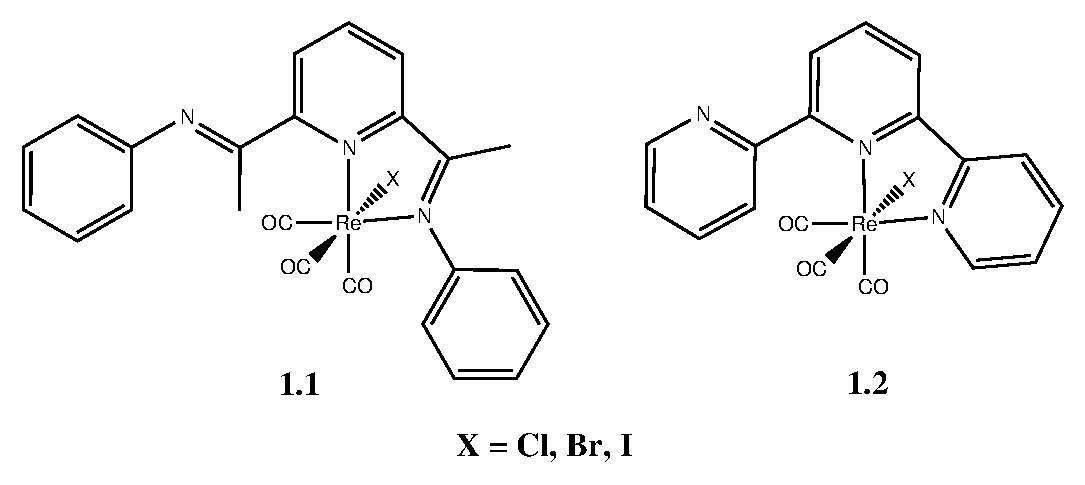
\includegraphics[clip=true, width=110mm]{images/terdentateligands.eps}
 \end{center}
\caption[Two common bidentate complexes using terdentate ligands]{Two common \textit{fac}-\ce{[L2Re(CO)3X]} complexes with terdentate $\sigma$-donor ligands: L = bis(imino)pyridine (\textbf{1.1}) and 2,2':6',2''-terpyridine (\textbf{1.2})}
\label{fig.terdentateligands}
\end{figure}

Further development of this chemistry has been restricted by the limited structural and electronic variability of the common pseudo-octahedral \textit{fac}-\ce{[L2ReX(CO)3]} (\ce{L2} = $\alpha$-diimine) products. While these systems continue to receive considerable attention, studies detailing the coordination chemistry of the meridionally-coordinated tridentate triimine \ce{Re^I} dicarbonyl core are quite limited\autocite{jurca2013}. For example, while \ce{$\kappa$^3(terpy)Re(CO)2Cl} was initially reported in 1988\autocite{juris1988}, closer analysis of the reported analytical data (including \textsuperscript{1}H NMR) indicate that this compound is more likely \ce{$\kappa$^2LRe(CO)3Cl}. A more recent report for this compound provides spectroscopic details of this species as well as the preliminary report for the generation of \ce{[$\kappa$^3(terpy)Re(CO)2L$'$]+} cations (L = \ce{PPh3}, \ce{PEt3}, \ce{NC5H5}, and \ce{NCCH3})\autocite{black2012}. Finally, the \textsuperscript{1}H NMR data for \ce{$\kappa$^3(terpy)Re(CO)2Br} has been reported\autocite{abel1993} but accompanied no other characterization.

In order to fully exploit the potential of this versatile family of compounds, the limits imposed by the bidentate coordination need to be addressed. Furthermore, it would appear that, on the basis of the tridentate ligands that have been investigated, the concerted effort to produce the tridentate species has been essentially unsuccessful, or requiring harsh conditions\autocite{potgieter2013}. Attracted by this challenge we sought to synthesize, crystallographically authenticate, and investigate the photophysical properties of low-valent rhenium pincer complexes displaying an N,N',N''-chelated terpyridine array. 

Complexes of 2,2':6',2''-terpyridine (terpy) are of interest due to the conceptual relationship to established bis(imino)pyridine compounds\autocite{russell2010, tondreau2012}. This thesis will be a discussion of the development of chemistry of \ce{Re^I} complexes, their characterization, and comparison of structural and photo-physical properties to computed values. Further exploration of the \ce{CO2} reduction by photo-catalysis of these new complexes will be analyzed. This thesis will also take a more detailed look at specifics of the mechanisms proposed for current \ce{Re^I} diimine catalysts, and propose new geometries for prior mechanistic steps based on experimental, computational, and literature review work.

%======================================================================
\section{\ce{CO2} Reduction Chemistry}
%======================================================================

Recent years have seen an increase in the concentration of \ce{CO2} in the atmosphere as a product of combustion of oil, gas and coal in the industry and transportation sectors\autocite{song2006}. This is of significant concern due to the greenhouse gas properties of \ce{CO2} \autocite{matthews2009, meinshausen2009}. Attempts to reduce emissions proceed by various pathways, including the utilization of renewable resources such as wind and solar for energy production\autocite{neuhoff2005}; development of more fuel and energy efficient processes; and attempts to capture \ce{CO2} from industrial exhaust streams\autocite{peratitus2014, kadantsev2013, iremonger2011}. It can then be stored in underground depositories, or used as a feedstock in the production of simple molecules or fuels\autocite{leitner1996, olah2009, kang2012}. Due to it being the final product in combustion and its high thermodynamic stability, the reduction of \ce{CO2} is an energy-intensive task\autocite{schwarz1989, morris2009}. While plant life naturally performs \ce{CO2} transformation via photosynthesis, no artificial means have proven to be robust and scalable enough for the task in large scale \autocite{arakawa2001}. 

The development of catalysts for `artificial photosynthesis' has explored various means, including utilizing metal electrodes\autocite{li2010}, electrocatalytic semiconductors (such as \ce{TiO2}, \ce{ZnS}, \ce{CdS}, or As or S doped Ag)\autocite{inoue1971, lim2014}, and organometallic species of Co, Ni, Mn, and Fe (particularly porphyrin complexes)\autocite{fisher1980, tinnemans1984, beley1986, simonmanso2004, fujita1994, fujita1993, kimura1994, dhanasekaran1999, lacy2014, bourrez2011, sampson2014}. These typically require the addition of electrons, and current trends look to solar powered elecricity production for a `green' \ce{CO2} reduction platform\autocite{zeng2014}.

Alternate solutions involves the use of photoredox catalysts, including $\alpha$-diimino complexes of Re\textsuperscript{I}, Ru\textsuperscript{II}, Os\textsuperscript{II}, and Ir\textsuperscript{III}  \autocite{hawecker1983, schneider2011, ishida1987, maidan1986, ishida1990, kitamura1983, tanaka2002, doherty2009, doherty2010, tamaki2013, shunsuke2013, reithmeier2014}. In recent years, the popularity of these $\alpha$-diimino compounds has increased, owing to their unique \gls{ac.mlct} excited states and easily tunable photophysical properties. Of these complexes, Re\textsuperscript{I} based catalysts are of particular interest. Whether acting as a mono-metallic photocatalyst, or with Ru in multi-metallic complexes, the high quantum yield (up to $\Phi$=0.59)\autocite{hori1996, takeda2008} and exclusive selectivity to production of CO is unparalleled in these catalysts\autocite{grills2010, windle2012}. Research focus has turned to tuning photophysical properties for increased use of photons in the visible spectrum (particularly lower energy) and modification of the ligand framework for increased turnover numbers and frequencies \autocite{grills2010, morris2009, shavaleev2004, kutal1985, larsen2014}. This thesis will focus on the synthesis and testing of a novel Re\textsuperscript{I} catalyst attempting to improve on those points.
 %"Organometallic, Photochem & catalysis, rhenium, CO2"
\cleardoublepage
\chapter{New Coordination Geometries for \texorpdfstring{\ce{Re^I}}{Rhenium (I)}}\label{chap.newchem}
\markright{New Coordination Geometries for \texorpdfstring{\ce{Re^I}}{Rhenium (I)}} % new right header
%======================================================================
\section{Introduction}
%======================================================================

As mentioned in the introduction, \ce{Re^I} compounds have been typically bidentate (\ce{$\kappa$^2}) compounds, even when using a potentially terdentate (\ce{$\kappa$^3}) ligand such as bis(imino)pyridine or terpyridine (refer to \autoref{fig.terdentateligands}). The chemistry of this rhenium $\alpha$-diimino complex has been extensively invesigated, with over 1700 references appearing in a SciFinder structure search for that metal-ligand motif\autocite{scifinder}. The ejection of an additional carbonyl and the chelation of the pendant arm of the ligand was attempted to extend the conjugated $\pi$ system of the ligand and its interaction with the metal centre. This was first demonstrated by prior work in our group for the bis(imino)pyridine ligand\autocite{jurca2013}. 

%======================================================================
\section{Synthesis of Bidentate and Terdentate \texorpdfstring{\ce{Re^I}}{Rhenium (I)} Complexes}
%======================================================================

Similar to the prior work, synthesis began with the production of the bidentate complex \ce{$\kappa$^2(terpy)Re(CO)3X} (X = Cl, Br) by coordination of 2,2':6',2''-terpyridine with a \ce{Re(CO)5X} starting material in dry toluene at reflux for 4 hours, as shown in \autoref{scheme.bidentate}. A bright yellow powder precipitated from solution and was collected by filtration, washed with cold hexanes, and dried \textit{in vacuo} to a good yield of \textbf{2.1} and \textbf{2.3} respectively.\footnote{Experimental details for all compounds can be seen in \autoref{app.exp} \nameref{app.exp}} These bidentate compounds were characterized fully and used without further purification to produce \ce{$\kappa$^3(terpy)Re(CO)2X} (X = Cl, Br) via thermolysis, as well as for anion exchange reactions. 

\begin{scheme}[!htb]
 \begin{center}
  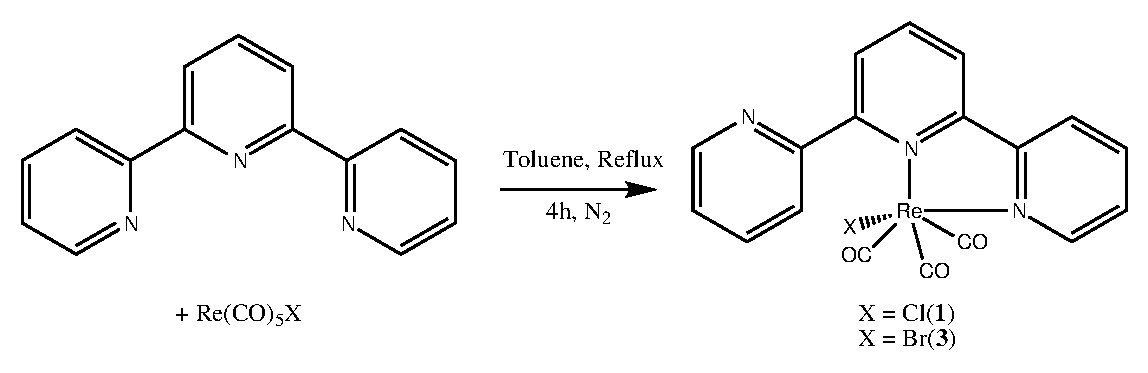
\includegraphics[clip=true, width=140mm, keepaspectratio]{images/bidentate.eps}
 \end{center}
\caption[Synthesis of \textbf{2.1} and \textbf{2.3}]{Synthesis of \textbf{2.1} and \textbf{2.3} from \ce{Re(CO)5X} and 2,2':6',2''-terpyridine}
\label{scheme.bidentate}
\end{scheme} 

Conversion of compounds \textbf{2.1} and \textbf{2.3} to the $\kappa^3$ moiety required the release of \ce{CO} and the subsequent coordination of the free pendant arm. Prior work had identified the thermal lability of the carbonyl, based on a method first described by Buckingham with a osmium complexes\autocite{buckingham1964}. In this method, a ceramic sample boat was placed in a tube furnace at elevated temperature, under a flowing atmosphere of \ce{N2}. After some time, the sample is removed and collected at nearly quantitative yield. Determination of the appropriate thermolysis temperature was performed by \gls{ac.tga} of the sample. A loss of 6-8~\% of starting mass from the sample is consistent with the loss of one carbonyl group from the complex. Results of \gls{ac.tga} on \textbf{2.1} and \textbf{2.3} is shown in \autoref{fig.tga}.

\begin{figure}[!htbp]
 \begin{center}
  \includegraphics[clip=true, width=140mm]{images/tga.eps}
 \end{center}
\caption[Results of \glsentrytext{ac.tga} analysis on \textbf{2.1} and \textbf{2.3}]{Results of \glsentrytext{ac.tga} analysis on \textbf{2.1} (blue) and \textbf{2.3} (green).}
\label{fig.tga}
\end{figure} 

The onset of mass loss in the \gls{ac.tga} of \textbf{2.1}, and the onset of the main mass loss in the \gls{ac.tga} of \textbf{2.3} were chosen to identify a thermolysis temperature for each sample. For \textbf{2.1}, thermolysis was performed at 240~$^\circ$C, and for \textbf{2.3} thermolysis was performed at 260~$^\circ$C, yielding \textbf{2.2} and \textbf{2.4} respectively, at quantitative yields, by the pathway in \autoref{scheme.terdentate}.

\begin{scheme}[!htb]
 \begin{center}
  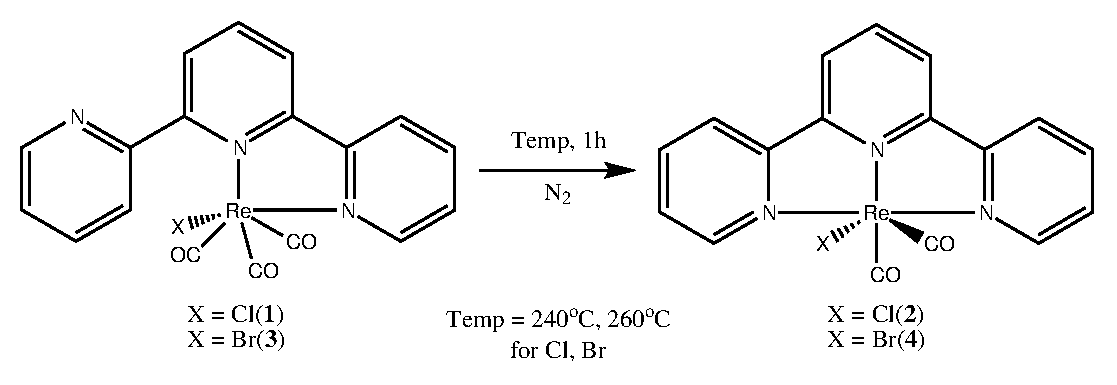
\includegraphics[clip=true, width=140mm, keepaspectratio]{images/thermolysis.eps}
 \end{center}
\caption[Synthesis of \textbf{2.2} and \textbf{2.4}]{Synthesis of \textbf{2.2} and \textbf{2.4} by thermolysis of \textbf{2.1} or \textbf{2.3}, respectively}
\label{scheme.terdentate}
\end{scheme} 

\begin{scheme}[!htbp]
 \begin{center}
  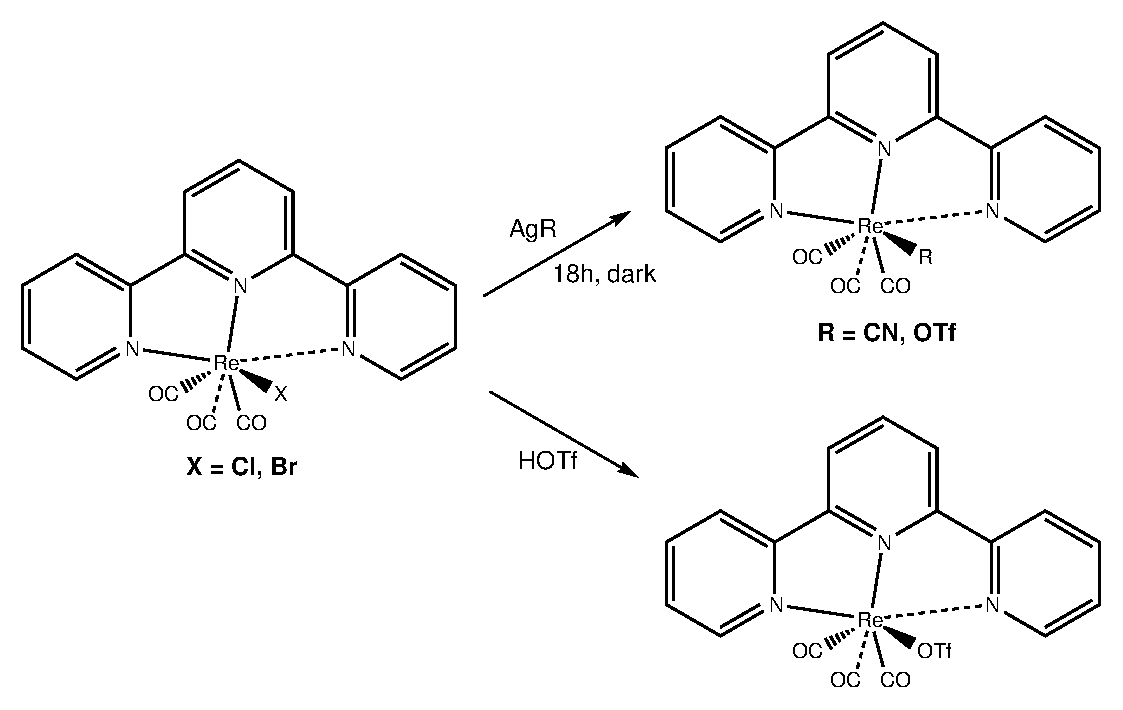
\includegraphics[clip=true, keepaspectratio, width=120mm]{images/anionscheme.eps}
 \end{center}
\caption[Anion exchange pathways]{Anion exchange pathways to synthesize \textbf{2.5} - \textbf{2.8}}
\label{scheme.anion}
\end{scheme}

Further reactions were carried out on the above products to yield triflate and cyano complexes in bidentate and terdentate geometries. These anion exchange reactions were performed by the addition of the silver salt to the chloride products \textbf{2.1} or \textbf{2.2}, to precipitate \ce{AgCl}, leaving \ce{$\kappa$^2(terpy)Re(CO)3CN} (\textbf{2.5}), \ce{$\kappa$^3(terpy)Re(CO)2CN} (\textbf{2.6}), \ce{$\kappa$^2(terpy)Re(CO)3OTf} (\textbf{2.7a}) and \ce{$\kappa$^3(terpy)Re(CO)2OTf} (\textbf{2.8a}), as shown in \autoref{scheme.anion}. Reaction with the bromide products proceeds with similar results. As the Ag anion exchange reactions result in only moderate yields, \textbf{2.7b} was synthesized by the direct addition of neat triflic acid (\ce{CF3SO3H}) to \textbf{2.1}. \ce{HCl} was released, the solutions were quenched by addition of dilute aqueous \ce{NaCO3}, and product was collected via separation into chloroform, again at moderate yield. 

%======================================================================
\section{Characterization}
%======================================================================

Full characterization was performed, including \Gls{ac.nmr} analysis, x-ray crystallography, elemental analysis, as well as UV-Vis and IR spectroscopy. Computational \gls{ac.dft} methods were used to solve the geometries, and \gls{ac.tddft} was performed to predict UV-Vis spectra and identify electronic transitions. 

%----------------------------------------------------------------------
\subsection{NMR Analysis}
%----------------------------------------------------------------------

Proton \gls{ac.nmr} was performed on each of the samples. Each sample was dissolved completely in deuterated acetonitrile (\ce{CD3CN}) and analysis was performed on a Bruker AVANCE 400 MHz spectrometer. Data was processed from the FID signal via the TopSpin program, and spectra were analyzed using ACD~nmR Processor v12.0. 

Detailed peak analysis comparing bidentate samples \textbf{2.1}, \textbf{2.3}, \textbf{2.5}, and \textbf{2.7} (\autoref{fig.bid4nmr}) or terdentate \textbf{2.2}, \textbf{2.4}, \textbf{2.6}, and \textbf{2.8} (\autoref{fig.ter4nmr}) show little difference between samples. This is due to the distance between the anion and any protons on the ligand. Anions with different $\sigma$-donor strength marginally impact the metal-ligand interactions; these have only small effect on the location of peaks, shifting between samples by typically less than 0.1~ppm. As is shown in \autoref{fig.bid4nmr}, the characteristic shape of each spectra remains constant, only exact peak locations and some peak order varies with anion choice. 


\begin{figure}[!htb]
 \begin{center}
  \includegraphics[clip=true, width=\textwidth, keepaspectratio]{images/allbidnmr.eps}
 \end{center}
\caption[The aromatic region of the \texorpdfstring{\ce{^1H}}{1H} \glsentrytext{ac.nmr} spectra of the four bidentate compounds]{The aromatic region of the \texorpdfstring{\ce{^1H}}{1H} \glsentrytext{ac.nmr} spectra for compounds \textbf{2.1} (blue), \textbf{2.3} (green), \textbf{2.5} (red) and \textbf{2.7} (purple)}
\label{fig.bid4nmr}
\end{figure} 

The characteristic feature in the \gls{ac.nmr} spectra after the transformation from bidentate to terdentate (e.g. sample \textbf{2.1} to \textbf{2.2}) is the reduction in the total number of the signals in the aromatic region (between 7 and 9~ppm). This simplification is due to the increased symmetrization of the ligand, while the \ce{$\kappa$^2}-bidentate ligand has a freely rotating pendant group. Prior work in literature\autocite{abel1993} and in our group\autocite{jurca2012} shows the temperature dependence of the rate of rotation of this pendant arm for various ligand species. However, the \ce{$\kappa$^3}-terdentate species has no free groups, the rigid geometry and higher order symmetry results in the simpler \gls{ac.nmr} spectrum.

\begin{figure}[!htb]
 \begin{center}
  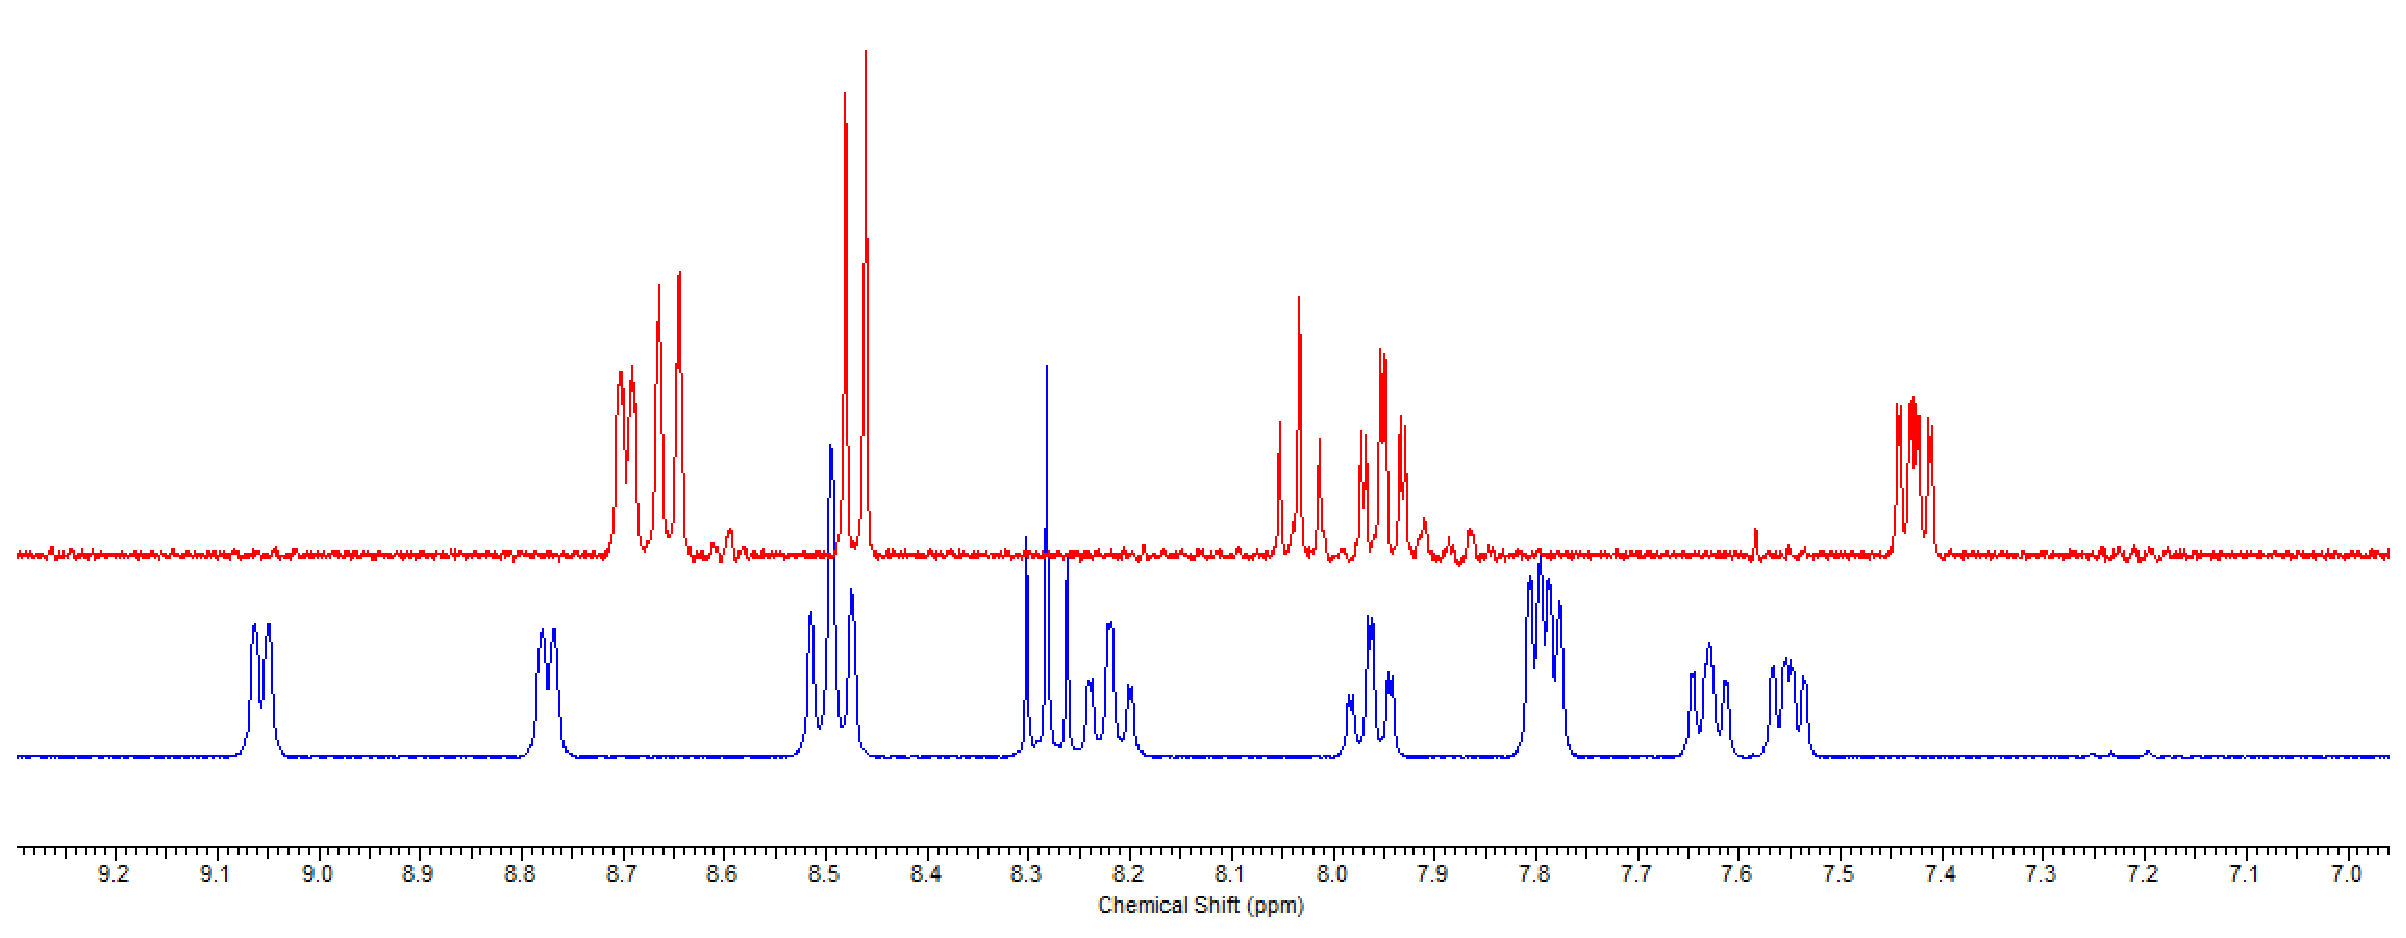
\includegraphics[clip=true, width=\textwidth, keepaspectratio]{images/bidternmr.eps}
 \end{center}
\caption[The aromatic region of the \texorpdfstring{\ce{^1H}}{1H} \glsentrytext{ac.nmr} spectra showing bidentate - terdentate conversion]{The aromatic region of the \texorpdfstring{\ce{^1H}}{1H} \glsentrytext{ac.nmr} spectra for compounds \textbf{2.1} (blue) and \textbf{2.2} (red), showing the simplification of the spectra upon the conversion from bidentate to terdentate}
\label{fig.bidtoter}
\end{figure} 

\begin{figure}[!htb]
 \begin{center}
  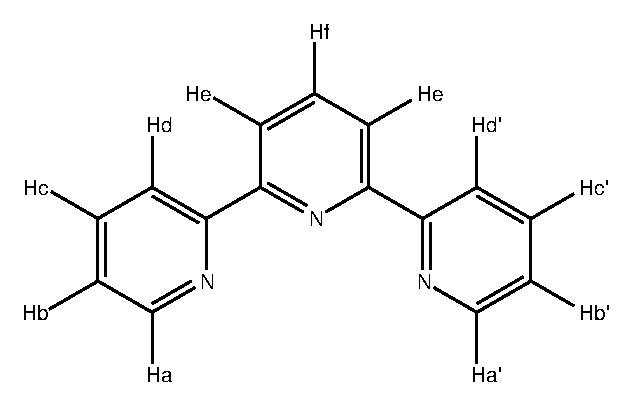
\includegraphics[clip=true, width=80mm, keepaspectratio]{images/expandedterpyridine.eps}
 \end{center}
\caption[Proton-explicit skeletal drawing of 2,2':6',2''-terpyridine]{Proton-explicit skeletal drawing of 2,2':6',2''-terpyridine}
\label{fig.terpynmr}
\end{figure} 

The simplification of peaks due to the symmetrization of the ligand results in the peaks from free pendant arm protons \textit{a}, \textit{b}, \textit{c}, and \textit{d} (see \autoref{fig.terpynmr}) with peaks at 9.06, 7.63, 8.22 and 7.79~ppm, respectively, aligning with their mirroring peaks at \textit{a'}, \textit{b'}, \textit{c'} and \textit{d'} (with peaks at 8.77, 7.55, 7.96, and 7.80~ppm). The new symmetrized peaks show integrations of two protons per peak, relative to the single proton (\textit{f}) peak from the central pyridyl ring, \textit{para} to the nitrogen. As well, the presence of metal-ligand interaction in the pendant arms reduces the deshielding effect, shifting the free pyridyl \textit{ortho} proton from 9.06 to 8.77~ppm in the chelated group, with similar shifts evident for the other pendant protons.

As in the case of bidentate compounds, modification of the anion has only minor effects on the \gls{ac.nmr} spectra. This is the expected behaviour, the conjugated pi system and the lack of protons near the modified anion combine to be susceptible in only a minor fashion.  

\begin{figure}[!htb]
 \begin{center}
  \includegraphics[clip=true, width=\textwidth, keepaspectratio]{images/allternmr.eps}
 \end{center}
\caption[The aromatic region of the \texorpdfstring{\ce{^1H}}{1H} \glsentrytext{ac.nmr} spectra of the four terdentate compounds]{The aromatic region of the \texorpdfstring{\ce{^1H}}{1H} \glsentrytext{ac.nmr} spectra for compounds \textbf{2.2} (blue), \textbf{2.4} (green), \textbf{2.6} (red) and \textbf{2.8} (purple)}
\label{fig.ter4nmr}
\end{figure} 

Carbon \gls{ac.nmr} (\ce{^{13}C}) was attempted on the complexes as well. Unfortunately, \ce{Re^I} complexes perform poorly in \ce{^{13}C}~\gls{ac.nmr} experiments, the signal to noise ratio is incredibly poor (if a signal is even visible). The effect of this is a lack of \ce{^{13}C} \gls{ac.nmr} analysis of these compounds in literature, with very few exceptions\autocite{morimoto2013}. Extensive efforts included use of a 500 MHz spectrometer, with 1664 scans to produce the best example, seen in \autoref{fig.13cnmr}, with average peak signal to noise ratio (s/n) of only 4~-~5.

\begin{figure}[!htb]
 \begin{center}
  \includegraphics[clip=true, width=\textwidth, keepaspectratio]{images/13cnmr.eps}
 \end{center}
\caption[The 13C \glsentrytext{ac.nmr} spectra of \textbf{2.1}]{The \ce{^{13}C} \glsentrytext{ac.nmr} spectra of \textbf{2.1}. Spectra for other compounds could not be collected}
\label{fig.13cnmr}
\end{figure} 

\FloatBarrier

%----------------------------------------------------------------------
\subsection{Structure Analysis with X-Ray Crystallography and DFT}\label{ss.xray}
%----------------------------------------------------------------------

Single crystal analysis by x-ray crystallography yielded good structures of compounds \textbf{2.1}, \textbf{2.2}, \textbf{2.3}, \textbf{2.5}, and \textbf{2.8}. These are the first reported crystal structures of the $\kappa^3$~terdentate \ce{Re^I} compounds. A number of structural characteristics are common between the various bidentate or terdentate complexes. Much analysis has been done on the structures of bidentate complexes in literature\autocite{anderson1990, civitello1993, kurz2006} the notable characteristic within terpyridine compounds is the rotation of the pendant arm, pushing the nitrogen atom away from the plane of the metal-ligand bonds by approximately 100$^\circ$. Cell parameters and other collection data for compounds \textbf{2.1}, \textbf{2.3}, \textbf{2.5}, and \textbf{2.7} are located in \autoref{tab.bidxraycp}.

% Table generated by Excel2LaTeX

\begin{table}[!htb]
  \caption{Crystal data and structure refinement for compounds \textbf{2.1}, \textbf{2.3}, and \textbf{2.5}}
  \resizebox{\textwidth}{!}{%
  \begin{tabular}{rp{3.2cm}p{3.2cm}p{3.2cm}}
    \toprule
    Compound & \textbf{2.1} & \textbf{2.3} & \textbf{2.5}  \\
    \cmidrule(l){2-4} 
    Empirical formula & \ce{C19H11N3O3ReCl} & \ce{C19H11N3O3ReBr} & \ce{C20H11N4O3Re} \\
    Formula weight (g/mol) & 538.96 & 583.41 & 530.04 \\
    Temperature (K) & 200 & 200 & 200 \\
    Wavelength (\r{A})  & 0.71073 & 0.71073 & 0.71073 \\
    Crystal System & Triclinic & Monoclinic & Triclinic \\
    Space Group & P-1 & C2/c & P-1  \\
    a (\r{A}) & 9.8736(4) & 31.1537(7) & 9.9196(9) \\
    b (\r{A}) & 14.8202(4) & 7.1176(2) & 14.9902(14) \\
    c (\r{A}) & 16.3472(4) & 16.8519(4) & 16.5187(15) \\
    $\alpha$ (deg) & 69.2890(10) & 90.000 & 68.363(2) \\
    $\beta$ (deg) & 80.801(2) & 111.0230(10) & 80.929(2) \\
    $\gamma$ (deg) & 79.836(2) & 90.000 & 79.975(2) \\
    Volume (\r{A}\textsuperscript{3}) & 2190.00(12) & 3488.00 & 2236.6(4) \\
    Z, r (calc) (Mg/m\textsuperscript{3}) & 2, 1.997 & 8, 2.222 & 2, 1.927 \\
    Absorption coefficient (mm\textsuperscript{-1}) & 6.063 & 9.282 & 5.821 \\
    Absorption correction  & \multicolumn{3}{c}{Semi-empirical from equivalents} \\
    Final R indices [I$\geq$2$\sigma$(I)] & R1 = 0.0397,\newline wR2 = 0.0839 & R1 = 0.0232,\newline wR2 = 0.0614 & R1 = 0.0390,\newline wR2 = 0.0921 \\
    R indices (all data) & R1 = 0.0604,\newline wR2 = 0.0951 & R1 = 0.0285,\newline wR2 = 0.0642 & R1 = 0.0500,\newline wR2 = 0.0961 \\
    \bottomrule
  \end{tabular}} 
  \label{tab.bidxraycp}%
\end{table}%



In addition, the structures of all species were optimized using Gaussian 09\autocite{gaussian} employing the B3LYP\autocite{becke1993, lee1988}  exchange-correlation (XC) functional. The LanL2DZ basis set/effective core potential was used on Re\autocite{hay1985}, and the all-electron TZVP basis set for the remaining lighter atoms\autocite{schafer1994}. Frequency analysis of all structures was used to confirm the nature of the stationary points. Solvent effects were computed when necessary using the integral equation formalism variant of the \gls{ac.pcm} for solvation within Gaussian 09\autocite{tomasi2005, scalmani2006}.The results of these calculations are compared to the x-ray crystallography data in the tables below.

The crystal structure of \textbf{2.3} had a higher symmetry than the other samples. Details on the exact methods used for structure elucidation are available in \autoref{sec.xray}, but all of the structures found are of high quality. The structures of \textbf{2.1}, \textbf{2.3}, and \textbf{2.5} can be seen in \autoref{fig.xraybid}. More views of these structures can be seen in Appendix \autoref{sec.xray}. Crystals suitable for x-ray analysis were unable to be collected from compound \textbf{2.7}. 

\begin{figure}[!ht]
 \centering
 \begin{subfigure}[b]{0.49\textwidth}
  \includegraphics[clip=true, width=\textwidth, keepaspectratio]{images/xray1a.eps}
  \caption{X-ray crystal structure for \textbf{2.1}}
  \label{fig.da1}
 \end{subfigure}
 \begin{subfigure}[b]{0.49\textwidth}
  \includegraphics[clip=true, width=\textwidth, keepaspectratio]{images/xray3a.eps}
  \caption{X-ray crystal structure for \textbf{2.3}}
  \label{fig.da3}
 \end{subfigure}
 \begin{subfigure}[b]{0.49\textwidth}
  \includegraphics[clip=true, width=\textwidth, keepaspectratio]{images/xray5a.eps}
  \caption{X-ray crystal structure for \textbf{2.5}}
  \label{fig.da5}
 \end{subfigure}
\caption[X-ray crystal structure representation for \textbf{2.1}, \textbf{2.3} and \textbf{2.5}.]{X-ray crystal structure representation for \textbf{2.1}, \textbf{2.3}, and \textbf{2.5}. Co-crystallized chloroform, hydrogen atoms, and thermal ellipsoids of ligand carbon atoms are omitted for clarity.}
\label{fig.xraybid}
\end{figure}

Selected bond lengths, bond angles, and torsion angles are listed in \autoref{tab.da1}, \autoref{tab.da3} and \autoref{tab.da5} for products \textbf{2.1}, \textbf{2.3}, and \textbf{2.5} respectively. The experimental results agree closely with the computed values for all samples. The structures can be seen in \autoref{fig.da1}, \autoref{fig.da3} and \autoref{fig.da5}, and more views of these structures can be seen in \autoref{app.xrays}, \nameref{app.xrays}. 

The \ce{Re^I} centre in the pseudooctahedral complex is supported by a planar, pincer coordinated ligand defined by the terminal and central pyridyl group of the terpyridine. One of the carbonyl groups lies in this plane trans to the central pyridyl group, while the remaining carbonyl groups and the anionic group or other complexed species lie on an approximately perpendicular plane to the ligand. Bond angles around the Re centre show a significant deviation of up to 15$^\circ$ from the ideal octahedral geometry for all samples analyzed. The typical N-Re-N bond angle of 75$^\circ$ is due to the atomic size of rhenium, comparison to the crystal structure of an analogous compound with a manganese atom\autocite{compain2014} shows a decrease in the bonding angle for the \ce{Re} complex by approximately 4$^\circ$ due to an increase of bond length from metal to nitrogen of about 0.12~\r{A} for both the central and terminal pyridines. 

The deviation from octahedral is further visible in the rotation of the X-Re-CO plane (X=halide, anion, or other complexed group) by approximately 10 degrees from the right angle relative to the plane of the ligand. The axial halide, anion, or chelated group typically occupies a position slightly departed from the perpendicular, angled to be over the ligand. This eclipsing is due to some unknown process, no steric interference exists upon that site, analysis of electrostatic or other short-range electronic effects computationally show any interaction between this site and the aromatic rings. In \ce{Re^I} complexes, the halide or anion is located axial relative to the plane of the ligand. For the acetonitrile complex with triflate counterion, the acetonitrile occupies the axial position. This site occupation holds through the complete set of x-ray crystal structures with a \ce{$\kappa$^2-(bipy)Re(CO)3X} core structure motif deposited in the \gls{ac.ccdc} database\autocite{allen2002}, and extends through other $\alpha$-diimine complexes seen in our lab and in literature\autocite{jurca2013}. 

% Table generated by Excel2LaTeX
\begin{table}[!h]
\centering
 \begin{threeparttable}
  \caption{Solvated and gas phase energy differences between Axial \& Trans geometries of \ce{$\kappa$^x-(terpy)-Re(CO)_{5-x}CN} (x=2,3)}
    \begin{tabular}{cccc}
    \toprule
    \multicolumn{2}{c}{Bidentate} & \multicolumn{2}{c}{Terdentate} \\ \midrule
    E(gas)\tnote{a} & E(solution)\tnote{b} & E(gas)\tnote{a} & E(solution)\tnote{b} \\ \midrule
    14.70 & 11.87 & 16.28 & 16.43 \\
    \bottomrule
    \end{tabular}%
    \begin{tablenotes}
    \item [a] B3LYP SCF energy in kcal/mol.
    \item [b] B3LYP SCF energy in kcal/mol, with PCM solvation in acetonitrile.
    \end{tablenotes}
  \label{tab.cneng}%
 \end{threeparttable}
\end{table}%




The crystal structure for compound \textbf{2.5} contains two molecules per unit cell, one of which is solved to have the cyano group in the position trans to the ligand. However, careful analysis of the bond lengths, angles, and torsion data in \autoref{tab.da5} shows a remarked similarity between all -CO and -CN groups. Additionally, in an x-ray diffraction pattern, -CN and -CO are difficult to differentiate with certainty. Thus, while the structure solved to the two isomers, critical analysis would suggest that this molecule does not violate the axial position pattern laid out above. The computed structures energies in \autoref{tab.cneng} show a favouring of the axial position by 12-16 kJ/mol in the gas phase and by \gls{ac.pcm} in a simulated acetonitrile solvent. 

Selected bond lengths, bond angles, and torsions are listed in \autoref{tab.da1}, \autoref{tab.da3} and \autoref{tab.da5} for products \textbf{2.1}, \textbf{2.3}, and \textbf{2.5} respectively.

% Table generated by Excel2LaTeX
\begin{table}[htbp]
  \caption{Selected Distances, Angles, and Torsions for \textbf{1}}
  \centering
    \begin{tabular}{ccc}
    \toprule
    \multirow{2}{*}{Bond} & \multicolumn{2}{c}{Distance (\r{A})} \\ \cline{2-3}
     & Experimental & Calculated \\ \midrule
    Re(1)-C(16) & 1.89(1) & 1.916 \\
    Re(1)-C(17) & 1.934(8) & 1.936 \\
    Re(1)-C(18) & 1.90(1) & 1.918 \\
    Re(1)-N(1) & 2.162(6) & 2.197 \\
    Re(1)-N(2) & 2.236(9) & 2.293 \\
    Re(1)-Cl(1) & 2.496(2) & 2.525 \\ \midrule
    \multirow{2}{*}{Angle} & \multicolumn{2}{c}{Degrees ($^\circ$)} \\ \cline{2-3}
     & Experimental & Calculated \\ \midrule
    C(16)-Re(1)-C(17) & 87.6(4) & 86.877 \\
    C(16)-Re(1)-C(18) & 88.3(4) & 90.613 \\
    C(17)-Re(1)-C(18) & 87.3(4) & 89.557 \\
    C(16)-Re(1)-N(1) & 96.4(3) & 96.240 \\
    C(17)-Re(1)-N(1) & 174.9(3) & 175.600 \\
    C(18)-Re(1)-N(1) & 95.9(3) & 93.506 \\
    C(16)-Re(1)-N(2) & 169.3(3) & 170.368 \\
    C(17)-Re(1)-N(2) & 101.1(3) & 102.755 \\
    C(18)-Re(1)-N(2) & 98.3(3) & 89.415 \\
    N(2)-Re(1)-N(1) & 74.5(3) & 74.146 \\
    C(16)-Re(1)-Cl(1) & 91.7(3) & 91.453 \\
    C(17)-Re(1)-Cl(1) & 91.7(3) & 94.786 \\
    C(18)-Re(1)-Cl(1) & 179.9(3) & 175.286 \\
    N(1)-Re(1)-Cl(1) & 84.0(2) & 82.058 \\
    N(2)-Re(1)-Cl(1) & 81.6(2) & 87.840 \\
    O(1)-C(16)-Re(1) & 179.6(9) & 178.224 \\
    O(2)-C(17)-Re(1) & 176.0(8) & 176.907 \\ 
    O(3)-C(18)-Re(1) & 177.3(9) & 179.317 \\ \midrule
    \multirow{2}{*}{Torsion} & \multicolumn{2}{c}{Degrees ($^\circ$)} \\ \cline{2-3}
     & Experimental & Calculated \\ \midrule
    N(1)-C(5)-C(6)-N(2) &  16(1) & 15\\
    N(2)-C(10)-C(11)-N(3) & 41(1) & 139\\
    \bottomrule
    \end{tabular}%
  \label{tab.da1}%
\end{table}%



% Table generated by Excel2LaTeX
\begin{table}[htbp]
  \caption{Selected Distances, Angles, and Torsions for \textbf{2.3}}
  \centering
    \begin{tabular}{ccc}
    \toprule
   \multirow{2}{*}{Bond} & \multicolumn{2}{c}{Distance (\r{A})} \\ \cline{2-3}
     & Experimental & Calculated \\ \midrule
    Re(1)-C(16) & 1.911(3) & 1.91740 \\
    Re(1)-C(17) & 1.890(3) & 1.91814 \\
    Re(1)-C(18) & 1.921(4) & 1.93897 \\
    Re(1)-N(1) & 2.173(3) & 2.19687 \\
    Re(1)-N(2) & 2.232(2) & 2.28998 \\
    Re(1)-Br(1) & 2.6410(4) & 2.67953 \\ 
    C(16)-O(1) & 1.150(4) & 1.15290 \\
    C(17)-O(2) & 1.157(4) & 1.15012 \\
    C(18)-O(3) & 1.155(5) & 1.15591 \\ \midrule
    \multirow{2}{*}{Angle} & \multicolumn{2}{c}{Degrees ($^\circ$)} \\ \cline{2-3}
     & Experimental & Calculated \\ \midrule
    C(16)-Re(1)-C(17) & 89.1(1) & 90.772 \\
    C(16)-Re(1)-C(18) & 85.9(1) & 86.823 \\
    C(16)-Re(1)-N(1) & 97.9(1) & 96.034 \\
    C(17)-Re(1)-N(1) & 92.5(1) & 93.597 \\
    C(18)-Re(1)-N(1) & 175.4(1) & 175.575 \\
    C(16)-Re(1)-N(2) & 171.2(1) & 170.290 \\
    C(17)-Re(1)-N(2) & 96.0(1) & 89.435 \\
    C(18)-Re(1)-N(2) & 101.3(1) & 102.886 \\
    N(1)-Re(1)-N(2) & 74.7(1) & 74.265 \\
    C(16)-Re(1)-Br(1) & 92.7(1) & 90.399 \\
    C(17)-Re(1)-Br(1) & 177.6(1) & 176.076 \\
    C(18)-Re(1)-Br(1) & 91.6(1) & 94.069 \\
    N(1)-Re(1)-Br(1) & 85.74(7) & 82.555 \\
    N(2)-Re(1)-Br(1) & 82.07(7) & 88.780 \\
    O(1)-C(16)-Re(1) & 178.6(3) & 178.270 \\
    O(2)-C(17)-Re(1) & 179.5(3) & 179.355 \\
    O(3)-C(18)-Re(1) & 179.9(3) & 176.781 \\\midrule
    \multirow{2}{*}{Torsion} & \multicolumn{2}{c}{Degrees ($^\circ$)} \\ \cline{2-3}
     & Experimental & Calculated \\ \midrule
    N(1)-C(6)-C(1)-N(2) & -15.4(4) & -14.749 \\
    N(2)-C(5)-C(11)-N(3) & 141.1(3) & 136.119 \\
    \bottomrule
    \end{tabular}%
  \label{tab.da3}%
\end{table}%



% Table generated by Excel2LaTeX
\begin{table}[htbp]
  \caption{Selected Distances, Angles, and Torsions for \textbf{5}}
  \centering
    \begin{tabular}{cccc}
    \toprule
    \multicolumn{4}{c}{Selected Distances (\r{A})} \\ \midrule
    \multicolumn{2}{c}{Cyanide Axial} & \multicolumn{2}{c}{Cyanide Trans} \\ \midrule
    Re(2)-C(35) & 2.148(7) & Re(1)-C(19) & 2.105(8) \\
    Re(2)-C(36) & 1.926(6) & Re(1)-C(16) & 1.928(5) \\
    Re(2)-C(37) & 1.954(7) & Re(1)-C(18) & 1.96(1) \\
    Re(2)-C(38) & 1.902(9) & Re(1)-C(17) & 1.918(7) \\
    Re(2)-N(5) & 2.242(7) & Re(1)-N(1) & 2.253(5) \\
    Re(2)-N(6) & 2.168(5) & Re(1)-N(2) & 2.176(4) \\
    C(35)-N(8) & 1.138(9) & C(19)-O(3) & 1.17(1) \\
    C(36)-O(4) & 1.145(8) & C(16)-N(4) & 1.149(7) \\
    C(37)-O(5) & 1.151(9) & C(18)-O(2) & 1.14(1) \\
    C(38)-O(6) & 1.17(1) & C(17)-O(1) & 1.130(8) \\ \midrule
    \multicolumn{4}{c}{Selected Angles (deg)} \\ \midrule
    \multicolumn{2}{c}{Cyanide Axial} & \multicolumn{2}{c}{Cyanide Trans} \\ \midrule
    C(16)-Re(1)-C(17) & 87.8(3) & C(36)-Re(2)-C(38) & 87.7(3) \\
    C(16)-Re(1)-C(18) & 87.0(3) & C(36)-Re(2)-C(37) & 88.0(3) \\
    C(16)-Re(1)-C(19) & 92.5(3) & C(36)-Re(2)-C(35) & 92.1(3) \\
    C(17)-Re(1)-C(18) & 88.7(3) & C(38)-Re(2)-C(37) & 88.5(3)\\
    C(17)-Re(1)-C(19) & 90.5(3) & C(38)-Re(2)-C(35) & 90.8(3)\\
    C(18)-Re(1)-C(19) & 179.1(3) & C(37)-Re(2)-C(35) & 179.2(3) \\
    C(16)-Re(1)-N(1) & 102.2(2) & C(36)-Re(2)-N(5) & 100.6(3) \\
    C(16)-Re(1)-N(2) & 175.9(2) & C(36)-Re(2)-N(6) & 174.2(3) \\
    C(17)-Re(1)-N(1) & 168.3(3) & C(38)-Re(2)-N(5) & 169.3(3) \\
    C(17)-Re(1)-N(2) & 95.9(3) & C(38)-Re(2)-N(6) & 96.6(3) \\
    C(18)-Re(1)-N(1) & 97.7(3) & C(37)-Re(2)-N(5) & 98.4(2) \\
    C(18)-Re(1)-N(2) & 94.8(3) & C(37)-Re(2)-N(6) & 96.0(2) \\
    C(19)-Re(1)-N(1) & 83.2(2) & C(35)-Re(2)-N(5) & 82.3(2) \\
    C(19)-Re(1)-N(2) & 85.7(2) & C(35)-Re(2)-N(6) & 83.9(2) \\
    N(1)-Re(1)-N(2) & 73.9(2) & N(5)-Re(2)-N(6) & 74.7(2) \\
    O(1)-C(17)-Re(1) & 178.2(7) & O(6)-C(38)-Re(2) & 179.4(7) \\
    O(2)-C(18)-Re(1) & 172.0(7)& O(5)-C(37)-Re(2) & 175.5(6) \\ 
    O(3)-C(19)-Re(1) & 178.0(6) & N(8)-C(35)-Re(2) & 178.0(6) \\
    N(4)-C(16)-Re(1) & 178.7(6) & O(4)-C(36)-Re(2) & 179.0(7) \\ \midrule
    \multicolumn{4}{c}{Selected Torsions (deg)} \\ \midrule
    \multicolumn{2}{c}{Cyanide Axial} & \multicolumn{2}{c}{Cyanide Trans} \\ \midrule
    N(1)-C(1)-C(6)-N(2) & 12.5(8) & N(5)-C(20)-C(25)-N(6) & 14.5(9) \\
    N(1)-C(5)-C(11)-N(3) & 43.7(9) & N(5)-C(24)-C(30)-N(7) & 41(1) \\
    \bottomrule
    \end{tabular}%
  \label{tab.da5}%
\end{table}%




\FloatBarrier

Structural comparisons between the bidentate samples and the terdentate show many similarities. The loss of one carbonyl always accompanies the chelation of the pendant arm of the ligand. The increased coordination forces the ligand to adopt a more rigidly planar geometry, this is visible in the structure of \textbf{2.2} (\autoref{fig.da2}) and \textbf{2.8} (\autoref{fig.da8}). Suitable crystals for x-ray analysis were unable to be collected for the remaining complexes.

\begin{figure}[!ht]
 \centering
 \begin{subfigure}[b]{0.49\textwidth}
  \includegraphics[clip=true, width=\textwidth, keepaspectratio]{images/xray2a.eps}
  \caption{X-ray crystal structure for \textbf{2.2}}
  \label{fig.da2}
 \end{subfigure}
 \begin{subfigure}[b]{0.49\textwidth}
  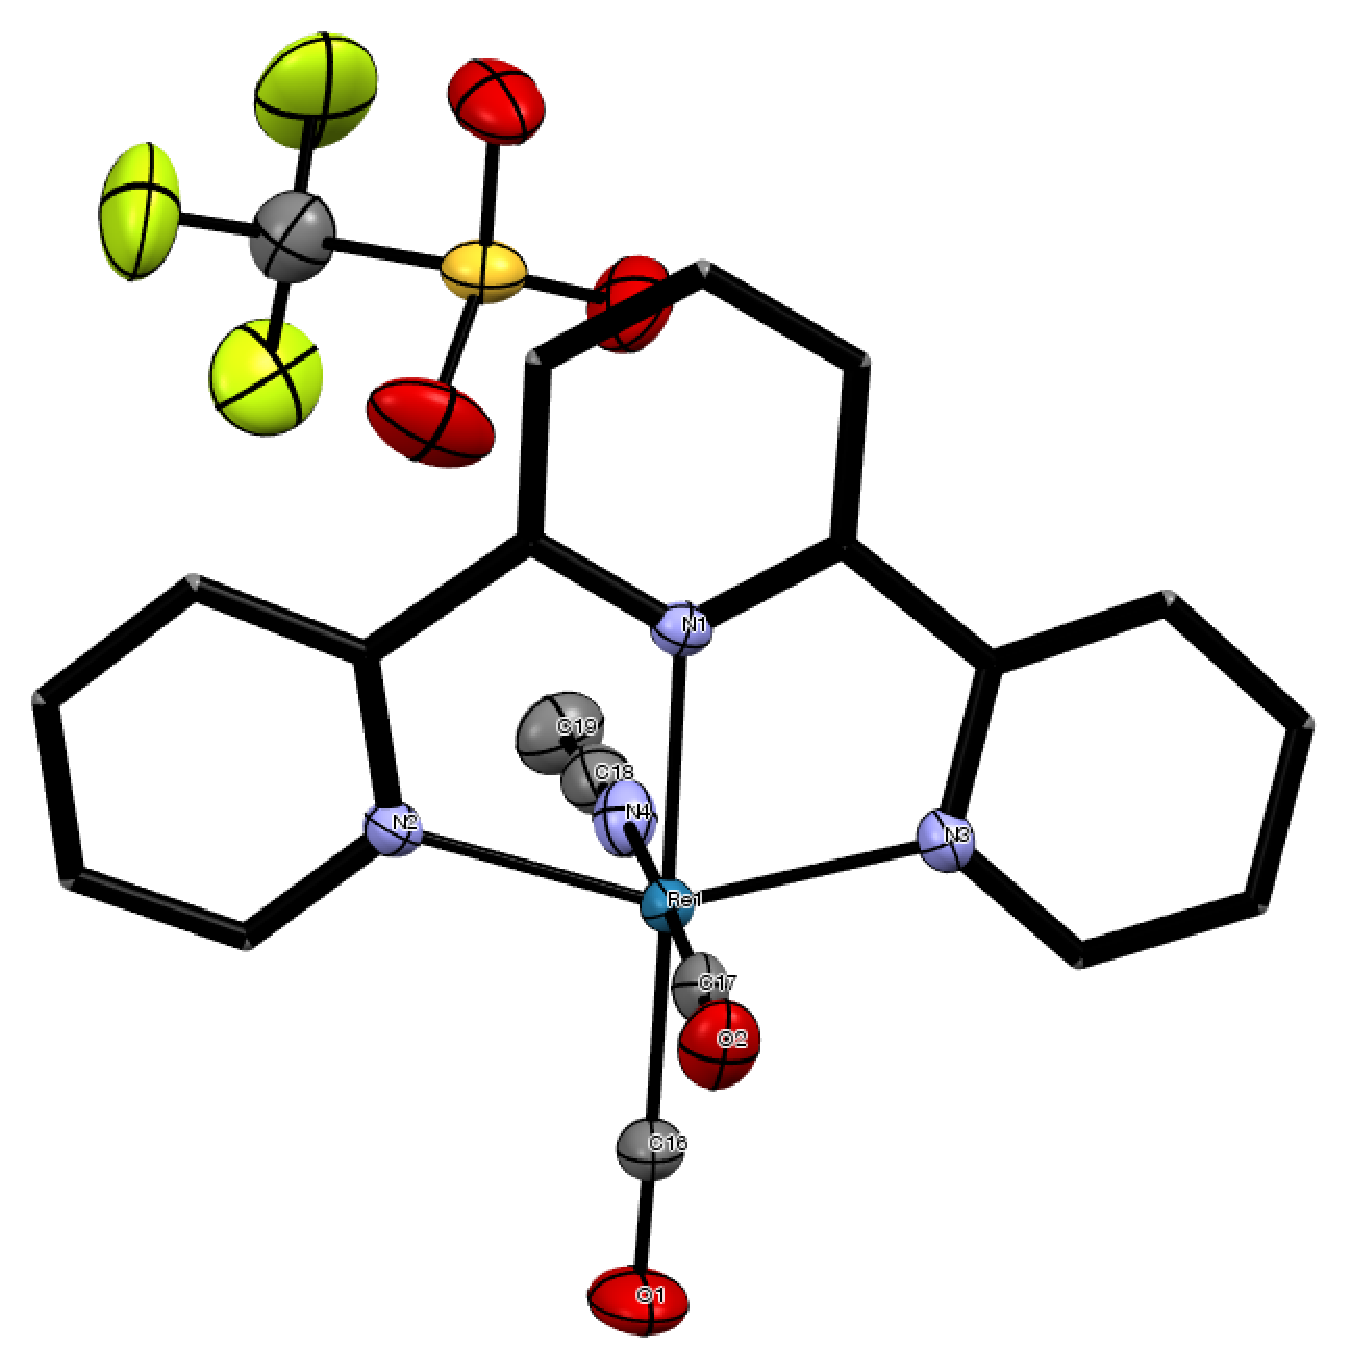
\includegraphics[clip=true, width=\textwidth, keepaspectratio]{images/xray8a.eps}
  \caption{X-ray crystal structure for \textbf{2.8}}
  \label{fig.da8}
 \end{subfigure}
\caption[X-ray crystal structure representation for \textbf{2} and \textbf{8}.]{X-ray crystal structure representation for \textbf{2.2} and \textbf{2.8}. Co-crystallized chloroform, hydrogen atoms, and thermal ellipsoids of ligand carbon atoms are omitted for clarity.}
\label{fig.xrayter}
\end{figure} 

Selected bond lengths, bond angles, and torsions are listed in \autoref{tab.da2} and \autoref{tab.da8} for products \textbf{2.2} and \textbf{2.8}. Cell parameters and collection data can be found in \autoref{tab.tercellparams}. 

Both \textbf{2.2} and \textbf{2.8} structures are pseudooctahedral in geometry, with \textit{mer} coordinated terpyridine ligand. The carbonyl groups and chloride/acetonitrile form a plane approximately perpendicular to the ligand. As in the \ce{$\kappa$^2}-bidentate samples discussed above, the carbonyls occupy the equatorial and one axial position relative to the ligand, and the chloride or acetonitrile occupy the remaining axial position. The N-Re-N bond angles remain approximately 75$^\circ$, and the central pyridyl N to chloride or acetonitrile angle is still approximately 80-85$^\circ$. 

Comparisons between the \ce{$\kappa$^2}-bidentate and \ce{$\kappa$^3}-terdentate samples (\textbf{2.1} and \textbf{2.2}) highlight the geometrical changes experienced in the thermolysis reaction. The distance from Re to the central pyridyl N has shortened from 2.24~to~2.08~\r{A}. This bond shortening of 0.16~\r{A} signifies increased metal-ligand interaction. This comes at the expense of decreased interaction with the carbonyl groups, with the bond to the planar \ce{CO} increasing from 1.89 to 1.93~\r{A} and the axial \ce{CO} bond increasing from 1.901 to 1.975~\r{A}. As the carbonyls experience less $\pi$ backbonding from the metal, the internal C-O bond shortens by as much as 0.1~\r{A}. 

The \ce{$\kappa$^3}-terdentate samples (\textbf{2.2} and \textbf{2.8}) provide the opportunity to analyze both neutral and cationic species. Due to the weakly coordinated triflate anion in \textbf{2.8}, a number of geometric differences arise compared to \textbf{2.2}. While the ligand is coordinated by only 0.01 - 0.02~\r{A} closer to the metal atom, the carbonyl groups are 0.04 - 0.1~\r{A} closer, indicating their increased electron donation to the electron poor metal centre. As well, the C-O bonds in the carbonyls are 0.03 - 0.12~\r{A} longer, indicating the increased $\pi$ backbonding occurring in the cation.  

% Table generated by Excel2LaTeX
\begin{table}[htbp]
  \caption{Selected Distances, Angles, and Torsions for \textbf{2.2}}
  \centering
    \begin{tabular}{ccc}
    \toprule
    \multirow{2}{*}{Bond} & \multicolumn{2}{c}{Distance (\r{A})} \\ \cline{2-3}
     & Experimental & Calculated \\ \midrule
    Re(1)-C(16) & 1.926(9) & 1.92438\\
    Re(1)-C(17) & 1.975(10) & 1.90687\\
    Re(1)-N(1) & 2.119(7) & 2.13186\\
    Re(1)-N(2) & 2.080(7) & 2.08705\\
    Re(1)-N(3) & 2.126(7) & 2.13185\\
    Re(1)-Cl(1) & 2.489(3) & 2.53337 \\
    N(1)-N(3) & 4.14(1) & 4.14772 \\ 
    C(16)-O(1) & 1.14(1) & 1.16042 \\
    C(17)-O(2) & 1.05(1) & 1.16341 \\ \midrule
    \multirow{2}{*}{Angle} & \multicolumn{2}{c}{Degrees ($^\circ$)} \\ \cline{2-3}
     & Experimental & Calculated \\ \midrule
    C(16)-Re(1)-C(17) & 91.5(4) & 89.188 \\
    C(16)-Re(1)-N(2) & 173.7(4) & 172.050 \\
    C(17)-Re(1)-N(2) & 94.6(3) & 98.762 \\
    C(16)-Re(1)-N(1) & 103.9(3) & 102.980 \\
    C(17)-Re(1)-N(1) & 92.7(3) & 93.429 \\
    N(2)-Re(1)-N(1) & 77.3(3) & 76.684 \\
    C(16)-Re(1)-N(3) & 101.8(3) & 102.986 \\
    C(17)-Re(1)-N(3) & 91.7(3) & 93.419 \\
    N(2)-Re(1)-N(3) & 76.6(3) & 76.684 \\
    N(1)-Re(1)-N(3) & 153.7(3) & 153.210 \\
    C(16)-Re(1)-Cl(1) & 91.8(3) & 89.136 \\
    C(17)-Re(1)-Cl(1) & 176.5(2) & 178.324 \\
    N(2)-Re(1)-Cl(1) & 82.1(2) & 82.913 \\
    N(1)-Re(1)-Cl(1) & 85.4(2) & 86.953 \\
    N(3)-Re(1)-Cl(1) & 88.7(2) & 86.953 \\
    O(1)-C(16)-Re(1) & 177.9(9) & 179.079 \\
    O(2)-C(17)-Re(1) & 173.2(8) & 179.182 \\ \midrule
    \multicolumn{2}{c}{Selected Torsions (deg)} \\ \midrule
    N(1)-C(5)-C(6)-N(2) & 1(1) & 2 \\
    N(2)-C(10)-C(11)-N(3) & -4(1) & -2 \\
    \bottomrule
    \end{tabular}%
  \label{tab.da2}%
\end{table}%



% Table generated by Excel2LaTeX from sheet 'Sheet3'
\begin{table}[htbp]
  \centering
  \caption{Selected Distances, Angles and Torsions for Acetonitrile Adduct of \textbf{2.8}}
    \begin{tabular}{ccc}
    \toprule
	\multirow{2}{*}{Bond} & \multicolumn{2}{c}{Distance (\r{A})} \\ \cline{2-3}
     & Experimental & Calculated \\ \midrule
    Re(1)-C(16) & 1.889(4) & 1.93046 \\
    Re(1)-C(17) & 1.885(3) & 1.92844 \\
    Re(1)-N(1) & 2.091(3) & 2.10116 \\
    Re(1)-N(2) & 2.135(3) & 2.15397 \\
    Re(1)-N(3) & 2.131(3) & 2.15392 \\
    Re(1)-N(4) & 2.160(3) & 2.15202 \\ 
    N(2)-N(3) & 4.138(4) & 4.18483 \\ 
    C(16)-O(1) & 1.170(4) & 1.15749 \\
    C(17)-O(2) & 1.171(4) & 1.15244 \\ \midrule
	\multirow{2}{*}{Angle} & \multicolumn{2}{c}{Degrees ($^\circ$)} \\ \cline{2-3}
     & Experimental & Calculated \\ \midrule
    C(16)-Re(1)-C(17) & 87.69(16) & 88.104 \\
    C(16)-Re(1)-N(1) & 175.95(12) & 176.094 \\
    C(17)-Re(1)-N(1) & 96.35(12) & 95.802 \\
    C(16)-Re(1)-N(3) & 103.81(13) & 103.594 \\
    C(17)-Re(1)-N(3) & 94.03(12) & 92.309 \\
    N(1)-Re(1)-N(3) & 76.20(10) & 76.306 \\
    C(16)-Re(1)-N(2) & 103.58(13) & 103.598 \\
    C(17)-Re(1)-N(2) & 93.73(12) & 92.307 \\
    N(1)-Re(1)-N(2) & 75.99(10) & 76.305 \\
    N(3)-Re(1)-N(2) & 151.77(11) & 152.544 \\
    C(16)-Re(1)-N(4) & 90.50(14) & 88.484 \\
    C(17)-Re(1)-N(4) & 178.10(12) & 176.587 \\
    N(1)-Re(1)-N(4) & 85.46(10) & 87.611 \\
    N(3)-Re(1)-N(4) & 86.94(10) & 88.504 \\
    N(2)-Re(1)-N(4) & 86.15(10) & 88.485 \\
    O(1)-C(16)-Re(1) & 179.1(3) & 178.807 \\
    O(2)-C(17)-Re(1) & 178.0(3) & 178.860 \\\midrule
    \multirow{2}{*}{Torsion} & \multicolumn{2}{c}{Degrees ($^\circ$)} \\ \cline{2-3}
     & Experimental & Calculated \\ \midrule
    N(1)-C(1)-C(6)-N(2) & 1.7(4) & 1.105 \\
    N(1)-C(5)-C(11)-N(3) & -1.8(4) & -1.110 \\
    \bottomrule
    \end{tabular}%
  \label{tab.da8}%
\end{table}%

% Table generated by Excel2LaTeX
\begin{table}[!htb]
\centering
  \caption{Crystal data and structure refinement for compounds \textbf{2.2} and \textbf{2.8}}
    \begin{tabular}{rp{3.2cm}p{3.2cm}}
    \toprule
    Compound & \textbf{2.2} & \textbf{2.8} \\
    \cmidrule(l){2-3} 
    Empirical formula& \ce{C18H11N3O2ReCl} & \ce{C21H14N4O5F3SRe} \\
    Formula weight (g/mol) & 510.95 & 665.61 \\
    Temperature (K) & 200 & 200 \\
    Wavelength (\r{A}) & 0.71073 & 0.71073 \\
    Crystal System & Triclinic & Triclinic \\
    Space Group & P-1 & P-1 \\
    a (\r{A}) & 8.5275(3) & 8.5745(4) \\
    b (\r{A}) & 14.2421(5) & 11.9805(5) \\
    c (\r{A}) & 17.4637(6) & 13.0970(5) \\
    $\alpha$ (deg) & 77.948(2) & 79.748(2) \\
    $\beta$ (deg) & 85.684(2) & 81.106(2) \\
    $\gamma$ (deg) & 79.890 & 88.091(2) \\
    Volume (\r{A}\textsuperscript{3}) & 2041.79(12) & 1307.99(10) \\
    Z, r (calc) (Mg/m\textsuperscript{3}) & 4, 2.050 & 2, 1.993 \\
    Absorption coefficient (mm\textsuperscript{-1}) & 6.494 & 5.094 \\
    Absorption correction  & \multicolumn{2}{c}{Semi-empirical from equivalents} \\
    Final R indices [I$\geq$2$\sigma$(I)] & R1 = 0.0636,\newline wR2 = 0.1018 & R1 = 0.0294,\newline wR2 = 0.0673 \\
    R indices (all data) & R1 = 0.0985,\newline wR2 = 0.1110 & R1 = 0.0366,\newline wR2 = 0.0700 \\
    \bottomrule
    \end{tabular}%
  \label{tab.tercellparams}%
\end{table}%

\FloatBarrier

%----------------------------------------------------------------------
\subsection{Infrared Spectroscopy}
%----------------------------------------------------------------------

Conversion of bidenate to terdentate species was confirmed utilizing \gls{ac.ftir} spectroscopy. A small sample of powder product was placed on the Agilent Cary 630 \gls{ac.ftir} spectrometer, with a 2~\ce{cm^{-1}} resolution. The instrument is fitted with a diamond ATR for solid sample analysis. Spectra are the Fourier transform of 16 scans for each sample.

\begin{figure}[!htb]
 \begin{center}
  \includegraphics[clip=true, width=\textwidth]{images/ftir1and2.eps}
 \end{center}
\caption[FTIR Spectra for complexes \textbf{2.1} and \textbf{2.2}]{FTIR Spectra for complexes \textbf{2.1} (blue) and \textbf{2.2} (red).}
\label{fig.ir1}
\end{figure} 

Analysis of the results in \autoref{fig.ir1} shows the significant reduction of one peak in the ca. 2100~\ce{cm^{-1}} region. This peak is in the CO stretching frequency, the frequency of the peak lost in thermolysis is indicative of a weakly coordinated carbonyl group. A splitting occurs for the other large peak and its shoulder in the conversion from bidentate to terdentate, from 1890 to 1790~\ce{cm^{-1}}, indicating the further weakening of the metal carbonyl bonds remaining in the complex. This weakened bond is likely the carbonyl co-planar to the ligand, analysis of the x-ray crystal structure shows the CO bond to be 0.1~\r{A} longer than that of the axial carbonyl. This identification is supported by the \gls{ac.dft} methods discussed below.

\begin{figure}[!htb]
 \centering
 \includegraphics[clip=true, width=\textwidth, keepaspectratio]{images/ftircomputational.eps}
 \caption[DFT predicted FTIR spectra for \textbf{2.1} and \textbf{2.2}]{DFT predicted FTIR spectra for \textbf{2.1} (blue) and \textbf{2.2} (red).}
 \label{fig.ircomp}
\end{figure}

\Gls{ac.ftir} spectra were predicted using molecular frequency calculations of \gls{ac.dft} optimized structures in Gaussian~09, with the same basis sets and functionals as in \autoref{ss.xray}. Prediction of this spectra was performed as a verification of the optimized structures discussed in \autoref{ss.xray} above. The calculation identifies stretching or bending harmonic energies in optimized structures. The computed spectra in \autoref{fig.ircomp} shows three peaks for \textbf{2.1}, at 2094, 2012, and 1990~\ce{cm^{-1}}. The relative location of these peaks corresponds to those seen in \autoref{fig.ircomp} for \textbf{2.1}, but are shifted by approximately 100~\ce{cm^{-1}} to higher energy relative to the experimental. Similarly, for \textbf{2.2}, peaks are seen at 2000 and 1950~\ce{cm^{-1}}, compared to the 1890 and 1790~\ce{cm^{-1}} peaks seen experimentally. This computed value reflects the shift to lower energy carbonyl stretching from \textbf{2.1} to \textbf{2.2}, and echoes the experimental spectra well.

Further analysis of other spectra were not successful in identification of any additional molecular properties, with the exception of a series of strong peaks appearing in the 1200-1300~\ce{cm^{-1}} range for samples \textbf{2.7} and \textbf{2.8}, confirming the presence of the triflate anion from the -\ce{SO3} group vibrations (\autoref{fig.ir78}). Additionally, the small peak present at 2270~\ce{cm^{-1}} in the terdentate sample corresponds to the weakly coordinated acetonitrile occupying the molecule's axial position.

\begin{figure}[!htb]
 \centering
 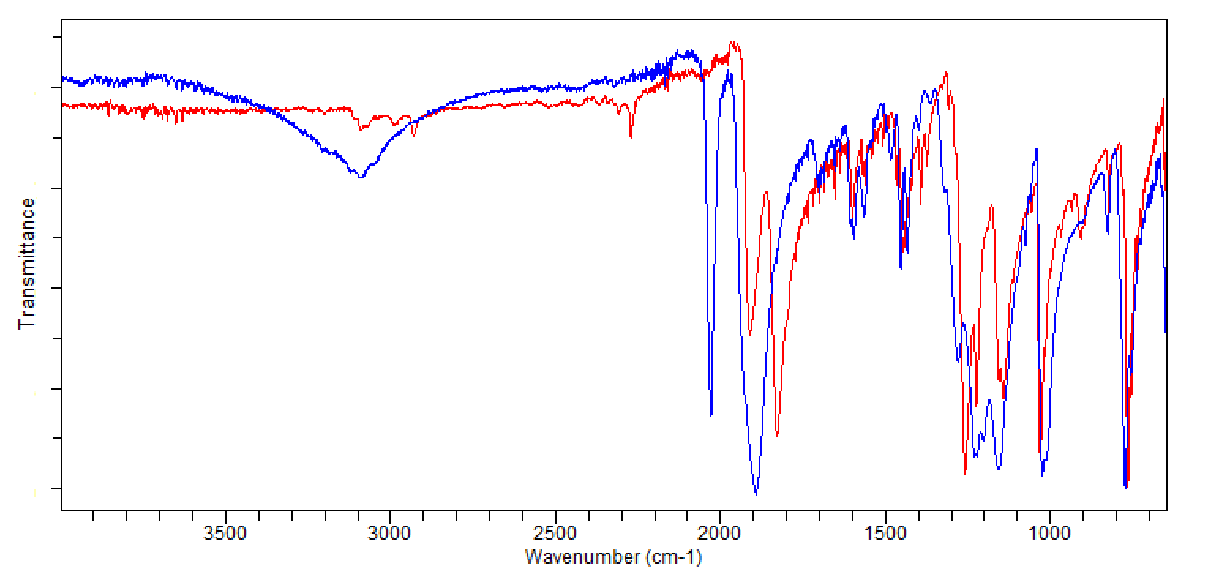
\includegraphics[clip=true, width=\textwidth, keepaspectratio]{images/ftir7and8.eps}
 \caption[FTIR Spectra for complexes \textbf{2.7} and \textbf{2.8}]{FTIR Spectra for complexes \textbf{2.7} (blue) and \textbf{2.8} (red).}
 \label{fig.ir78}
\end{figure}

\FloatBarrier
%----------------------------------------------------------------------
\subsection{Photophysical Properties}
%----------------------------------------------------------------------

A striking observation upon the conversion of the bidentate species into the terdentate complexes is that these new compounds have a substantially darker colour that reflects a significant change in the photophysical properties. This effect was investigated using a combination of UV-visible spectroscopy and \gls{ac.dft} modelling. Spectra were collected on a Agilent Cary 5000 UV-Vis-NIR Spectrophotometer. The stronger absorbance of the terdentate complexes compared to the bidentate precursors is evident in the UV-Vis spectra of these species, and is presented in \autoref{fig.uvvisbids} and \autoref{fig.uvvisters}. These spectra were obtained in \gls{ac.dmso} with approximate concentrations of 0.01 mM for bidentate, and an order of magnitude lower (0.001 mM) for the terdentate analogues. The terdentate complexes have more intense absorbance for higher energy ligand UV-based $\pi$-$\pi^\ast$ transitions (\textless 400~nm) and certainly a richer visible absorption profile that involve the \textit{d}-$\pi^\ast$ transitions. These features are responsible for the colour change observed.

\begin{figure}[!htb]
\centering
 \includegraphics[clip=true, width=120mm]{images/bidentateuvvis.eps}
 \caption[UV-Vis spectra for compounds \textbf{2.1}, \textbf{2.3}, \textbf{2.5}, and \textbf{2.7}]{UV-Vis spectra for compounds \textbf{2.1} (blue), \textbf{2.3} (green), \textbf{2.5} (red), and \textbf{2.7} (orange) at 0.01~mM concentration}
 \label{fig.uvvisbids}
\end{figure}

\begin{figure}[!htb]
\centering
 \includegraphics[clip=true, width=120mm]{images/terdentateuvvis.eps}
 \caption[UV-Vis spectra for compounds \textbf{2.2}, \textbf{2.4}, \textbf{2.6}, and \textbf{2.8}]{UV-Vis spectra for compounds \textbf{2.2} (blue), \textbf{2.4} (green), \textbf{2.6} (red), and \textbf{2.8} (orange) at 0.001~mM concentration}
 \label{fig.uvvisters}
\end{figure} 

The UV-Vis spectra were modelled using \gls{ac.tddft} computations within Gaussian 09, using the B3LYP functional with the LanL2DZ basis set and effective core potentials for the rhenium atom, and the TZVP basis set for all lighter atoms. Such functional and basis set choices are common within organometallic literature. Solvent was simulated using the integral equation formalized variant of the \gls{ac.pcm} solvation model, with DMSO as the solvent. 

The resulting computed spectra were excellent matches to the experimental spectra. The similarity of the spectra between the bidentate species and as well as the terdentate species indicates that parallel electronic transitions appear within these two groups. Specifics will be discussed for the chloro compounds, \textbf{2.1} and \textbf{2.2}, but strong parallels exist for all species. Plots of experimental and computational data for these two complexes are presented in \autoref{fig.uvvisbidec} and \autoref{fig.uvvisterec}, respectively.

\begin{figure}[!htb]
 \centering
  \includegraphics[clip=true, width=120mm, height=120mm, keepaspectratio]{images/uvvisbidec.eps}
 \caption[Plots of the experimental and computed UV-Vis spectra for compound \textbf{2.1}]{Plots of the experimental and computed UV-Vis spectra for compound \textbf{2.1}. The blue curve shows experimental result.The red vertical lines show the calculated transitions and relative intensities from the \gls{ac.tddft} calculations, while the red curve shows the Gauss convolution with peak width at half height of 0.250 eV.}
 \label{fig.uvvisbidec}
\end{figure}

\begin{figure}[!htb]
 \centering
  \includegraphics[clip=true, width=120mm, height=120mm, keepaspectratio]{images/uvvisterec.eps}
 \caption[Plots of the experimental and computed UV-Vis spectra for compound \textbf{2.2}]{Plots of the experimental and computed UV-Vis spectra for compound \textbf{2.2}.  The blue curve shows experimental result.The red vertical lines show the calculated transitions and relative intensities from the \gls{ac.tddft} calculations, while the red curve shows the Gauss convolution with peak width at half height of 0.250 eV.}
 \label{fig.uvvisterec}
\end{figure}

Common to all bidentate compounds were peaks at wavelengths of 315-320~nm, and peak shoulders near 350-375~nm (\autoref{fig.uvvisbids}). In the case of \textbf{2.1}, the computational results suggest that the experimental band centred at $\lambda$ = 315-320~nm (31750-31250~\ce{cm^{-1}}) primarily arises from two electronic transitions. The first is from HOMO-3 to LUMO, a $\pi$-$\pi^\ast$ transition, while the second major contribution is the excitation from HOMO to LUMO+2, which is a \textit{d}-$\pi^\ast$ transition. The \gls{ac.tddft} calculations suggest that the experimental band centred at $\lambda$ = 370~nm (27030~\ce{cm^{-1}}) corresponds to a calculated transition at approximately 400~nm, that is a \textit{d}-$\pi^\ast$ (HOMO-1 to LUMO) absorbance. Computed plots of molecular orbitals are included in \autoref{app.mos}, \nameref{app.mos}, \Cref{fig.mo21,fig.mo22,fig.mo23,fig.mo24,fig.mo25,fig.mo26,fig.mo27,fig.mo28}.

Like the bidentate samples, the spectra for the terdentate samples are quite similar to one another. In general, all of these species have much higher absorbance coefficients than their bidentate analogues; all contain long trailing absorptions across the wavelengths analysed. For terdentate complex \textbf{2.2}, the four experimentally observed UV-Vis absorptions observed are made up of six computed transitions. The computational model provided two equal and strong tranitions appearing at 308 and 325~nm to generate the experimental band centred at $\lambda$ = 330~nm (30300~\ce{cm^{-1}}). These arise from a transition from HOMO-5, to LUMO, a Cl lone-pair to terpy $\pi^\ast$ orbital absorption, and from HOMO-3 to LUMO, which is a ligand centred $\pi$-$\pi^\ast$ transition. All of the lower energy transitions are dominated by MLCT bands. The experimental band centered at $\lambda$ = 400~nm (25000~\ce{cm^{-1}}) arises from an electronic transition from HOMO to LUMO+3 which is \textit{d}-$\pi^\ast$ in nature. The absorbance centred at $\lambda$ = 460~nm (21740~\ce{cm^{-1}}) corresponds to two MLCT \textit{d}-$\pi^\ast$ transitions; HOMO-2 to LUMO and HOMO-1 to LUMO+1. Finally, the broad experimental band 680-715~nm (14700-14000~\ce{cm^{-1}}) arises from the electronic transition appearing at 718~nm, which is the excitation of a \textit{d}-electron in the Re-centered HOMO to the ligand $\pi^\ast$ LUMO.

\FloatBarrier
%----------------------------------------------------------------------
\subsection{Fluorescence}\label{ss.fluorescence}
%----------------------------------------------------------------------

Fluorescence data was collected for \textbf{2.1} and \textbf{2.2} using an Agilent Cary Eclipse Fluorescence Spectrophotometer, using a 5~nm excitation slit and emission slit, using excitation wavelengths selected to correspond to the centre of UV-Vis absorption bands. Data was collected for spectra in \gls{ac.dmf} to simulate the photocatalytic reaction environment (see \autoref{chap.co2}). Spectra are shown in \autoref{fig.fluoro} for \textbf{2.1} and \textbf{2.2} with their UV-Vis absorption spectra for comparison. Data is normalized to equil concentration for each sample in fluorescence and absorbance.

\begin{figure}[!htb]
 \centering
  \includegraphics[clip=true, width=140mm, height=100mm, keepaspectratio]{images/fluoro.eps}
 \caption[UV-Vis and fluorescence spectra for \textbf{2.1} and \textbf{2.2}]{UV-Vis and fluorescence spectra for \textbf{2.1} and \textbf{2.2}. Fluorescence of \textbf{2.1} from excitation of 373~nm (blue), excitation of \textbf{2.2} by 400~nm (red) and 470~nm (green) are shown, along with the absorption spectra of \textbf{2.1} (purple) and \textbf{2.2} (orange).}
 \label{fig.fluoro}
\end{figure}

Clearly the transformation from bidentate terpyridine to terdentate ligand has significant effect on the interactions of these Re compounds with visible light. While the terdentate sample is excited at various wavelengths (that should correspond to different absorption bands), the emission appears to be from one single band centred at ca.~485~nm. An emission band appears similarly in bidentate, centred at 480~nm, with a second, broad, weaker band appearing centred around 600~nm. The sharp peak observed at 420~nm is present in the \gls{ac.dmf} solvent blank as well.

Interestingly, emission is not seen with the naked eye with 400~nm excitation for the terdentate, while emission from the bidentate emission is a very strong, white light. This may be due to self-absorbance in the terdentate samples, emission of 490~nm is easily absorbed by the molecule. In the bidentate, no absorbance bands correspond with emission bands shown, these appear to the naked eye as a white emission.

\FloatBarrier
%----------------------------------------------------------------------
\section{Conclusions}
%----------------------------------------------------------------------

This work reported the first crystallographically authenticated rhenium(I) terpyridine terdentate complexes and thus expanded upon the prior limitations of Re coordination complexes. These terpyridine complexes are accessed via a simple, highly efficient, solid-state thermolysis pathway. They expand upon the known $\alpha$-diimine photophysical properties, with enhanced metal to ligand, \textit{d}-$\pi^\ast$ electronic transitions, occurring more frequently and with lower energy than in the associated bidentate compounds. These observations are supported by computational \gls{ac.tddft} results, affording an expanded understanding of the transition bands. Modification of the bidentate and terdentate species has been shown, the synthetic success of a triflate moiety should facilitate further development of reactivity and provides an opportunity for synthetic and catalytic studies.



 %"new geometry chemistry"
\cleardoublepage
%======================================================================
\chapter{Photocatalysis of \texorpdfstring{CO\textsubscript{2}}{CO2}}\label{chap.co2}
\markright{Photocatalysis of \texorpdfstring{CO\textsubscript{2}}{CO2}}
%======================================================================

%======================================================================
\section{Introduction}
%======================================================================

Only 6 years after \ce{Re^I} complexes using 2,2'-bipyridine were characterized, Hawecker, Lehn, and Ziessel showed the effectiveness of the compound for the photocatalytic reduction of \ce{CO2}\autocite{hawecker1983}. Since then, many have shown the efficacy of a wide range of $\alpha$-diimino complexes for the reaction\autocite{hawecker1986, kurz2006, portenkirchner2014} and expansion of the systems to bimetallic complexes with ruthenium and osmium as electron transfer agents has produced a wide range of results\autocite{rossenaar1996, takeda2008, tamaki2013}. The mechanism of reduction has been subject of some debate: while mechanisms have been proposed since Lehn et. al. soon after their original publication\autocite{hawecker1986}, modifications have been submitted routinely over the past decades\autocite{hayashi2003, morris2009, takeda2008, grills2010, agarwal2011, agarwal2012a, agarwal2012b, keith2013}. The development of a novel terdentate geometry and the associated increase in photon absorption at lower energies of the catalyst warranted investigation of the \ce{CO2} reduction capabilities, having overcome the criticism of only utilizing high energy photons \autocite{kutal1985}. 

%======================================================================
\section{Photocatalytic Reactions with New Compounds}
%======================================================================

The photocatalytic cycle is, simply, a photon-induced \gls{ac.mlct}, followed by the extraction of an electron from a sacrificial reductant. This radical, negatively charged species sheds the anion, opening up a reaction site. Reaction between a \ce{CO2}, a proton (from the decomposition of the reductant or elsewhere), and the catalyst yields any number of \ce{CO}, \ce{H2O}, formate (\ce{HCO2-}), or carbonate (\ce{CO3H-}), depending on the mechanistic pathway. Further discussion and a proposal of a new mechanism geometry based on computational and experimental data can be read in \autoref{chap.mech}.

%----------------------------------------------------------------------
\subsection{Conditions}
%----------------------------------------------------------------------

Reaction conditions in use in literature have remained typically unchanged since the original papers. A mixture of \gls{ac.dmf} with either \gls{ac.teoa} or \gls{ac.tea} at a 5:1 ratio is used to make a 1.0 mM solution of catalyst, with `excess' (depending on reference, a 1.1 to 25 molar ratio) electrolyte salt (typically \ce{Et4NX} or \textit{t}-\ce{Bu4NX}, where X = halide from catalyst) added as a stabilizer. Solutions are degassed by bubbling of \ce{CO2} and a consistent headspace is left to form over the solution. The reaction is monitored via \gls{ac.gc} analysis of the headspace, using a HP gas chromatograph with a 15 m CARBONPLOT column with 0.320 mm inner diameter and 1.50 $\mu$m film in a 40~$^\circ$C oven. The instrument is fitted with a \gls{ac.tcd}, and, while using He as a carrier gas, is able to resolve \ce{CO} and \ce{CO2} completely.  

%----------------------------------------------------------------------
\subsection{Experimental Results}
%----------------------------------------------------------------------

Both bidentate and terdentate \ce{$\kappa$^n(terpy)Re(CO)_{5-n}X} (n=2, 3) \textbf{2.1} and \textbf{2.2} complexes show no activity for \ce{CO2} reduction. Modification of testing time, light source, product analysis methods, solvent, sacrificial reductant, pH, presence of electrolyte, presence of \ce{H2O}, or variation of anion (X=Cl, Br, OTf, CN) shows no change of this inactivity. Testing of \ce{$\kappa$^2(bipy)Re(CO)3Cl} under the same reaction and testing conditions shows production of approximately 6 mL \ce{CO} from \ce{CO2} (~20\% conversion) in 1 hour of photolysis with visible ($\lambda$ \textgreater 400 nm) light, verifying the method, isolating the catalyst as the ineffective species. 

%======================================================================
\subsection{Rationalization of Results}\label{ss.rationalization}
%======================================================================

The lack of reactivity of the \ce{$\kappa$^2(terpy)Re(CO)3X} motif of complexes contrasting to the activity of the originally published \ce{$\kappa$^2(bipy)Re(CO)3X} indicates significant influence of the ligand on the reaction. Kurz \textit{et al.} demonstrated the requirement for fluorescence for successful catalytic candidates\autocite{kurz2006}. The explanation for this is the requirement for a stable, long-lasting excited state, with lifetime greater than that of the timescale required for electron abstraction from the sacrificial amine. The observed fluorescence demonstrates the lack of non-radiative relaxation pathways, considered to be an analogue for the extended lifetime of the excited state. Sample \textbf{2.2} shows only poor fluorescence. While the complex is able to absorb light across the spectrum, and has \gls{ac.homo} to \gls{ac.lumo} transitions with high enough energy\footnote{Electrochemical reduction of \ce{CO2} in similar environments takes 1.7-2.1 V, equivalent to \gls{ac.homo}-\gls{ac.lumo} transitions from 590-750 nm\autocite{grills2014}.} for the catalyzed reduction of \ce{CO2} to \ce{CO}, it appears as if the catalysis is not initiated due to a short excited state lifetime. Fluorescence data presented in \autoref{chap.newchem}, at \autoref{ss.fluorescence} shows the lack of strong fluorescence in terdentate sample \textbf{2.2}.

Explanation for the lack of \ce{CO} production observed in the attempted photochemical reduction of \ce{CO2} by bidentate sample \textbf{2.1} and others must come from another solution. These samples are quite fluorescent, emission from the powder sample can be seen with the naked eye with simulation by a 405 nm laser pen under ambient light environments.  Other substituted bipyridine ligands are known to be active for photocatalytic reduction \autocite{hawecker1986, kurz2006}, identifying the most likely conflicting feature of the terpyridine ligand to be the pendant arm itself.

\begin{figure}[!htbp]
 \begin{center}
  \includegraphics[clip=true, keepaspectratio, width=80mm]{images/yellowred.eps}
 \end{center}
 \caption[A photograph of aged and fresh catalytic mixture.]{A photograph of fresh (left) and aged (right) catalyst mixtures, showing the change from yellow to red in 5 days.}
 \label{fig.yellowred}
\end{figure}

Importantly, two clues come from the reaction mixture: under intense visible light in the presence of \ce{CO2} the compound bleaches to a very faint yellow-green and colour does not return after storage in the dark, bubbling of new \ce{CO2}, or other manipulations. Secondly, a mixture of sacrificial amine, \gls{ac.dmf}, and catalyst \textbf{2.1} in ratios identical to what is required in the reaction mixture changes colour from a yellow to a deep red irreversibly after approximately 5 days at ambient temperature, as shown in \autoref{fig.yellowred}. 

The most likely cause for the bleaching of the solution is the disassociation of terpyridine ligand from the metal centre. The colours seen in the catalyst are all due to metal-ligand interaction, and the UV-Vis spectrum of free terpyridine in solution is located solely in the UV range ($\lambda$\textsuperscript{max}~$\approx$~285~nm)\autocite{martin1956}. The labilization can be a photoinduced process\autocite{zink2001}. 

\begin{figure}[!htbp]
 \begin{center}
  \includegraphics[clip=true, keepaspectratio, width=120mm]{images/yellowreduvvis.eps}
 \end{center}
 \caption[UV-Visible spectra of freshly prepared and aged catalyst mixture.]{UV-Visible spectra of freshly prepared and aged catalyst mixture. DMF, DMF-TEOA (5:1), and DMF-TEOA + \ce{Et4NCl} (1 mmol) are shown in black, blue and olive, respectively. Fresh catalyst is shown in yellow (1 mmol catalyst), orange (0.5 mmol) and green (0.25 mmol). Aged catalyst is shown in red (1 mmol) and purple (0.5 mmol)}
 \label{fig.reduvvis}
\end{figure}

The UV-visible specta was obtained for the red compound formed after 5 days of ageing, showing some distinctive modifications (see \autoref{fig.reduvvis}). A peak appears at ca.~560~nm, and the metal to ligand \textit{d}-$\pi^\ast$ peak at 470 nm is reduced. Additionally, absorption increases at energies above 310~nm, where the fresh catalyst has a valley at ca.~285~nm, none exists for the aged sample.

\begin{scheme}[!htb]
 \begin{center}
  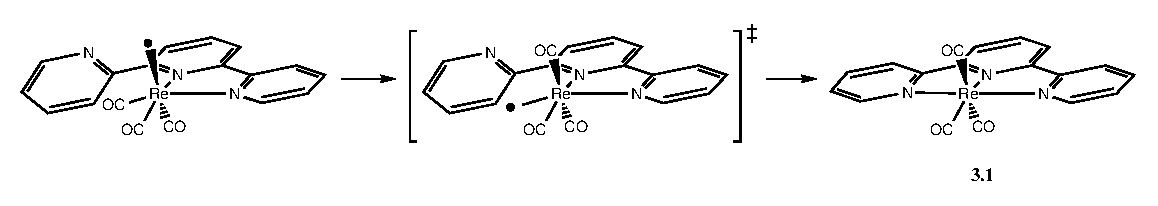
\includegraphics[clip=true, width=\textwidth, keepaspectratio]{images/tricarbscheme.eps}
 \end{center}
\caption[Reorganization from catalytic eximer to form \textbf{3.1}]{Formation of \textbf{3.1} from catalytic excimer via reorganization of carbonyls and chelation of the pendant arm.}
\label{scheme.tricarbonyl}
\end{scheme}

Other complexes may be formed that deactivate the catalyst, including the formation of a cationic tridentate tricarbonyl complex, seen in \autoref{scheme.tricarbonyl}. This species can be formed by the rearrangement of the carbonyl ligands from the \textit{fac} orientation to a \textit{mer}, migration of one carbonyl to the open site axial to the ligand achieves this reorganization. Once the \textit{mer} species is formed, the open site on the metal centre is oriented towards the pendant arm of the terpyridine ligand, coordination of that group to the metal centre results in compound \textbf{3.1}. The UV-Visible spectra of this species is not isolated, however, \gls{ac.dft} predicted UV-Vis is shown in \autoref{fig.uvvistricarb}, and compared to the experimental red product, these spectra do not correlate.

\begin{figure}[!htbp]
 \begin{center}
  \includegraphics[clip=true, keepaspectratio, width=120mm]{images/tricarbcatuvvisstruct.eps}
 \end{center}
 \caption[Structure and absorption spectra of proposed \ce{[$\kappa$^3-(terpy)-Re(CO)3]+}]{Computational structure (inset) and predicted UV-Vis absorption spectra of \ce{[$\kappa$^3-(terpy)-Re(CO)3]+} and experimental spectra of the aged catalytic mixture (orange).}
 \label{fig.uvvistricarb}
\end{figure}

Another deactivation product may be the formation of triethanolamine-catalyst adducts\autocite{morimoto2013}. In the presence of DMF, TEOA has been shown to bind to the open site of the excimer via the amine's oxygen atom. This is susceptible to insertion of \ce{CO2} to form a --\ce{OC(O)C}--\ce{CH2CH2N(CH2CH2OH)2} group. \Gls{ac.dft} studies on these two compounds suggest that they may be a coloured species, with predicted UV-Vis showing lower energy absorption than the catalyst itself (a red shift), demonstrated in \autoref{fig.ishitani}. The experimental red mixture UV-Vis spectra is overlaid, showing lack of correlation to the Ishitani compounds.

\begin{figure}[!htbp]
 \begin{center}
  
\includegraphics[clip=true, keepaspectratio, width=120mm]{images/ishitani.eps}
 \end{center}
\caption[Structure and absorption spectra of the catalyst-TEOA complex]{Computational structure (inset) and \gls{ac.dft} predicted UV-Vis absorption spectra for \textbf{2.1} (blue), the \gls{ac.teoa} complex proposed by Ishitani\autoref{fig.ishitani} (red), and experimental spectra of the aged catalytic mixture (green).}
\label{fig.ishitani}
\end{figure}

Neither the tricarbonyl terdentate nor the Ishitani complexes correlate to the observed spectra in \autoref{fig.reduvvis}. Identification of a compound solely by its spectra is not possible, however, some characteristics could be predicted. It is likely that there is a significant modification of the environment around the metal centre, previous observed electronic transitions that occur at that energy are due to metal \textit{d} to ligand $\pi^\ast$ interactions. Ligand $\pi$~to~$\pi^\ast$ transitions appear at much higher energy, and modification of those interactions could explain the lack of valleys observed in  the UV region (at 285~nm). Further determination of the complex is not possible with the collected data.

%======================================================================
\section{Conclusions}
%======================================================================

Experimental data shows the inactivity of these catalysts for photoreduction of \ce{CO2} under a range of experimental conditions. These same conditions show conversion using \ce{$\kappa$^2(bipy)Re(CO)3Cl} as the photoreductant, signifying the validity of experimental setup. The inactivity may be due to formation of inactive side-products or ligand labilization (for the case of bidentate catalyst) or due to the short excited state lifetime of the terdentate catalyst. 
 %"CO2 Chemistry" 
\cleardoublepage
%======================================================================
\chapter{Mechanism of \texorpdfstring{\ce{CO2}}{CO2} Reduction}\label{chap.mech}
\markright{Computational Study of the Mechanism of \texorpdfstring{\ce{CO2}}{CO2} Reduction}
%======================================================================

%======================================================================
\section{Introduction}
%======================================================================

Within three years of the appearance of the originally reported bipyridine rhenium (I) catalyst, experimental studies on the mechanism of the photocatalytic reduction of \ce{CO2} were available in the literature\autocite{hawecker1986}. Studies continue on the mechanism up to the present day\autocite{johnson1996, koike2002, takeda2008, smieja2012, machan2014, kou2014}, utilizing new investigative techniques as they become available to elucidate transition states and transient intermediates \textit{in situ}. 

Investigation includes the use of \gls{ac.dft} methods to elucidate geometries of intermediates and transition states for of the multi-step cycle. Transition metal catalysis is a non-trivial problem computationally, particularly when considering a metal from the lower period. These elements contain a large amount of electrons, many of which can be involved in non-covalent interactions with the ligands and catalyzed products. Solving for this complex system becomes non-trivial and computationally expensive. For this reason, no overview of the mechanism as investigated by \gls{ac.dft} methods has ever been made available in the literature. 

%======================================================================
\section{Mechanism Pathways}
%======================================================================

Prior work in the literature has proposed three general mechanistic pathways for the photoreduction of \ce{CO2}. In general, as seen in \autoref{fig.threepath}, these pathways result in the formation of \ce{CO} and \ce{H2O}, formate (\ce{HCO2-}), or carbonate (\ce{CO3H-}) anions. The formation of carbonate proceeds via the formation of a catalyst dimer over a molecule of \ce{CO2}, with the insertion of a second molecule of \ce{CO2} to produce the carbonate and a molecule of \ce{CO}. Production of formate occurs via insertion of \ce{CO2} to a rhenium hydride bond. The formation of \ce{CO} without carbonate or formate by-products occurs via the coordination of \ce{CO2} to an open site on the metal, followed by a double proton addition and the release of a molecule of \ce{H2O} prior to the loss of one of the four carbonyl groups to open up the axial site for halide re-coordination. This is essentially the \gls{ac.rwgsr}, wherein protons are made available from decomposition of the sacrificial amine instead of from decomposition of \ce{H2}\autocite{kalyanasundaram1978}. These three mechanistic pathways will be referred to as the `carbonate' mechanism, the `formate' mechanism, and the `water-gas shift' mechanism, respectively.

\begin{figure}[!htb]
 \begin{center}
  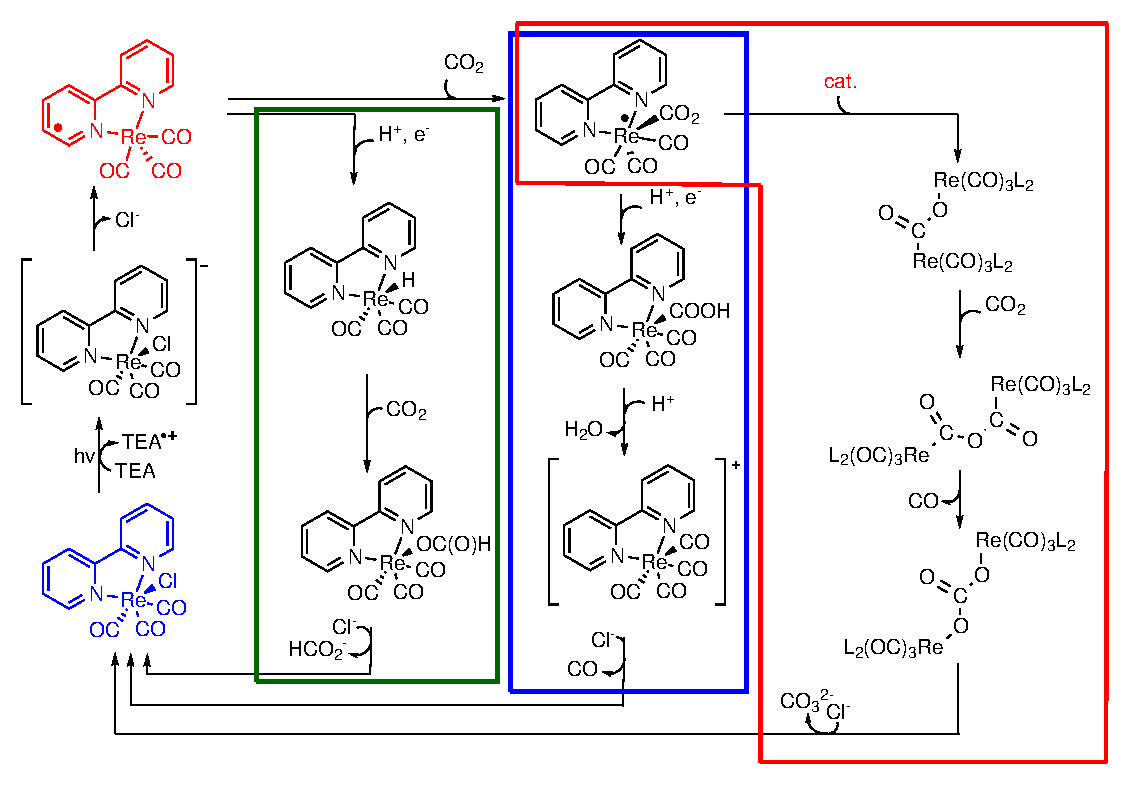
\includegraphics[clip=true, width=\textwidth, keepaspectratio]{images/threepaths.eps}
 \end{center}
\caption[Overview of mechanistic pathways]{An overview of the mechanistic pathways of photochemical \ce{CO2} reduction. Catalyst is shown in blue, and the excimer species in red}
\label{fig.threepath}
\end{figure} 

Each of the mechanistic pathways identified above in \autoref{fig.threepath} was studied, using \gls{ac.dft} methods. Structures (using 2,2'-bipyridine as the bidentate ligand, and triethylamine as the sacrificial reductant) were optimized to ground or transition states using TurboMole 6.5\autocite{turbomole, ahlrichs1989}, with the TPSS meta-GGA XC functional\autocite{tao2003}. The def2-TZVP basis set was used for all atoms\autocite{schafer1994, weigend2005}. The TurboMole program contains a number of optimizations to the original \gls{ac.dft} algorithms\autocite{haase1993, treutler1995, eichkorn1997, eichkorn1995, sierka2003, deglmann2004, weigend2002, vonarnim1998, ahlrichs2004}, decreasing the calculation time without compromising accuracy. Grimme's dispersion correction (version 3) was included in the calculations\autocite{grimme2010}. Intermediates and transition states were verified by frequency analysis\autocite{deglmann2004, deglmann2002, grimme2002}, with further verification of transition states by performing dynamic reaction coordinate calculations to determine the \glspl{ac.irc}. The effects of solvation was calculated using the Conductor-like Screening Model (COSMO) implemented in TurboMole\autocite{klamt1993}, which is a continuum solvation model implicitly surrounding the solute molecule. Code was developed to assist with managing the computational jobs (see \autoref{chap.turbocontrol}).

Many of the intermediates have been synthesized in various studies \autocite{shaver1992, gibson1998, gibson1999, gibson2003}, indicating their reasonable stability. While individual portions of the mechanism have been studied computationally in the past\autocite{agarwal2011, agarwal2012a, agarwal2012b}, no overarching study has compared methods relative to each other. Furthermore, while the formation of \ce{CO} with \ce{H2O} is the most anticipated pathway (due to the lack of formation of carbonate or formate in most studies), no literature pathway exists to explain the addition of \ce{CO2} to the open site of the radical catalytic species without a three body reaction step (catalyst, \ce{CO2} and \ce{H+} together) or without formate reorganization. Furthermore, no mechanism proposed thus far explains the \ce{^{12}CO} to \ce{^{13}CO} isotopic exchange demonstrated by Lehn's group in 1986\autocite{hawecker1986}. 

%---------------------------------------------------------------------
\subsection{Eximer Formation and Decomposition of the Sacrificial Amine}\label{ss.initiation}
%---------------------------------------------------------------------

All of the pathways require the formation of a common eximer, namely, the radical 17\textit{e}\textsuperscript{-} species (\autoref{fig.eximer}). This occurs through the absorption of an incident photon with enough energy to promote an electron from the metal d-orbital to the ligand $\pi^\ast$ orbitals in the ground state catalyst, \textbf{4.01}, forming the triplet \acrlong{ac.mlct} (3-MLCT) complex \textbf{4.01\textsuperscript{3MLCT}}. This excitation requires approximately 50 kcal/mol, sourced from absorbed light. The pseudo-oxidized, electron-deficient metal atom extracts an electron from the sacrificial amine present in the reaction solution to return to the \ce{Re^{I}} state (\textbf{4.02}). However, this complex is formally a radical anion, the halide (\textbf{4.04}) is lost to return to the neutral eximer species in solution, \textbf{4.03}. This extraction to form the radical anion catalyst and the radical cation amine is thermodynamically expensive in the gas phase, costing over 80 kcal/mol, but in solution phase in \gls{ac.dmf} releasing 5 kcal.The difference in energies demonstrates the importance of performing calculations in a simulated solution; steps that may have insurmountable energy barriers in the gas phase become possible once solvation is considered.

A slight uphill to dissociation of the chloride (15.44 kcal/mol in DMF) allows for the formation of the triplet 17~\textit{e}$^-$~excimer species \textbf{4.03}, from which the  mechanism pathways discussed in following subsections may diverge. It is important to note that some studies suggest the solvent coordinates with the excimer species \autocite{morris2009, kou2014}. This solvent coordination is expected to stabilize the excimer species prior to reaction with \ce{CO2} in solution\autocite{fujita2004}. However, this event has no bearing on the overall reaction energies, the coordination and subsequent loss of solvent is an energetically neutral occurrence and was not studied in detail.

\begin{figure}[!htb]
 \begin{center}
  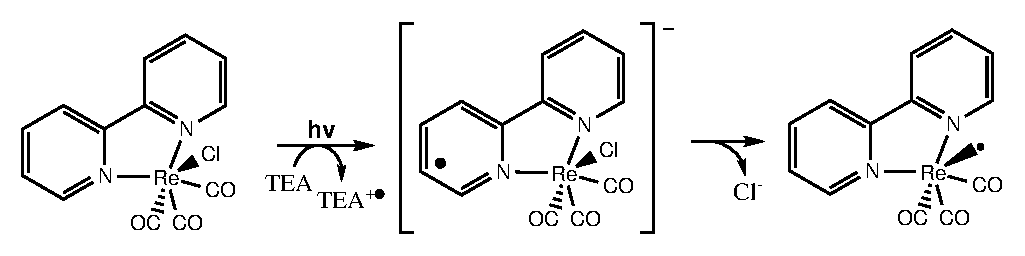
\includegraphics[clip=true, width=120mm, keepaspectratio]{images/eximer.eps}
 \end{center}
\caption{Formation of the eximer species via absorption of a photon and oxidation of the sacrificial amine.}
\label{fig.eximer}
\end{figure} 

The decomposition of the sacrificial amine was first identified by Kalyansundarem in 1978\autocite{kalyanasundaram1978}, and is summarized in \autoref{fig.decomp}. This work showed the route for decomposition of \gls{ac.teoa} but the mechanism for decomposition of \gls{ac.tea} is parallel. This decomposition is critical due to the protons it provides to the reaction mixture, and the presence of a simple second electron abstraction from the decomposition product. Upon absorption of a photon by the catalyst, the amine \textbf{4.05} is converted to the radical cationic species (\ce{Et3N^{+.}}, \textbf{4.06}). This undergoes a proton transfer to a second molecule of the sacrificial reductant. The transfer removes a proton from the $\alpha$ carbon, leaving it a neutral radical species (\textbf{4.07}). This is then able to react in the catalytic cycle to provide a second electron and form the ethene-diethylamino compound. Triethylammonia is produced as well (\textbf{4.08}), this is a proton source for the formate and water-gas shift mechanistic pathways. This step is slightly exothermic, with energy releases of 1 kcal/mol in gas phase, or nearly 3 kcal/mol in \gls{ac.dmf}.

\begin{figure}[!htb]
 \begin{center}
  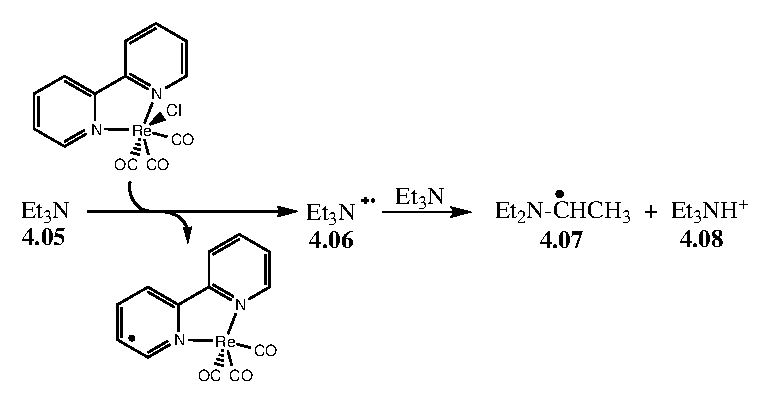
\includegraphics[clip=true, width=100mm, keepaspectratio]{images/reddecomp.eps}
 \end{center}
\caption{Decomposition pathway for the sacrificial amine.}
\label{fig.decomp}
\end{figure} 

Energies of \textbf{4.01} - \textbf{4.10}, and \textbf{4.26} in gas and solution phases (in \gls{ac.dmf}) is shown in \autoref{tab.supenergy}, along with the energy of solvation. Energies of each step of the reaction are listed in \autoref{tab.suprxn}. The values show a significant `uphill' series of steps requiring significant energy input. This energy is supplied by the incident photons; this process is a photocatalyzed activation. The reaction typically requires incident light of 400 nm energy\autocite{hawecker1983}, this significant energy input allows for the pathway to be followed.

% Table generated by Excel2LaTeX
\begin{table}[!htb]
\centering
 \begin{threeparttable}
  \caption[Gas phase and solvated energies for mechanism reactants and products]{Gas phase and solvated energies of mechanism reactants and products.}
    \begin{tabular}{llrrr}
    \toprule
    Molecule & Label & E (gas)\tnote{a} & E (solution)\tnote{b} & E (solvation)\tnote{c} \\
    \midrule
    Ground State & \textbf{4.01} & -1374.621419 & -1374.651099 & 18.62 \\
    3MLCT Complex & textbf{\textsuperscript{3}4.01\textsuperscript{MLCT}} & -1374.553193 & -1374.565998 & 8.04 \\
    Radical Anion & \textbf{4.02} & -1374.684002 & -1374.759190 & 47.18 \\
    Open Site Excimer & \textbf{4.03} & -914.3139376 & -914.3287245 & 9.28 \\
    Chlorine Anion & \textbf{4.04} & -460.2890817 & -460.4058583 & 73.28 \\
    Triethylamine (TEA) & \textbf{4.05} & -292.3051496 & -292.3854033 & 50.36 \\
    Radical Cation TEA & \textbf{4.06} & -292.3051496 & -292.3854033 & 50.36 \\
    Deprotonated TEA Radical & \textbf{4.07} & -291.9173706 & -291.9211226 & 2.35 \\
    Triethylammonia & \textbf{4.08} & -292.9552538 & -293.0382729 & 52.09 \\
    Carbon Dioxide & \textbf{4.09} & -188.6945676 & -188.6974631 & 1.82 \\
    Carbon Monoxide & \textbf{4.10} & -113.3744946 & -113.3754466 & 0.60 \\
    Diethylaminoethene & \textbf{4.26} & -291.3467768 & -291.3525868 & 3.64 \\
    \bottomrule
    \end{tabular}%
    \begin{tablenotes}
    \item [a] TPSS energy in hartrees.
    \item [b] TPSS energy in hartrees with COSMO solvation in DMF.
    \item [c] TPSS solvation energy in kcal/mol (E(gas) - E(solution)).
    \end{tablenotes}
  \label{tab.supenergy}%
 \end{threeparttable}
\end{table}%



% Table generated by Excel2LaTeX
\begin{table}[!htb]
\centering
 \begin{threeparttable}
  \caption{Energies for the reaction steps in the photoinduced excimer formation pathway}
    \begin{tabular}{r@{ $\rightarrow$ }lrr}
    \toprule
    \multicolumn{2}{c}{Steps} & Energy(gas)\tnote{a} & Energy(dmf)\tnote{b} \\
    \midrule
    \textbf{4.01} & \textbf{\textsuperscript{3}4.01\textsuperscript{MLCT}} & 42.81 & 53.40 \\
    \textbf{4.01\textsuperscript{3MLCT}} + \textbf{4.05} & \textbf{4.02} + \textbf{4.06} & 81.45 & -5.80 \\
    \textbf{4.02} & \textbf{4.03} + \textbf{4.04} & 50.82 & 15.44 \\
    \textbf{4.06} + \textbf{4.05} & \textbf{4.07} + \textbf{4.08} & -1.08 & -2.92 \\
    \bottomrule
    \end{tabular}%
    \begin{tablenotes}
    \item [a] TPSS energy in kcal/mol.
    \item [b] TPSS energy in kcal/mol with COSMO solvation in DMF.
    \end{tablenotes}
  \label{tab.suprxn}%
 \end{threeparttable}
\end{table}%




Geometries of the catalyst do not change significantly throughout this transformation, however, some changes occur signifying the change in electron localization. One metric analyzed in polyaromatic non-innocent ligand redox reactions is the bonding distance between aromatic rings \autocite{bokarev2014}. From ground state, through triplet MLCT complex to the excited radical, the C-C\textsubscript{(bpy)} distance decreases from 1.470 \r{A} to 1.425 \r{A} to 1.416 \r{A}. This 0.06 \r{A} decrease is noted in many previous experiments and calculations for anion radicals\autocite{bokarev2014, chisholm1981, castellaventura2000, gorerandall2009, irwin2010}. Other key bond lengths and angles include the ligand N-Re bonds and \ce{CO}-Re bonds, the addition and subtraction of electrons to and from the complex impact the bonding. As the reaction proceeds, for example, the calculated Re-N distance in solvated structures decreases from 2.18924 \r{A} in the ground state catalyst to 2.14212 \r{A} in the neutral radical excimer. Similarly, the distance from the metal to the axial carbonyl decreases from 1.91950 to 1.88746 \r{A} in the same circumstances. These changes are not significant, the bond order is unchanged across these distances, but bond modification of 0.05 \r{A} is large enough to demonstrate a change has occurred in the bonding around the metal. Subsequent steps in the mechanism demonstrate larger changes.

%---------------------------------------------------------------------
\subsection{The `Carbonate' Pathway}\label{ss.carbonate}
%---------------------------------------------------------------------

The carbonate pathway is shown in \autoref{fig.carbonate}, starting from the excimer species. This pathway has been studied in some detail in the literature, but never in a complete manner. Typical analysis consists of investigation from the formed \ce{CO2} linked dimer, through the release of \ce{CO}, terminating at the bicarbonate linked dimer. Studies typically build the dimer as a three-body reaction, or start with a \ce{Re\bond{-}Re} bound catalyst dimer and the insertion of \ce{CO2}. However, the formation of the  \ce{[L2Re(CO)3]2} is exceptionally slow in the presence of solvent, with a rate constant 8 orders of magnitude below\footnote{With the Thermodynamic Equilibrium formula $\Delta G^\circ = -RT ln(K)$, if $K \approx 10^7$, then $\Delta G^\circ \approx -40$ kJ/mol, $\approx$ -8 kcal/mol.} the solvent-stabilized radical \ce{$^\bullet$L2Re(CO)3(solv)} complex\autocite{fujita2004}. 

\begin{figure}[!ht]
 \begin{center}
  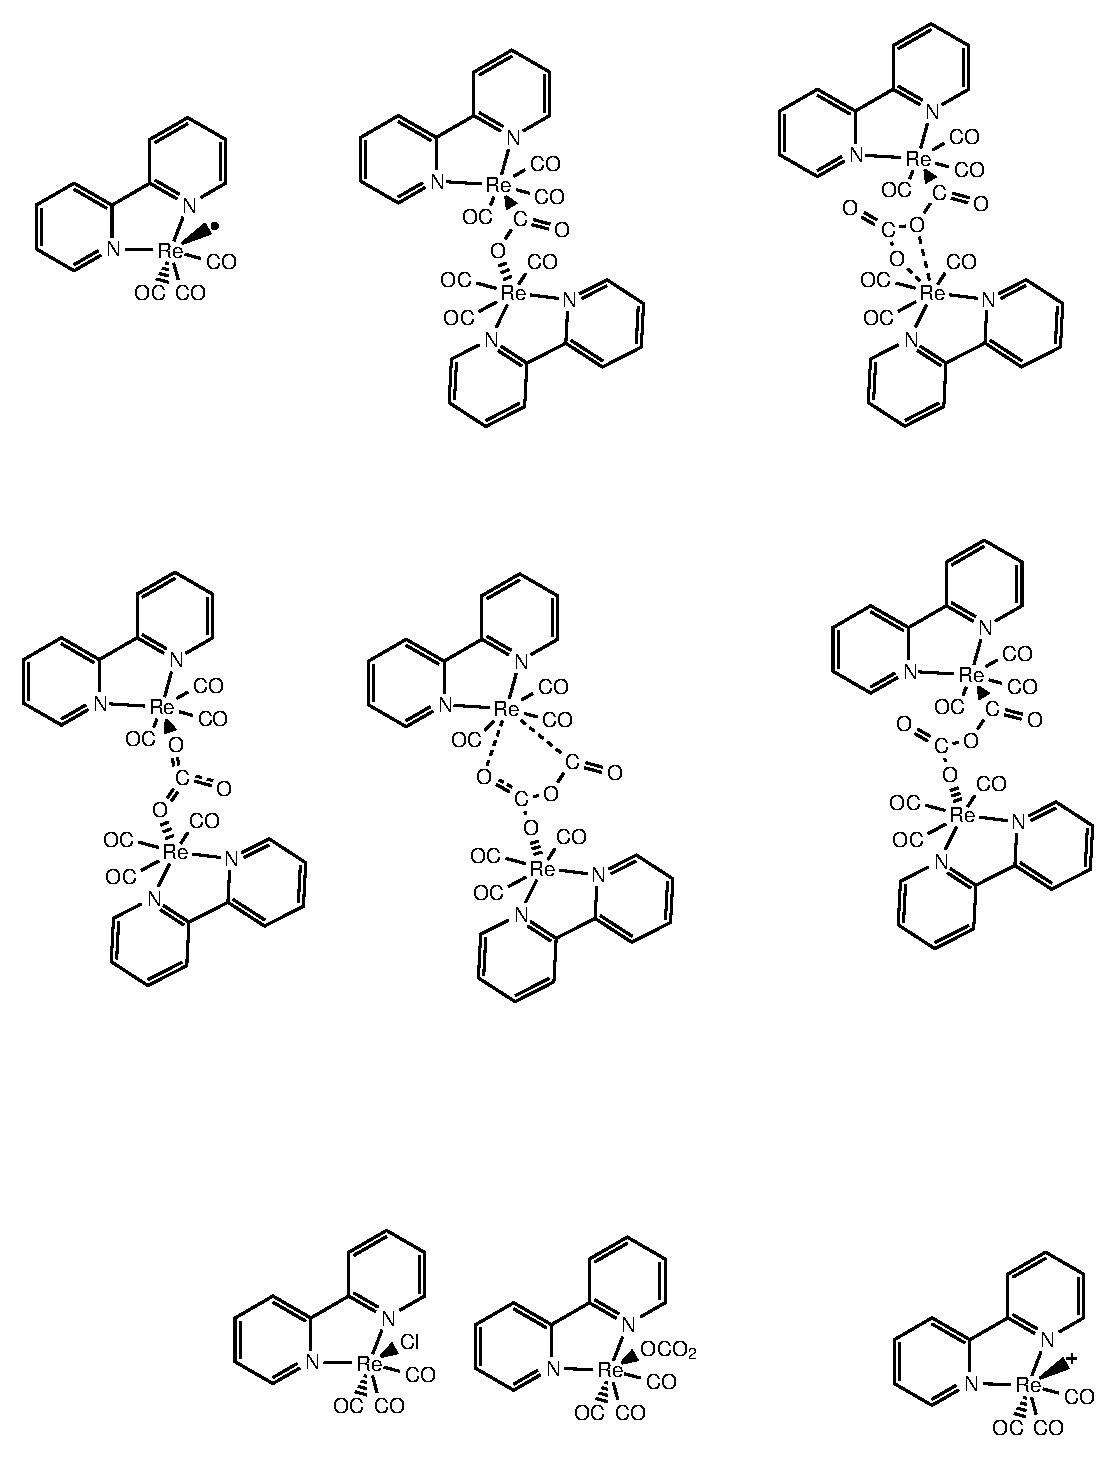
\includegraphics[clip=true, width=140mm, keepaspectratio]{images/carbonate.eps}
 \end{center}
\caption{The `carbonate' mechanistic pathway}
\label{fig.carbonate}
\end{figure} 

Energies of each of the compounds involved in this mechanism pathway are shown in \autoref{tab.carbenergy}, along with the energy of solvation. The full list of reaction energies are listed in \autoref{tab.carbrxn}.

% Table generated by Excel2LaTeX
\begin{table}[!htb]
\centering
 \begin{threeparttable}
  \caption[Gas phase and solvated energies for the `carbonate' mechanism]{Gas phase and solvated energies of compounds, transition states and intermediates in the `carbonate' mechanism}
    \begin{tabular}{llrrr}
    \toprule
    Molecule & Label & E (gas)\tnote{a} & E (solution)\tnote{b} & E (solvation)\tnote{c} \\
    \midrule
    \ce{CO2} Linked Dimer & 4.11 & -2017.373132 & -2017.412314 & 24.59 \\
    \ce{CO2} Addition TS & 4.12 & -2206.120721 & -2206.165017 & 27.80 \\
    \ce{C2O4} Linked Dimer & 4.13 & -2206.047558 & -2206.097328 & 31.23 \\
    5 Member Ringed Dimer TS & 4.14 & -2206.013925 & -2206.061531 & 29.87 \\
    \ce{CO3} Linked Dimer & 4.15 & -2092.678255 & -2092.725669 & 29.75 \\
    Bicarbonate Catalyst Cation & 4.16 & -1178.065153 & -1178.119717 & 34.24 \\
    Bicarbonate Anion & 4.17 & -264.4852375 & -264.4967144 & 7.20 \\
    Dimer Formation TS & 4.18 & -2017.434125 & -2017.47423151664 & 25.17 \\
    Bicarbonate Dianion & 4.19 & -263.7946209 & -264.1983931 & 253.37 \\
    Open Site Cation & 4.27 & -914.1064097 & -914.1872844 & 50.75 \\
    \bottomrule
    \end{tabular}%
    \begin{tablenotes}
    \item [a] TPSS SCF energy in hartrees.
    \item [b] TPSS SCF energy in hartrees with COSMO solvation in DMF.
    \item [c] TPSS solvation energy in kcal/mol (E(gas) - E(solution)).
    \end{tablenotes}
  \label{tab.carbenergy}%
 \end{threeparttable}
\end{table}%



\todo{check carbenergy values for 4.19}
% Table generated by Excel2LaTeX
\begin{table}[!htb]
\centering
 \begin{threeparttable}
  \caption{Energies for the reaction steps in the `formate' pathway}
    % Table generated by Excel2LaTeX from sheet 'Tex Charts
    \begin{tabular}{rrrr}
    \toprule
    Description & Steps & Energy(gas)\tnote{a} & Energy(dmf)\tnote{b} \\
    \midrule
    Formation of Radical Anion & 4.01, 4.05 \ce{->} 4.02, 4.06   & 124.261582 & 47.596907 \\
    Open site catalyst plus cl- & 4.02 \ce{->} 4.03, 4.04 & 50.816912 & 15.440887 \\
    Reconfiguration of TEA & 4.06, 4.05 \ce{->} 4.07, 4.08 & -1.077024 & -2.915901 \\
    \midrule
    Addition of CO2 to open site & 4.4   & -0.2501423 & 6.37310903 \\
    addition of second cat to CO2 & 4.5   & 118379.026 & 118375.044 \\
    Insertion of CO2 & 4.6   & \#VALUE! & -8.5491267 \\
    relaxation of co2 insertion & 4.7   & \#VALUE! & -0.6637971 \\
    rearrange to 4ring dimer & 4.8   & \#VALUE! & \#VALUE! \\
    relax to long & 4.9   & \#VALUE! & \#VALUE! \\
    rearrangement to 5ring dimer & 4.1   & \#VALUE! & 22.4628711 \\
    relax to final & 4.11  & \#VALUE! & -24.839557 \\
    break apart & 4.12  & 317.951051 & 262.714812 \\
    return to ground states & 4.13  & -613.91666 & -426.82371 \\
    \bottomrule
    \end{tabular}%
    \begin{tablenotes}
    \item [a] TPSS SCF energy in kcal/mol.
    \item [b] TPSS SCF energy in kcal/mol with COSMO solvation in DMF.
    \end{tablenotes}
  \label{tab.carbrxn}%
 \end{threeparttable}
\end{table}%


The mechanism begins with the addition of a \ce{CO2} molecule to the excimer, forming \textbf{4.11}. This is a very weakly bound species when solved in a simulated \gls{ac.dmf} environment; in the gas phase this transition complex will not solve. Energies for the gas phase for this compound are calculated as single point energies from the solvated structure. The \gls{ac.dmf} solved structure has a Re-C bond length of 2.50654 \r{A}, and O-C-O bonding angle of 142$^\circ$, when compared to the \ce{Re\bond{-}C} distances of rhenium carbonyls of \textit{ca}. 1.9 \r{A}, this is a very weak bond. The formation of this `bond' requires only 6.37 kcal/mol, the radical species is not satisfied with the addition of \ce{CO2} and requires further electron contribution to become more stable. This unstable complex is able to extract a hydrogen to continue with the formate pathway (see below \autoref{ss.formate}), or combine with a second molecule of the excimer to form a dimer \textbf{4.13}. This dimer formation is explicitly not favoured; although resolution of radical species is provided, the transformation via \textbf{4.12} is still \todo{numb} kcal/mol uphill in \gls{ac.dmf}. Explanation of this untenably large value may be the root of the choice in literature to utilize the Re-Re bound dimer species as the catalyst starting point, instead of the ground state. \todo{From this point onwards the reaction proceeds in achievable downhill steps, the formation of the dimer is the rate limiting step for the entire reaction pathway.} The quenching of the radical forms much stronger bonds between the metal atoms and the linking \ce{CO2}. The Re-C distance has shortened from the 2.50654 \r{A} seen in \textbf{4.11} to 2.25829 \r{A}. This is still longer than the Re-CO bonds, expected due to the lack of $\pi$ back-bonding observed with carbonyl ligands, however, it corresponds with similar published crystal structures of Re-C bond lenghts for sp\textsuperscript{2} carbons\autocite{lukehart1977}. The Re-O bond is 2.13 \r{A}, a value that remains constant for Re-O through the intermediates in the reaction pathway.

After the dimer \textbf{4.13} has been formed, a second molecule of \ce{CO2} is inserted via \textbf{4.14} to form the Re-C-O-C-O-Re complex \textbf{4.15} (see structures \textbf{4.12} - \textbf{4.17} in \autoref{fig.carbonatestruc}). This linker contains bonds from length 1.28 - 1.44 \r{A}, typical for sp\textsuperscript{2}-carbon oxygen bonds. Bond angles are typically just under the idealized 120$^\circ$ expected as well. Due to the linker, the catalyst ligand bipyridines have moved from a nearly co-planar geometry to a nearly perpendicular geometry. Re-C and Re-O bonds remain constant in length compared to \textbf{4.13}. Following the insertion of the second molecule of \ce{CO2}, internal rearrangements progress this complex through the release of a molecule of \ce{CO} and the formation of the bicarbonate byproduct. The formation of a 5 membered ring in the \textbf{4.16} transition state leads to the release of the \ce{CO} and the formation of a carbonate linked dimer, \textbf{4.17}, returning the catalyst ligands to a more co-planar orientation. The carbonate dimer species is left to decompose to a catalyst cation \textbf{4.20} with an open site, and the bicarbonate adduct \textbf{4.18}. This carbonate dianion may pick up a proton before or after the disassociation to the catalyst cationic species, resulting in the released of the bicarbonate species to solution (\textbf{4.19)} when the catalyst is returned to ground state \textbf{4.01} with addition of a chloride. 

\begin{figure}[!ht]
 \begin{center}
  \includegraphics[clip=true, width=120mm, keepaspectratio]{images/carbonatestruc.eps}
 \end{center}
\caption{DFT calculated structures for the `carbonate' mechanistic pathway}
\label{fig.carbonatestruc}
\end{figure} 

\todo{maybe take this out?}Some work done by Agarwal \textit{et. al.} provides an opportunity for a catalytic pathway with similar results requiring only one molecule of catalyst\autocite{agarwal2012a}. Instead of capping the loosely coordinated \ce{CO2} with the eximer, the radical is quenched with a hydride extraction from the sacrificial amine, much as in the pathway described in \autoref{ss.formate}. A second molecule of \ce{CO2} reacts with the acid, undergoing a series of reorganization and dissociation/re-association steps to produce the carbonate. The experimental data supporting this variation of the mechanism is not strong; further validation should be required for this mechanism variation to gain popularity in the literature. 

%---------------------------------------------------------------------
\subsection{The `Formate' Pathway}\label{ss.formate}
%---------------------------------------------------------------------
In comparison to the catalytic dimer formed in the carbonate pathway above, the formate formation occurs via a much simpler mechanism. The addition of a proton to the open site axial to the ligand occurs via the simultaneous electron and proton transfer from a by-product of the reduction of the amine. \ce{CO2} inserts into this metal hydride bond, resulting in a metal-oxide bond, with the formate anion. Separation of the weak metal-oxygen bond allows for the reinsertion of the halide to the cationic metal centre. 

\begin{figure}[!htb]
 \begin{center}
  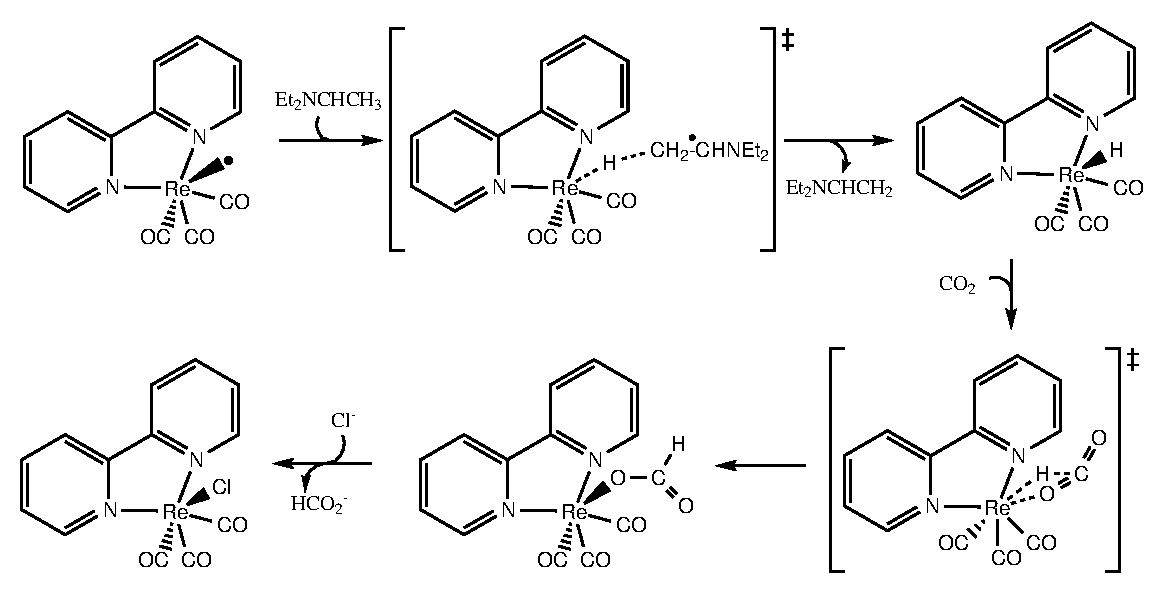
\includegraphics[clip=true, width=\textwidth, keepaspectratio]{images/formate.eps}
 \end{center}
\caption{The `formate' mechanistic pathway}
\label{fig.formate}
\end{figure} 

Energies of each of the compounds involved in this mechanism pathway are shown in \autoref{tab.formenergy}, along with the energy of solvation.

% Table generated by Excel2LaTeX
\begin{table}[!htb]
\centering
 \begin{threeparttable}
  \caption[Gas phase and solvated energies for the `formate' mechanism]{Gas phase and solvated energies of compounds, transition states and intermediates in the `formate' mechanism}
    \begin{tabular}{llrrr}
    \toprule
    Molecule & Label & E (gas)\tnote{a} & E (solution)\tnote{b} & E (solvation)\tnote{c} \\
    \midrule
    Proton Transfer TS & 4.21  & -1206.302997 & -1206.32707 & 15.10 \\
    Catalyst Hydride & 4.22  & -914.9204746 & -914.9448354 & 15.29 \\
    \ce{CO2} Insertion TS & 4.23  & -1103.581201 & -1103.619960 & 24.32 \\
    Catalyst Formate & 4.24  & -1103.635283 & -1103.665628 & 19.04 \\
    Formate Anion & 4.25 & -189.3051464 & -189.4151284 & 69.01 \\
    Open Site Cation & 4.27  & -914.1064097 & -914.1872844 & 50.75 \\
    \bottomrule
    \end{tabular}%
    \begin{tablenotes}
    \item [a] TPSS SCF energy in hartrees.
    \item [b] TPSS SCF energy in hartrees with COSMO solvation in DMF.
    \item [c] TPSS solvation energy in kcal/mol (E(gas) - E(solution)).
    \end{tablenotes}
  \label{tab.formenergy}%
 \end{threeparttable}
\end{table}%



% Table generated by Excel2LaTeX
\begin{table}[!htb]
\centering
 \begin{threeparttable}
  \caption{Energies for the reaction steps in the `formate' pathway}
    % Table generated by Excel2LaTeX from sheet 'Tex Charts
    \begin{tabular}{rrrr}
    \toprule
    Description & Steps & Energy(gas)\tnote{a} & Energy(dmf)\tnote{b} \\
    \midrule
    Formation of Radical Anion & 1.1   & -39.271301 & -67.827267 \\
    Open site catalyst plus cl- & 1.2   & 50.8169125 & 15.4408871 \\
    Reconfiguration of TEA & 1.3   & -164.60991 & -118.34007 \\
    \midrule
    Hydride Extraction & 1.4   & 4.09794743 & -9.8319638 \\
    Removal of TEA & 1.5   & -26.652434 & -20.021496 \\
    Insertion of CO2 & 1.6   & 21.2356096 & 14.0177223 \\
    recoordination & 1.7   & -33.936535 & -28.657394 \\
    dissasotiation of HCO2- & 1.8   & 140.389052 & 39.6680755 \\
    Reformation of Catalyst & 1.9   & -141.76995 & -36.367745 \\
    \bottomrule
    \end{tabular}%
    \begin{tablenotes}
    \item [a] TPSS SCF energy in kcal/mol.
    \item [b] TPSS SCF energy in kcal/mol with COSMO solvation in DMF.
    \end{tablenotes}
  \label{tab.formrxn}%
 \end{threeparttable}
\end{table}%



After formation of the excimer \textbf{4.03}, the radical species extracts a hydrogen atom from the oxidized chain of the sacrificial amine \textbf{4.07} in transition state \textbf{4.21} \todo{fix numbering see carbonate}, a step with a barrier of 4.16 kcal/mol in the gas phase, and is favoured by nearly 10 kcal/mol in \gls{ac.dmf}. The sacrificial amine involved in this step had previously had one proton extracted by another molecule of the amine in a proton exchange step (see \autoref{ss.initiation}), resulting in a neutral radical. Extraction of the proton and electron pair allows for the formation of an ethene arm, completing the decomposition of the amine to the final neutral, singlet molecule \textbf{4.26}. Relaxation of this transition state results in the hydrogen extraction from the radical species, yielding the formation of the hydride complex \textbf{4.22}.

Some attempt was made at performing the reaction along alternative pathways. While direct $\sigma$ bonding from a metal to an oxygen atom in the \ce{CO2} molecule (as $\eta^1$-OCO) has been observed in a few systems (including photoreduction of \ce{CO2})\autocite{lee2001, mauser2001, souter1997}, this geometry is rare\autocite{castrorodriguez2004, cokoja2011, gibson1996}. Attempts to coordinate \ce{CO2} in an $\eta^1$ geometry failed to converge both in gas and solution phase, \ce{CO2} was ejected from the complex, resulting in the excimer species \textbf{4.03}. Binding of \ce{CO2} to the metal through $\pi$ coordination of the C=O bond is more common\autocite{cokoja2011, gibson1996}, but these structures failed to solve in the current \gls{ac.dft} system as well, typically via the dissociation of the \ce{CO2}.

This hydride complex is able to insert a molecule of \ce{CO2} into the metal-hydrogen bond, in transition step \textbf{4.23}. \ce{CO2} insertion to metal hydrides is commonly observed, leading mechanisms in \ce{CO2} reduction in ruthenium systems employ this addition\autocite{creutz2007}. Rhenium I hydrides are very rare, appearing only in literature in the discussion of the photocatalytic mechanism. The Re-H bond length is 1.76 \r{A}, compared to the length of the Re-Cl bond from the ground state \textbf{4.01} species of 2.51 \r{A}. This bond length difference reflects the observations on anion change from Cl to Br, the anion size is the critical factor in this variation. When a molecule of \ce{CO2} approaches, the transition state of a pseudo-septacoordinate species \textbf{4.2?} forms. The formation is expensive, at just over 14 kcal/mol. The Re-H bond increases in length to 2.16 \r{A}, the Re-O bond is 2.88 \r{A}, and the O-Re-H angle is very tight, at only 45.3 $^\circ$. This step completes with 28.66 kcal/mol energy release to form the formato anion complex \textbf{4.2?}. 

The formato anion \textbf{4.2?} contains a Re-O bond of 2.15 \r{A}, consistent with previously discussed rhenium - oxygen bonds. This formate dissociates with a chloride addition, the exchange is endothermic by less than 3 kcal/mol. This counterion switch is likely more favoured in the real solution, the presence of excess molar equivalents of an electrolyte such as tetraethylammoniumchloride ensures a surplus of chloride anions are in solution and force the conversion by entralpic means. Further reactions of the formato anion in solution are not investigated, but the anion likely remains deprotonated in the slightly basic environment. 

\FloatBarrier

%---------------------------------------------------------------------
\subsection{The `Water-Gas Shift' Pathway}\label{ss.watergas}
%---------------------------------------------------------------------
The water-gas shift mechanism involves the addition of two protons from the reductant to a \ce{CO2} molecule bound to the metal centre. The first proton addition yields an acid species, this is dehydrated via the second addition of a proton and the release of one molecule of \ce{H2O}. The resulting tetracarbonyl cationic species is able then to release an axial carbonyl to return to the ground state. While any of the carbonyl groups could be labile, the carbonyl at the axial position is the one actively replaced by the halide to return to the starting catalyst\autocite{shaver1992}. 

\begin{figure}[!htb]
 \begin{center}
  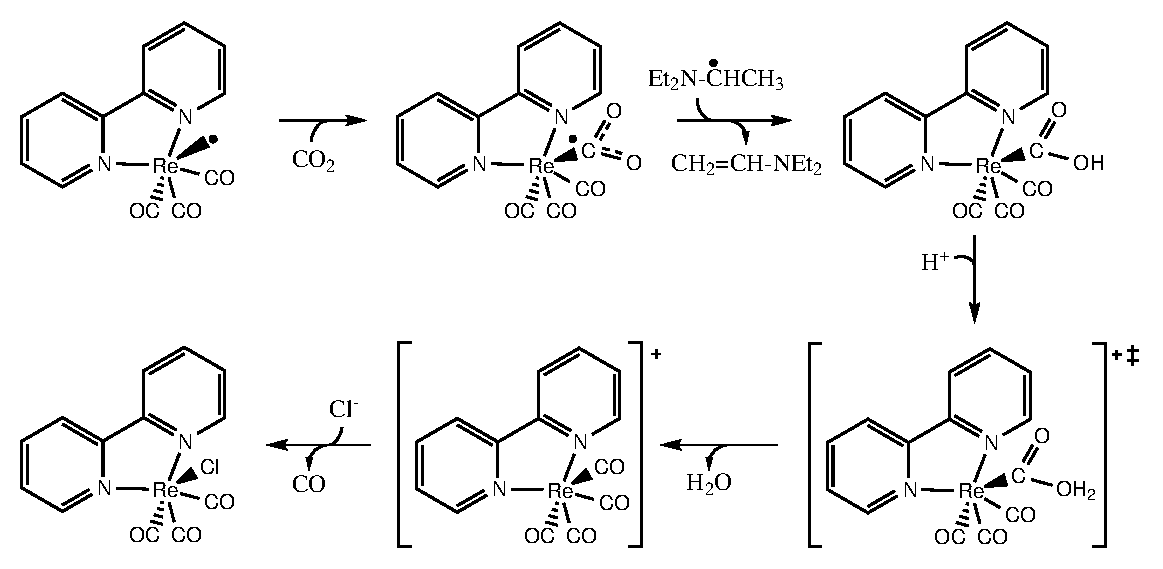
\includegraphics[clip=true, width=\textwidth, keepaspectratio]{images/watergas.eps}
 \end{center}
\caption{The `water-gas shift' mechanistic pathway}
\label{fig.watergas}
\end{figure} 

Energies of each of the compounds involved in this mechanism pathway are shown in \autoref{tab.wgsenergy}, along with the energy of solvation.

% Table generated by Excel2LaTeX
\begin{table}[!htb]
\centering
 \begin{threeparttable}
  \caption[Gas phase and solvated energies for the `water-gas shift' mechanism]{Gas phase and solvated energies of compounds, transition states and intermediates in the `water-gas shift' mechanism}
    \begin{tabular}{llrrr}
    \toprule
    Molecule & Label & E (gas)\tnote{a} & E (solution)\tnote{b} & E (solvation)\tnote{c} \\
    \midrule
    Catalyst-\ce{CO2} (Axial) & 4.31  & -1103.008904 & -1103.016031 & 4.47 \\
    Catalyst-\ce{CO2H} (Axial) & 4.32  & -1103.610331 & -1103.640451 & 18.90 \\
    \ce{H2O} Dissociation (Axial) TS & 4.33  & -1104.018352 & -1104.093313 & 47.04 \\
    Catalyst-\ce{CO2} (Equatorial) & 4.34  & -1102.963633 & -1102.992198 & 17.92 \\
    Catalyst-\ce{CO2H} (Equatorial) & 4.35  & -1103.597572 & -1103.625739 & 17.68 \\
    \ce{H2O} Dissociation (Equatorial) TS & 4.36  & -1104.016156 & -1104.093644 & 48.62 \\
    Water & 4.37 & -76.46413339 & -76.47581393 & 7.33 \\
    Tetracarbonyl Catalyst Cation & 4.38  & -1027.546073 & -1027.619412 & 46.02 \\
    H Transfer to Axial \ce{CO2} TS & 4.39  & -1394.981543 & -1395.011603 & 18.86 \\
    H Transfer to Equatorial \ce{CO2} TS & 4.40  & -1394.938949 & -1394.991623 & 33.05 \\
    Catalyst with Migrated Open Site & 4.41  & -914.2766988 & -914.2972247 & 12.88 \\
    \bottomrule
    \end{tabular}%
    \begin{tablenotes}
    \item [a] TPSS SCF energy in hartrees.
    \item [b] TPSS SCF energy in hartrees with COSMO solvation in DMF.
    \item [c] TPSS solvation energy in kcal/mol (E(gas) - E(solution)).
    \end{tablenotes}
  \label{tab.wgsenergy}%
 \end{threeparttable}
\end{table}%



% Table generated by Excel2LaTeX
\begin{table}[!htb]
\centering
 \begin{threeparttable}
  \caption{Energies for the reaction steps in the `formate' pathway}
    \begin{tabular}{rrrr}
    \toprule
    Description & Steps & Energy(gas)\tnote{a} & Energy(dmf)\tnote{b} \\
    \midrule
    Formation of Radical Anion & 2.1   & -39.271301 & -67.827267 \\
    Open site catalyst plus cl- & 2.2   & 50.8169125 & 15.4408871 \\
    Reconfiguration of TEA & 2.3   & -164.60991 & -118.34007 \\
    \midrule
    migration of open site? & 2.4   & 23.3674263 & 19.7662463 \\
    Addition of CO2 to open site & 2.5   & 4.78987184 & 1.56207334 \\
    H transfer to CO2 & 2.6   & -61.998066 & -35.596525 \\
    CO2H planar relaxation & 2.7   & 22.2489536 & -5.1943905 \\
    COOH2 ts & 2.8   & 144.908364 & 116.570584 \\
    CO4 + and water & 2.9   & 4.10436095 & -1.4970678 \\
    dissassotiation of CO & 2.10  & 40.893777 & 35.5673996 \\
    Reformation of Catalyst & 2.11  & -141.76995 & -36.367745 \\
    \bottomrule
    \end{tabular}%
    \begin{tablenotes}
    \item [a] TPSS SCF energy in kcal/mol.
    \item [b] TPSS SCF energy in kcal/mol with COSMO solvation in DMF.
    \end{tablenotes}
  \label{tab.wgsrxn}%
 \end{threeparttable}
\end{table}%




This mechanistic pathway it thought to start by the same addition of CO2 that is seen in the carbonate mechanism (see \autoref{ss.carbonate}, forming \textbf{4.11}. \todo{check compound numbers} As before, the complex is only weakly coordinated, and requires solvation effects to solve computationally. The added \ce{CO2} is able to extract a hydrogen from the previously-reduced sacrificial amine \textbf{4.07}, allowing the completion of the ethene formation \textbf{4.26}. The newly formed acid species \textbf{4.32} dehydrates in the presence of a second proton (via \textbf{4.33}) to form water \textbf{4.37} and the tetracarbonyl cationic species \textbf{4.38}. 

Typically, this reaction had been thought to proceed on the axial site of the catalyst, mirroring the pathways discussed above. However, due to the ease of migration of the carbonyl groups, it is proposed that the `water-gas shift' mechanism does not occur entirely axial to the ligand, but begins with coordination of a \ce{CO2} molecule in between the \textit{facial}-\ce{CO} ligands, forcing a carbonyl to the axial position \textbf{4.34}. This \ce{CO2} bound in the plane of the ligand then undergoes hydrogen addition and dehydration to produce a molecule of \ce{H2O}, continuing as before. While any of the carbonyl groups could be labile, the carbonyl at the axial position is replaced by the halide to return to the starting catalyst\autocite{shaver1992}. 

This newly proposed mechanism provides a solution to a previously unexplained phenomenon. The exchange of carbonyl groups on the catalyst for \ce{^{13}CO} when using \ce{^{13}CO2} in the photoreduction is documented as early as Hawecker \textit{et al}\autocite{hawecker1986}. It was shown that complete exchange occurs with very few catalytic turnovers. Furthermore, Koike \textit{et al}. demonstrated that photochemical ligand substitution occurs at only axial sites relative to the $\alpha$-imino ligand\autocite{koike2002}, no exchange occurs at the equatorial site, nor do the \textit{fac}-\ce{(^{12}CO)2^{13}CO} reorganize to shift the \ce{^{13}CO} to the equatorial position in the timeframe of the reaction. Thus the isotopic exchange does not proceed by independent uptake of product \ce{^{13}CO}, but in fact the conversion to the \ce{^{13}CO} complex must occur via the reduction mechanism. 

\FloatBarrier

%---------------------------------------------------------------------
\subsection{Consequences From \texorpdfstring{\ce{$\kappa$^2}}{Bidentate} Terpyridine Complex Inactivity}
%---------------------------------------------------------------------

The lack of reactivity of the \ce{$\kappa$^2(terpy)Re(CO)3X} motif of complexes contrasting to the activity of the originally published \ce{$\kappa$^2(bipy)Re(CO)3X} indicates significant influence of the ligand on the mechanism. While the terdentate complex can be rationalized to be inactive due to its short-lived excited state (as seen in \autoref{chap.newchem}) \autocite{shavaleev2004}, this explanation does not suffice for the fluorescing bidentate complex. Other substituted bipyridine ligands are known to be active for photocatalytic reduction \autocite{hawecker1986, kurz2006}, identifying the most likely conflicting feature of the terpyridine ligand to be the pendant arm, and its availability for chelation to the metal centre. While in the radical eximer form, the chelation site is sterically blocked by one of the three carbonyl groups. However, reorganization of the substituent carbonyls from a \textit{facial} orientation to a \textit{meridional} could allow for the free pyridine to form the metal-ligand bond, resulting in compound (X).\todo{What is X}

% Table generated by Excel2LaTeX
\begin{table}[!htb]
\centering
 \begin{threeparttable}
  \caption{Energies for the reaction steps in the `formate' pathway}
    % Table generated by Excel2LaTeX from sheet 'Tex Charts
    \begin{tabular}{rrrr}
    \toprule
    Description & Steps & Energy(gas)\tnote{a} & Energy(dmf)\tnote{b} \\
    \midrule
    Formation of Radical Anion & 4.01, 4.05 \ce{->} 4.02, 4.06   & 124.261582 & 47.596907 \\
    Open site catalyst plus cl- & 4.02 \ce{->} 4.03, 4.04 & 50.816912 & 15.440887 \\
    Reconfiguration of TEA & 4.06, 4.05 \ce{->} 4.07, 4.08 & -1.077024 & -2.915901 \\
    \midrule
    Addition of CO2 to open site & 3.4   & -0.2501423 & 6.37310903 \\
    H transfer to CO2 & 3.5   & -19.133571 & -33.878805 \\
    CO2H axial relaxation & 3.6   & -0.2145456 & -1.1883574 \\
    COOH2 ts & 3.7   & 151.907871 & 125.579781 \\
    CO4 + and water & 3.8   & 5.1112987 & -1.2748062 \\
    dissassotiation of CO & 3.9   & 40.893777 & 35.5673996 \\
    Reformation of Catalyst & 3.10  & -141.76995 & -36.367745 \\
    \bottomrule
    \end{tabular}%
    \begin{tablenotes}
    \item [a] TPSS SCF energy in kcal/mol.
    \item [b] TPSS SCF energy in kcal/mol with COSMO solvation in DMF.
    \end{tablenotes}
  \label{tab.siderxn}%
 \end{threeparttable}
\end{table}%




%======================================================================
\section{Comparison Between Mechanistic Pathways} \label{sec.compare}
%======================================================================

Previous studies in literature had only analyzed one of the mechanistic pathways (or a subsection thereof), without a fuller analysis of the competitiveness of each pathway relative to the others. Discussion on the tenability of each potential pathway relied on the \textit{in situ} observation of intermediates or transition states, the success (or lack thereof) of synthesis of the intermediates, and the relative production of by-products in the mechanistic trials. 

The overall energies for each of the mechanistic pathways shown in \autoref{fig.threepath} are shown in \autoref{fig.threeenergies}. 

\begin{figure}[!htbp]
 \begin{center}
  
\includegraphics[clip=true]{images/insertgraphic.eps}
 \end{center}
\caption[Reaction energies for three mechanistic pathways]{An overview of the energies of the three mechanistic pathways of photochemical \ce{CO2} reduction}
\label{fig.threeenergies}
\end{figure} 
\todo{SOLVE ENERGY}

It's important to note that the energy requirements of each pathway is not the only indicator of mechanistic preference. Studies have shown the mechanism rate differs between pathways, with certain intermediates nearly blocking the progression of the redox reaction.



%======================================================================
\section{Conclusions} 
%======================================================================

With the energies of each of the independent mechanisms elucidated, the feasibility of each mechanism becomes evident. Evidence in literature suggests that all mechanisms progress to some degree, however, the production of \ce{CO} outpaces that of the partial reduction or oxidation pathways. 
 %"Mechanism Study"
\cleardoublepage
%======================================================================
\chapter{TurboControl}\label{chap.turbocontrol}
\markright{TurboControl}
%======================================================================

The analysis of the mechanism using computational methods required a significant amount of manual set-up and analysis work of computational input and output files. The calculations required 37 different molecules, intermediates, or transition states to be calculated in multiple different environments. These calculations typically require intervention or set-up of intermediate steps to be able to fully elucidate all of the required information, for example, the set-up of frequency calculations after a geometry optimization to ensure ground state or transition state geometries. 

Additionally, while TurboMole contains much faster optimization code for \gls{ac.dft} calculations, the user interface for this software requires a significant learning curve and is based in a user-abrasive interactive text prompt environment. This contrasts to Gaussian 09, which is significantly more popular, partially due to the user-friendliness of the GaussView \gls{ac.gui}, despite concerns about the speed of optimization of large or complex molecules.

These two factors prompted the development of a new program, TurboControl, written in Python, with the goal of combining the user friendliness of GaussView on top of the optimization efficiency of TurboMole. This program allows a user to prepare the input files in GaussView, modify them slightly in any text editor available to them, then run a batch calculation on the files. TurboControl monitors the computational jobs, resubmitting for frequency calculations when optimization is complete if requested, and using the TurboMole tools available when required to ensure ground state or first transition state geometries are discovered. TurboControl then outputs statistics files, providing the energy and first frequency vibration of each molecule in a single output file. Additional commands can instruct TurboControl to run in a solution, do single-point energy calculations, or gather more in-depth thermodynamic information from the outputs using TurboMole's tools. 

TurboControl provides this hands-off management of jobs allowing the user to spend more time in data analysis, experimental work, or to be able to produce data at a significantly higher rate compared to the manual setup and monitoring of jobs. TurboControl also contains a single job initiation script entitled TurboGo to allow for the use of the input files without the overhead of the job managing.\autocite{bulsink2014}

%----------------------------------------------------------------------
\subsection{Subsection}
%----------------------------------------------------------------------



 %"Turbocontrol"
\cleardoublepage
%======================================================================
\chapter{Conclusions}
\markright{Conclusions}
%======================================================================

The target \ce{Re^I} terdentate terpyridine compounds were successfully synthesized, characterized, and tested for photocatalytic \ce{CO2} reduction. The catalysts show no activity for the reduction, in contrast to the known excellent bipyridine compounds. 

The reaction mechanisms were studied successfully with \gls{ac.dft} methods, resulting in the proposed new geometry for the production of {CO} with no carbonate or formate anions. This new geometry does not conflict with known experimental studies, yet avoids three-body mechanistic steps.

\todo{expand}

 %"Conclusion"
\cleardoublepage
%----------------------------------------------------------------------
% END MATERIAL
%----------------------------------------------------------------------
%###################################
%## Edit this part
%###################################
% Appendices
\begin{appendices}
\captionsetup{list=no}
% Designate with \appendix declaration which just changes numbering style 
% from here on
% An appendix
%======================================================================
\chapter{Experimental Procedures}\label{app.exp}
\markright{Experimental Procedures}
%======================================================================

Experimental synthesis and characterization data for the compounds discussed in this thesis are shown below by compound number:

\section{General Methods}\label{sec:.genmethods}
Synthesis reactions were set-up in a glovebox under a nitrogen atmosphere and performed under an inert atmosphere. Solvents were sparged with nitrogen and then dried by passage through a column of activated alumina using an apparatus purchased from Anhydrous Engineering. Deuterated chloroform and deuterated acetonitrile was dried using activated molecular sieves. Rhenium starting materials were purchased from Strem Chemicals and used as received. All other chemicals were purchased from Aldrich and used without further purification. \Gls{ac.nmr} spectra were run on Bruker Avance 400MHz spectrometers with \ce{CD3CN} or \ce{CDCl3} as solvent and internal standard. Elemental analyses were performed by Midwest Microlab LLC, Indianapolis IN. Solid state reactions were carried out in a Lindberg Blue M Mini-Mite Tube Furnace (model TF55035A-1). Infrared spectra were collected using an Agilent Technologies Cary FT-IR spectrometer using a diamond ATR attachment. UV-Vis spectra were collected using a Agilent Technologies Cary 5000 UV-Vis spectrometer. \Gls{ac.tga} was performed on a TA Q5000 IR instrument: approximately 10-15~mg of each sample was placed in a ceramic sample pan which was heated at a rate of 5~$^\circ$C/min up to 150~$^\circ$C, followed by a rate of 2~$^\circ$CC/min to 300~$^\circ$C while being purged with \ce{N2} at a flow rate of 25~mL/min. \Gls{ac.gc} was performed using a HP gas chromatograph with a 15 m CARBONPLOT column with 0.320 mm inner diameter and 1.50~$\mu$ film in a 40~$^\circ$C oven. The instrument is fitted with a \gls{ac.tcd} at 220~$^\circ$C.

\section{Computational Methods}\label{sec.compmethods}
For the UV-Vis and experimental correlation study, the structures of all species were optimized using Gaussian 09\autocite{gaussian} employing the B3LYP\autocite{becke1993, lee1988}  exchange-correlation (XC) functional. The LanL2DZ basis set/effective core potential\autocite{hay1985} was used on Re and, the all-electron TZVP basis set\autocite{schafer1994} for the remaining lighter atoms. Frequency analysis of all structures was used to confirm the nature of the stationary points. Solvent effects were computed using the integral equation formalism variant of the PCM solvation model within Gaussian 09 for both the ground state and excited state TD-DFT calculations with DMSO as the solvent\autocite{tomasi2005, scalmani2006}. The UV-Vis absorption spectra were extracted using the Chemissian software\autocite{chemissian}. In these calculations, a pseudo-Voigt band shape was employed with a default average band width at half-height of 2000cm\ce{^{-1}}.

For the mechanism study, the ground and transition state structures and energies of all species were obtained by using TurboMole 6.5 software\autocite{turbomole, ahlrichs1989} with the TPSS meta-GGA XC functional\autocite{tao2003}. The def2-TZVP basis set was used for all atoms\autocite{schafer1994, weigend2005}. The TurboMole program contains a number of optimizations to the original \gls{ac.dft} algorithms\autocite{haase1993, treutler1995, eichkorn1997, eichkorn1995, sierka2003, deglmann2004, weigend2002, vonarnim1998, ahlrichs2004}, decreasing the calculation time without compromising accuracy. Grimme's dispersion correction (version 3) was included in the calculations\autocite{grimme2010}. Intermediates and transition states were verified by frequency analysis\autocite{deglmann2004, deglmann2002, grimme2002}. The effects of solvation was calculated using the Conductor-like Screening Model (COSMO) implemented in TurboMole\autocite{klamt1993}, which is a continuum solvation model implicitly surrounding the solute molecule.

\section{X-ray Crystallography}\label{sec.xray}
Crystals were mounted on thin glass fibers using paraffin oil. Prior to data collection crystals were cooled to 200.15K. Data were collected on a Bruker AXS SMART single crystal diffractometer equipped with a sealed Mo tube source (wavelength 0.71073 \r{A}) APEX II CCD detector. Raw data collection and processing were performed with APEX II software package from BRUKER AXS53\autocite{apex}. Diffraction data for sample \textbf{3} was collected with a sequence of 0.5$^\circ$ $\omega$ scans at 0, 120, and 240$^\circ$ in $\phi$. Due to lower unit cell symmetry in order to ensure adequate data redundancy, diffraction data for \textbf{1}, \textbf{2} and \textbf{8} were collected with a sequence of 0.5$^\circ$ $\omega$ scans at 0, 90, 180 and 270$^\circ$ in $\phi$. Initial unit cell parameters were determined from 60 data frames with 0.3$^\circ$ $\omega$ scan each collected at the different sections of the Ewald sphere. Semi-empirical absorption corrections based on equivalent reflections were applied\autocite{blessing1995}. Systematic absences in the diffraction data-set and unit-cell parameters were consistent with triclinic P$\overline{1}$ ($\mathcal{N} ^\mathcal{O}$2) for compounds \textbf{1}, \textbf{2} and \textbf{8}, monoclinic \textbf{C}2/c ($\mathcal{N} ^\mathcal{O}$15) for compound \textbf{3}. Solutions in the centrosymmetric space groups for all compounds yielded chemically reasonable and computationally stable results of refinement. The structures were solved by direct methods, completed with difference Fourier synthesis, and refined with full-matrix least-squares procedures based on $F^2$.

Solutions for \textbf{1} and \textbf{2} revealed that both these structures contain two compound molecules per asymmetric unit.

Initial refinement results for the compound \textbf{1} suggested presence of two non-merohedrally twinned domains. Two independent orientation matrices were found using CELL\textunderscore NOW software\autocite{cellnow}. Data set was re-integrated with two independent orientation matrices and consecutive model refinement was performed using HKLF5 format reflection data file. Twinning domain ratio coefficient (BASF) was successfully refined to 0.3794.

On the final model refinement stage for compound \textbf{2} thermal motion parameters for coordinated CO (-C(33)=O(3)) and Cl (Cl(2)) moieties as well as presence of unusually strong residual electron density peaks in one of the compound molecules suggested a positional CO / Cl disorder not related by symmetry. Disorder was successfully modeled with refined occupation ratio at one position CO / Cl = 70\%:30\%. Disorder of the second position was inversed in such way that overall occupancy summed up to one full CO and one full Cl ligands in the first coordination sphere of Re metal center. Set of geometrical (SADI) and thermal motion (SIMU, DELU) restrains were applied to achieve acceptable molecular fragment geometries and thermal motion parameter values.

For all the compounds hydrogen atoms positions were initially assigned from the residual electron density peaks coordinates. However, after initial placement all hydrogen atoms were treated as idealized contributions during the refinement. All scattering factors are contained in several versions of the SHELXTL program library, with the latest version used being v.6.12\autocite{sheldrick2008}.

X-Ray crystal structures are shown in \autoref{app.xrays}

\section{(terpy-$\kappa^2$-N,N$^\prime$)\ce{Re(CO)3Cl} (2.1)}\label{sec.c1}
\ce{Re(CO)5Cl} (201~mg,  0.556~mmol) and 2,2’:6’,2’’ terpyridine (129~mg, 0.553~mmol) were mixed in 60~mL of toluene. The reaction mixture was heated to 100°C for 1 hour under N2. During this time the solution turned a bright red. Upon cooling a yellow precipitate was formed. The solution was filtered, and the solid was washed with diethyl ether, and dried under vacuum. Compound \textbf{1} is a bright yellow powder that was isolated in 70~\% yield (208~mg). Crystals were obtained from chloroform with addition of a small amount of hexanes as counter solvent. TGA: 8~\% mass loss from 240-280~$^\circ$C.  FTIR: 2019, 1981, 1889 cm\ce{^{-1}} (\textit{v} C=O). \ce{^1H} NMR (\ce{CD3CN}, 400 MHz): $\delta$ 9.06 (ddd, J=5.6, 1.7, 0.8 Hz, 1H), 8.77 (ddd, J=4.9 Hz, 1H), 8.49 (td, J=8.2, 1.5 Hz, 2H), 8.28 (t, J=7.9 Hz, 1H), 8.22 (td, J=8.1, 1.6 Hz, 1H), 7.96 (td, J=7.8, 1.8 Hz, 1H), 7.79 (dt, J=7.8, 1.1 Hz, 1H), 7.80 (dd, J=7.7, 1.0 Hz, 1H), 7.63 (ddd, J=7.6, 5.5, 1.2 Hz, 1H), 7.55 (ddd, J=7.6, 5.0, 1.0 Hz, 1H). Elemental analysis calculated (\%) for [\ce{C18H11ReClN3O3}]: C 40.11, H 2.06, N 7.80, found C 39.96, H 2.09, N 7.69.

\section{(terpy-$\kappa^3$-N,N$^\prime$,N$^{\prime \prime}$)\ce{Re(CO)2Cl} (2.2)}\label{sec.c2}
Compound \textbf{2.1} (101~mg, 0.187~mmol) was placed in a tube furnace and heated to 240~$^\circ$C under \ce{N2} flow for 60 minutes. A black solid was collected (90~mg) at 94~\% yield based on the formula for \textbf{2}. Crystals were obtained from chloroform with addition of a small amount of hexanes as counter solvent. FTIR: 1872, 1788 cm\ce{^{-1}} (\textit{v} C=O). \ce{^1H} NMR (\ce{CD3CN}, 400 MHz): $\delta$ 8.70 (ddd, J=4.7, 1.8, 0.9 Hz, 2H), 8.65 (dt, J=8.0, 1.0, 1.0, 2H), 8.47 (d, J=7.8 Hz, 2H), 8.03 (t, J=7.8 Hz, 1H), 7.95 (td, J=7.7, 7.7, 1.9 Hz, 2H), 7.43 (ddd, J=7.5, 4.8, 1.2 Hz, 2H). Elemental analysis calculated (\%) for [\ce{C17H11ReClN3O2}]: C~39.96, H~2.17, N~8.22, found C~39.62, H~2.09, N~7.99.

\section{(terpy-$\kappa^2$-N,N$^\prime$)\ce{Re(CO)3Br} (2.3)}\label{sec.c3}
\ce{Re(CO)5Br} (191~mg, 470~mmol) and 2,2’:6’2’’ terpyridine (129~mg, 0.553~mmol) were allowed to react under conditions analogous to the preparation of \textbf{1}. A bright yellow powder was obtained, 0.223 g (0.382~mmol, 81~\%). FTIR: 2012, 1910, 1886 cm\ce{^{-1}} (\textit{v} C=O). \ce{^1H} NMR (\ce{CD3CN}, 400 MHz): $\delta$ 9.07 (ddd, J=5.6, 1.6, 0.9 Hz, 1H), 8.77 (ddd, J=4.6, 1.5, 0.8 Hz, 1H), 8.52 – 8.48 (m, 2H), 8.28 (t, J=7.9 Hz, 1H), 8.21 (td, J=8.0, 1.6 Hz, 1H), 7.97 (td, J=7.8, 1.8 Hz, 1H), 7.80 – 7.75(m, 2H), 7.63 (ddd, J=7.6, 5.5, 1.2 Hz, 1H), 7.55 (ddd, J=7.7, 4.9, 1.1 Hz, 1H). Elemental analysis calculated (\%) for [\ce{C18H11ReBrN3O3}]: C~37.06, H~1.90, N~7.20, found C~36.94, H~1.92, N~7.00.  

\section{(terpy-$\kappa^3$-N,N$^\prime$,N$^{\prime \prime}$)\ce{Re(CO)2Br} (2.4)}\label{sec.c4}
Compound \textbf{2.3} (182~mg, 0.312~mmol) was placed in an tube furnace and heated to 230~$^\circ$C under \ce{N2} flow for 60 minutes. A black solid was collected, 0.155~mg (0.279~mmol, 89~\% yield). Crystals were obtained from chloroform with addition of a small amount of hexanes as counter solvent. FTIR: 1873, 1794 cm\ce{^{-1}} (\textit{v} C=O). \ce{^1H} NMR (\ce{CD3CN}, 400 MHz): $\delta$ 8.95 (d, J=5.4 Hz, 2H), 8.24 (t, J = 8.1Hz, 4H), 8.05 (dd, J=8.2, 7.7 Hz, 1H), 7.90(td, J=7.9, 1.7 Hz, 2H), 7.63 (ddd, J=7.3, 5.5, 1.2 Hz, 2H). Elemental analysis calculated (\%) for [\ce{C17H11ReBrN3O2}]: C~36.76, H~2.00, N~7.57, found C~36.66, H~2.00, N~7.50.

\section{(terpy-$\kappa^2$-N,N$^\prime$)\ce{Re(CO)3CN} (3)} \label{sec.c5}
To \textbf{2.3} (60~mg, 0.103~mmol), \ce{AgCF3SO3} (40~mg, 0.299~mmol) was added in 10~mL \ce{CH2Cl2}. The reaction was stirred 18~h and kept dark under \ce{N2} atmosphere. Solution was filtered to remove salts, then reduced in volume. Cold diethyl ether was used to precipitate product. Yellow-grey powder (\textbf{7a}) was collected by filtration, yielding 48mg (88~\%). Crystals were grown from saturated chloroform with hexanes as countersolvent for X-ray crystallography. FTIR: 2013, 1905, 1884 cm\ce{^{-1}} (\textit{v} C=O). \ce{^1H} NMR (\ce{CD3CN}, 400 MHz): $\delta$ 9.08 (dd, J=5.40, 0.49 Hz, 1 H), 8.78 (dd, J=5.10, 0.59 Hz, 1 H), 8.53 (dd, J=8.18, 0.93 Hz, 1 H), 8.50 (d, J=8.23 Hz, 1 H), 8.30 (t, J=7.90 Hz, 1 H), 8.23 (td, J=7.94, 1.57 Hz, 2 H), 7.98 (td, J=7.76, 1.71 Hz, 1 H), 7.80 (dd, J=7.79, 1.03 Hz, 1 H), 7.77 (d, J=7.74 Hz, 0 H), 7.64 (ddd, J=7.50, 5.50, 1.08 Hz, 1 H), 7.55 (ddd, J=7.62, 4.92, 0.98 Hz, 2 H).  Elemental analysis calculated (\%) for [\ce{C19H11N4O3Re}]: C~43.10, H~2.09, N~10.58, found C~40.06, H~2.06, N~9.85.

\section{(terpy-$\kappa^3$-N,N$^\prime$,N$^{\prime \prime}$)\ce{Re(CO)2CN} (2.6)} \label{sec.c6}
Compound \textbf{2.5} (108~mg, 0.204~mmol) was placed in an tube furnace and heated to 220~$^\circ$C under \ce{N2} flow for 60 minutes. A black solid was collected, 88~mg (0.175~mmol, 86~\% yield). \ce{^1H} NMR (\ce{CD3CN}, 400 MHz): $\delta$ 8.60(ddt, J=4.8, 1.7, 0.8, 0.8 Hz, 2H), 8.48 (dq, J=8.0, 1.0 Hz, 2H), 8.37 (dd, J=7.9, 0.8 Hz, 2H), 8.07 (dd, J=8.0, 7.6 Hz, 1 H), 7.94 (ddd, J=7.9, 7.5, 1.8 Hz, 2H) 7.43 (ddd J=7.4, 4.8, 1.2 Hz, 2H). Elemental analysis calculated (\%) for [\ce{C18H11N4O2Re}]: C~43.11, H~2.21, N~11.17, found C~40.26, H~2.67, N~9.60.

\section{(terpy-$\kappa^2$-N,N$^\prime$)\ce{Re(CO)3OTf} (2.7)}\label{sec.c7}
To \textbf{2.1} (80~mg, 0.148~mmol), \ce{AgCF3SO3} (46~mg, 0.179~mmol) was added in 10~mL \ce{CH3CN}. The reaction was stirred 18~h and kept dark. Solution was filtered to remove salts, then reduced in volume. Cold diethyl ether was used to precipitate product. Yellow-grey powder (\textbf{7a}) was collected by filtration, yielding 38~mg (40~\%). Crystals were grown from saturated chloroform with hexanes as countersolvent for X-ray crystallography. FTIR: 2030, 1895, 1890 cm\ce{^{-1}} (\textit{v} C=O), 1280, 1228, 1204 cm\ce{^{-1}} (\textit{v} \ce{SO3}). \ce{^1H} NMR (\ce{CD3CN}, 400 MHz): $\delta$ 9.05 (ddd, J=5.5, 1.6, 0.8 Hz, 1H), 8.79 (ddd, J=4.9, 1.8, 1.1 Hz, 1H), 8.57 (dd, J=8.1, 0.9 Hz, 1H), 8.54 (dt, J=8.2, 1.1 Hz, 1H), 8.37 (t, J=7.9 Hz, 1H), 8.31 (td, J=8.0, 1.6 Hz, 1H), 8.03 (td, J=7.7, 1.7 Hz, 1H), 7.87 (dd, J=7.8, 1.0 Hz, 1H), 7.75 (dt, J=7.8, 1.1 Hz, 1H), 7.72 (ddd, J=7.4, 5.9, 1.1 Hz, 1H), 7.61 (ddt, J=7.7, 4.8, 0.5, 0.5 Hz, 1H).  Elemental analysis calculated (\%) for [\ce{C19H11ReN3O6F3S}]: C~34.97, H~1.70, N~6.44, found C~31.80, H~1.73, N~5.33.

Alternately, to \textbf{1} (72~mg, 0.134~mmol) was added 10~mL \ce{CF3SO3H} (excess) and temperature was increased to 100~$^\circ$C for 20 minutes. A black solution was neutralized with addition of 5\% \ce{Na2CO3} in \ce{H2O}. Product was extracted with \ce{CHCl3}, then dried under vacuum to yield a brown solid (\textbf{7b}) (47~mg, 54~\%).

\section{(terpy-$\kappa^3$-N,N$^\prime$,N$^{\prime \prime}$)\ce{Re(CO)2OTf} (2.8)}\label{sec.c8}
To \textbf{2.2} (77~mg,  0.143~mmol), \ce{AgSO3CF3} (47~mg,  0.183~mmol) was added in 15~mL \ce{CH3CN}. Solution was refluxed for 6~h in the dark under \ce{N2} atmosphere. Solution was filtered, then reduced to minimal volume. Cold diethyl ether was added dropwise to precipitate product. Collected by filtration and washed with additional cold ether, yielding 75~mg (120~mmol, 80~\%).  Crystals grown from saturated methylene chloride, with hexanes as countersolvent for x-ray crystallography. FTIR: 1910, 1829 cm\ce{^{-1}} (\textit{v} C=O), 1259, 1224, 1143 cm\ce{^{-1}} (\textit{v} \ce{SO3}). \ce{^1H} NMR (\ce{CD3CN}, 400 MHz): $\delta$ 8.91(ddd, J=5.6, 1.6, 0.7 Hz, 2H), 8.32 (d, J=8.0 Hz, 2H), 8.28 (ddd, J=8.1, 1.4, 0.8 Hz, 2H), 8.19 (dd, J=8.8, 7.4 Hz, 1H), 8.02 (td, J=7.9, 1.5 Hz, 2H) 7.46 (ddd J=7.6, 5.6, 1.3 Hz, 2H).  Elemental analysis calculated (\%) for [\ce{C18H11ReF3SN3O5}]: C~34.62, H~1.78, N~6.37, found C~31.02, H~1.82, N~7.11.



\cleardoublepage
% An appendix
%======================================================================
\chapter{Molecular Orbitals Diagrams} \label{app.xrays}
\markright{X-Ray Crystal Structures}
%======================================================================

Multiple views of each x-ray crystal structure (including full unit cell) as discussed in \autoref{chap.newchem} are shown in \Cref{fig.xray21,fig.xray22,fig.xray23,fig.xray25,fig.xray28}. 

\begin{figure}[!ht]
 \centering
 \begin{subfigure}[b]{0.49\textwidth}
  \includegraphics[clip=true, width=\textwidth, height=50mm, keepaspectratio]{images/xray1a.eps}
 \end{subfigure}
 \begin{subfigure}[b]{0.49\textwidth}
  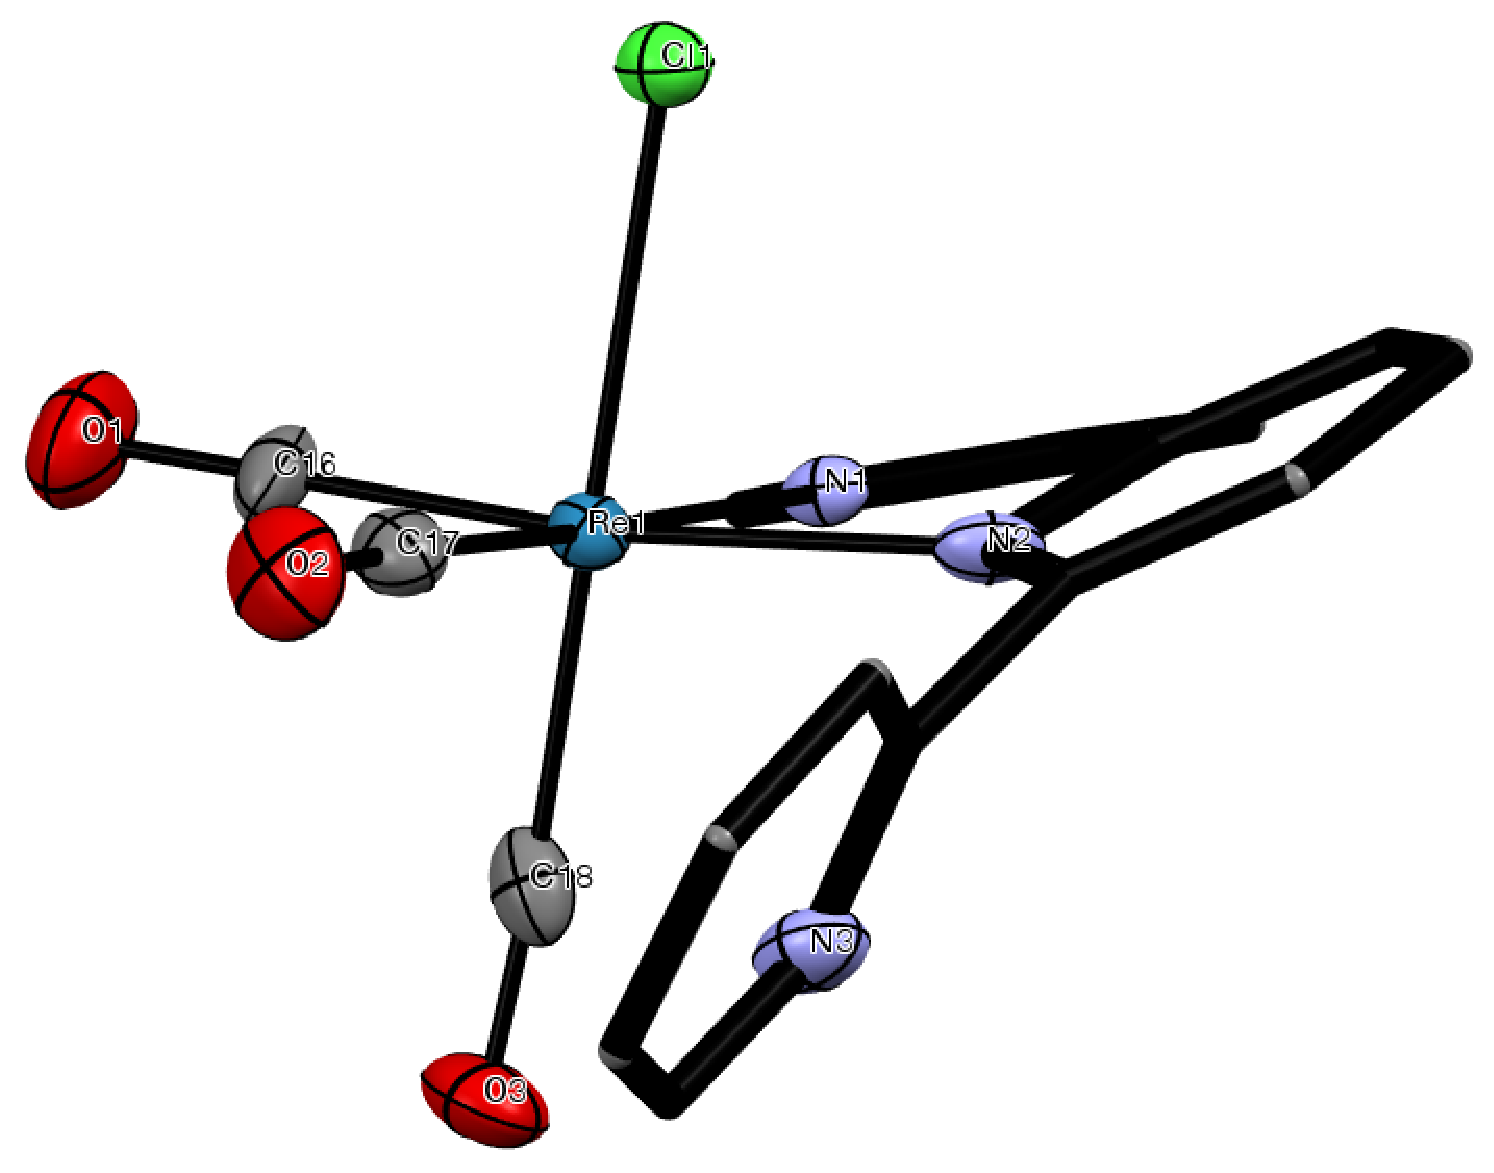
\includegraphics[clip=true, width=\textwidth, height=50mm, keepaspectratio]{images/xray1b.eps}
 \end{subfigure}
 \begin{subfigure}[b]{0.49\textwidth}
  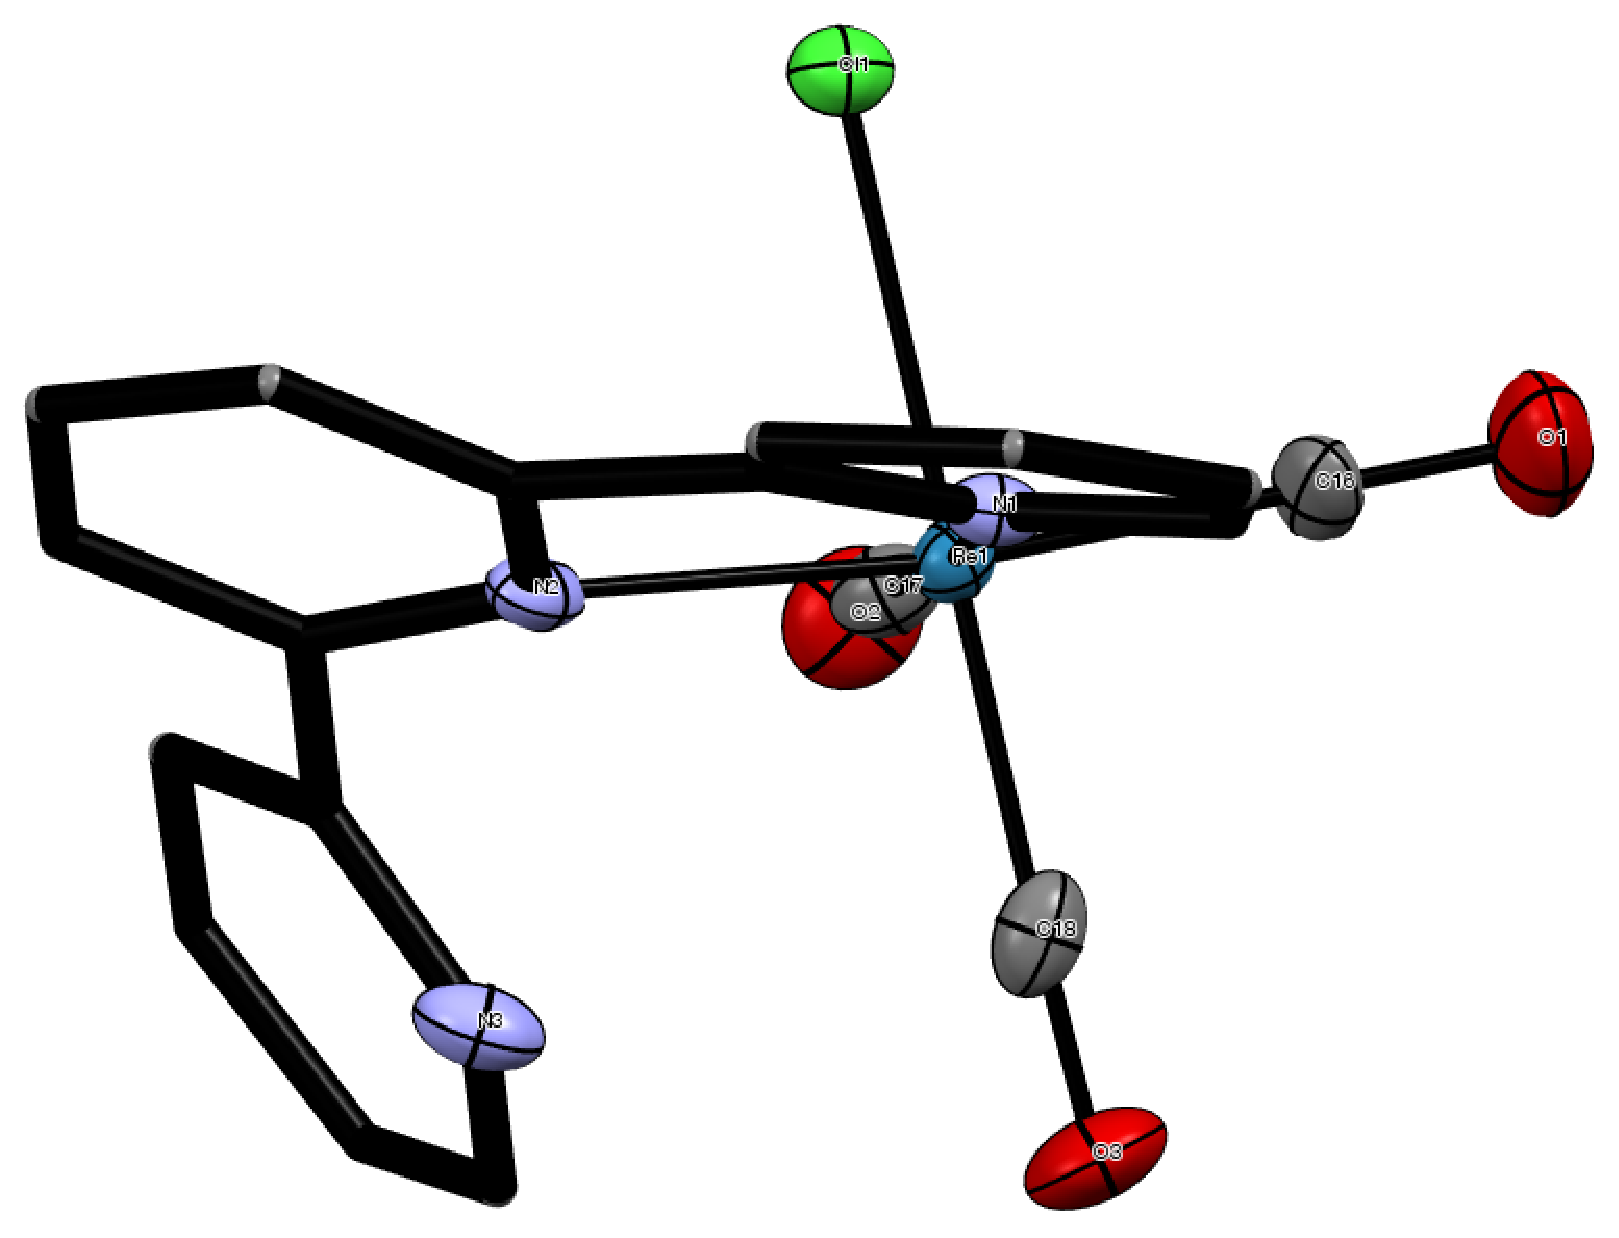
\includegraphics[clip=true, width=\textwidth, height=50mm, keepaspectratio]{images/xray1c.eps}
 \end{subfigure}
  \begin{subfigure}[b]{0.49\textwidth}
  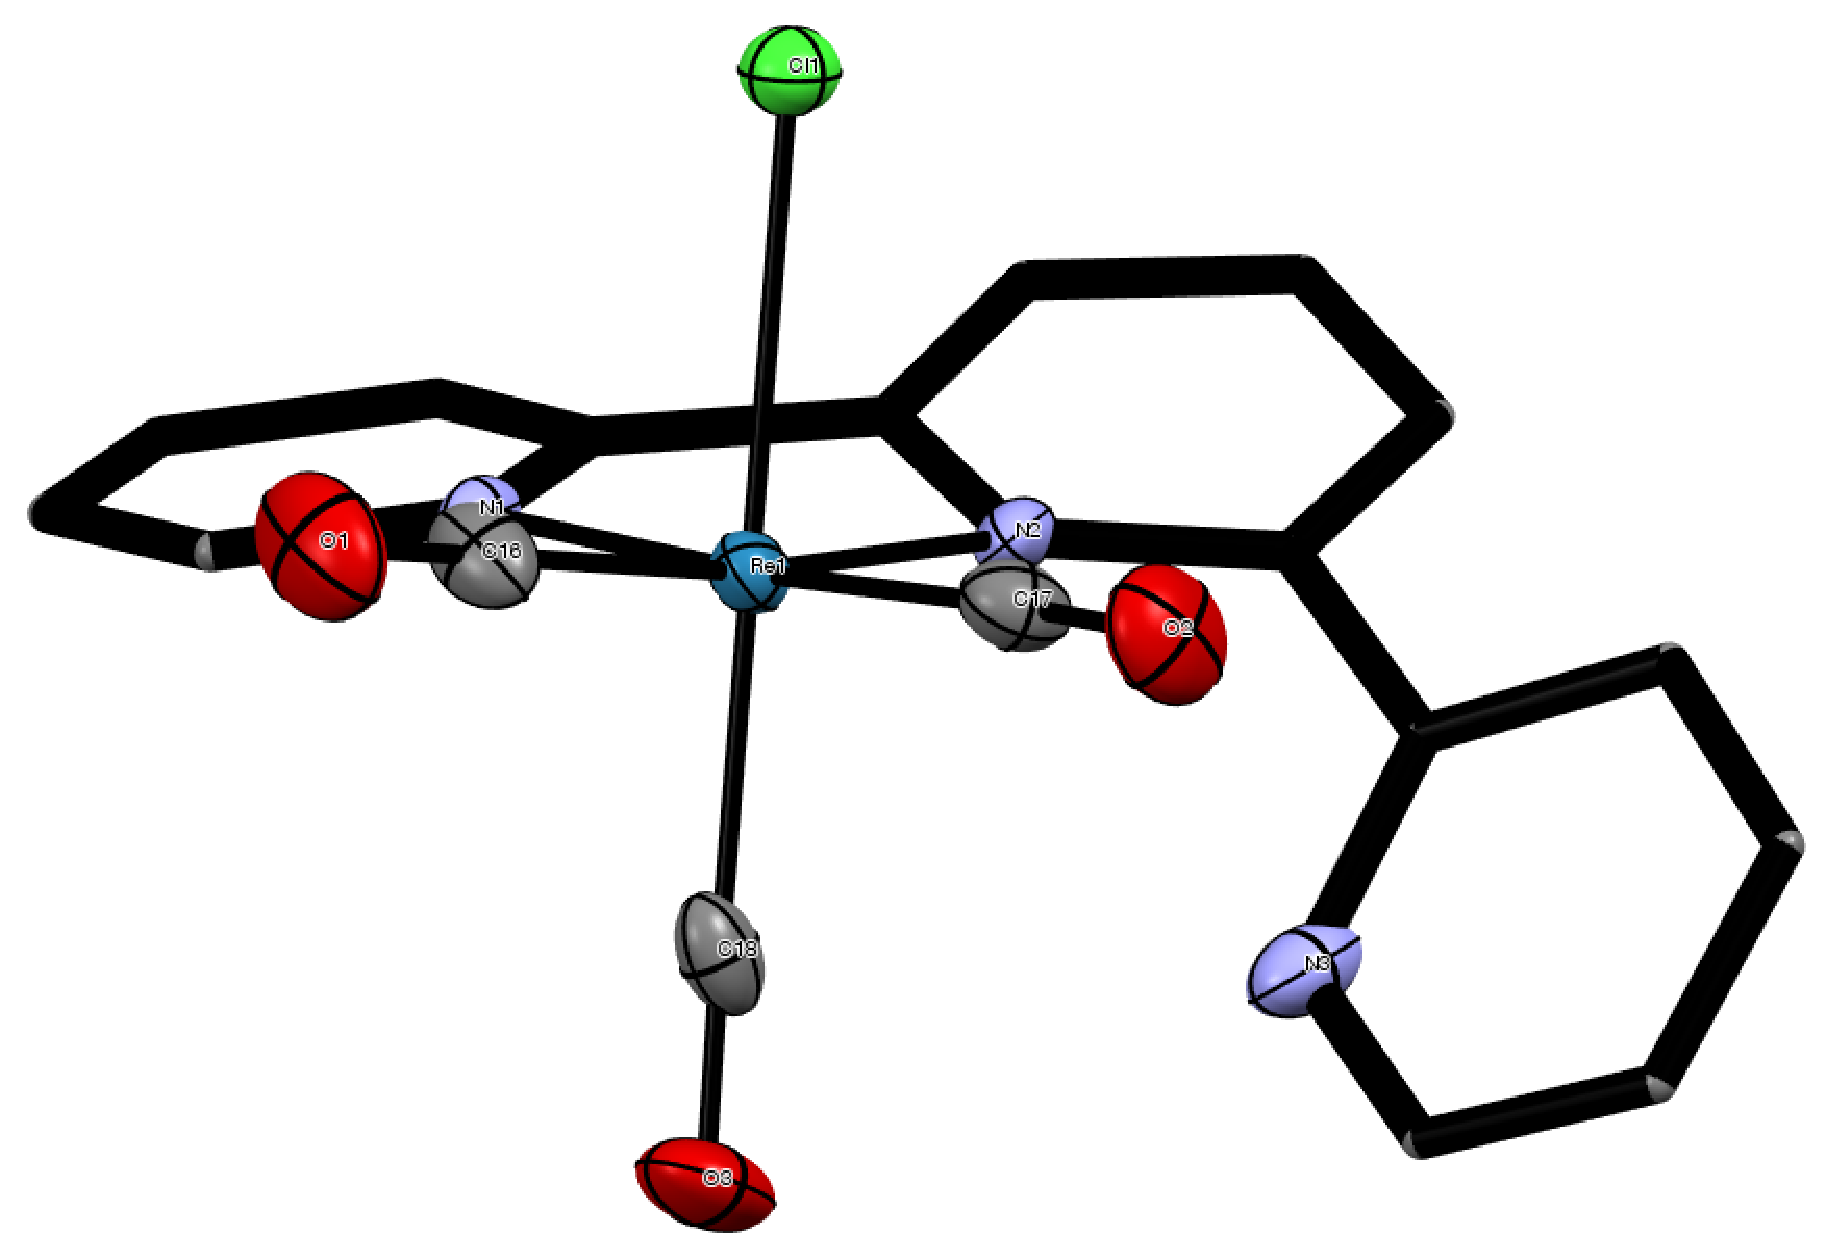
\includegraphics[clip=true, width=\textwidth, height=50mm, keepaspectratio]{images/xray1d.eps}
 \end{subfigure}
 \begin{subfigure}[b]{\textwidth}
  \centering
  \includegraphics[clip=true, width=\textwidth, height=75mm, keepaspectratio]{images/xray1uc.eps}
  \caption{Full unit cell representation of \textbf{2.1}}
 \end{subfigure}
\caption[X-ray crystal structure of \textbf{2.1}]{X-ray crystal structure of \textbf{2.1}. Co-crystallized chloroform, hydrogen atoms, and thermal ellipsoids of ligand carbon atoms are omitted for clarity.}
\label{fig.xray21}
\end{figure}

\begin{figure}[!ht]
 \centering
 \begin{subfigure}[b]{0.49\textwidth}
  \includegraphics[clip=true, width=\textwidth, height=50mm, keepaspectratio]{images/xray2a.eps}
 \end{subfigure}
 \begin{subfigure}[b]{0.49\textwidth}
  \includegraphics[clip=true, width=\textwidth, height=50mm, keepaspectratio]{images/xray2b.eps}
 \end{subfigure}
 \begin{subfigure}[b]{0.49\textwidth}
  \includegraphics[clip=true, width=\textwidth, height=50mm, keepaspectratio]{images/xray2c.eps}
 \end{subfigure}
 \begin{subfigure}[b]{\textwidth}
  \centering
  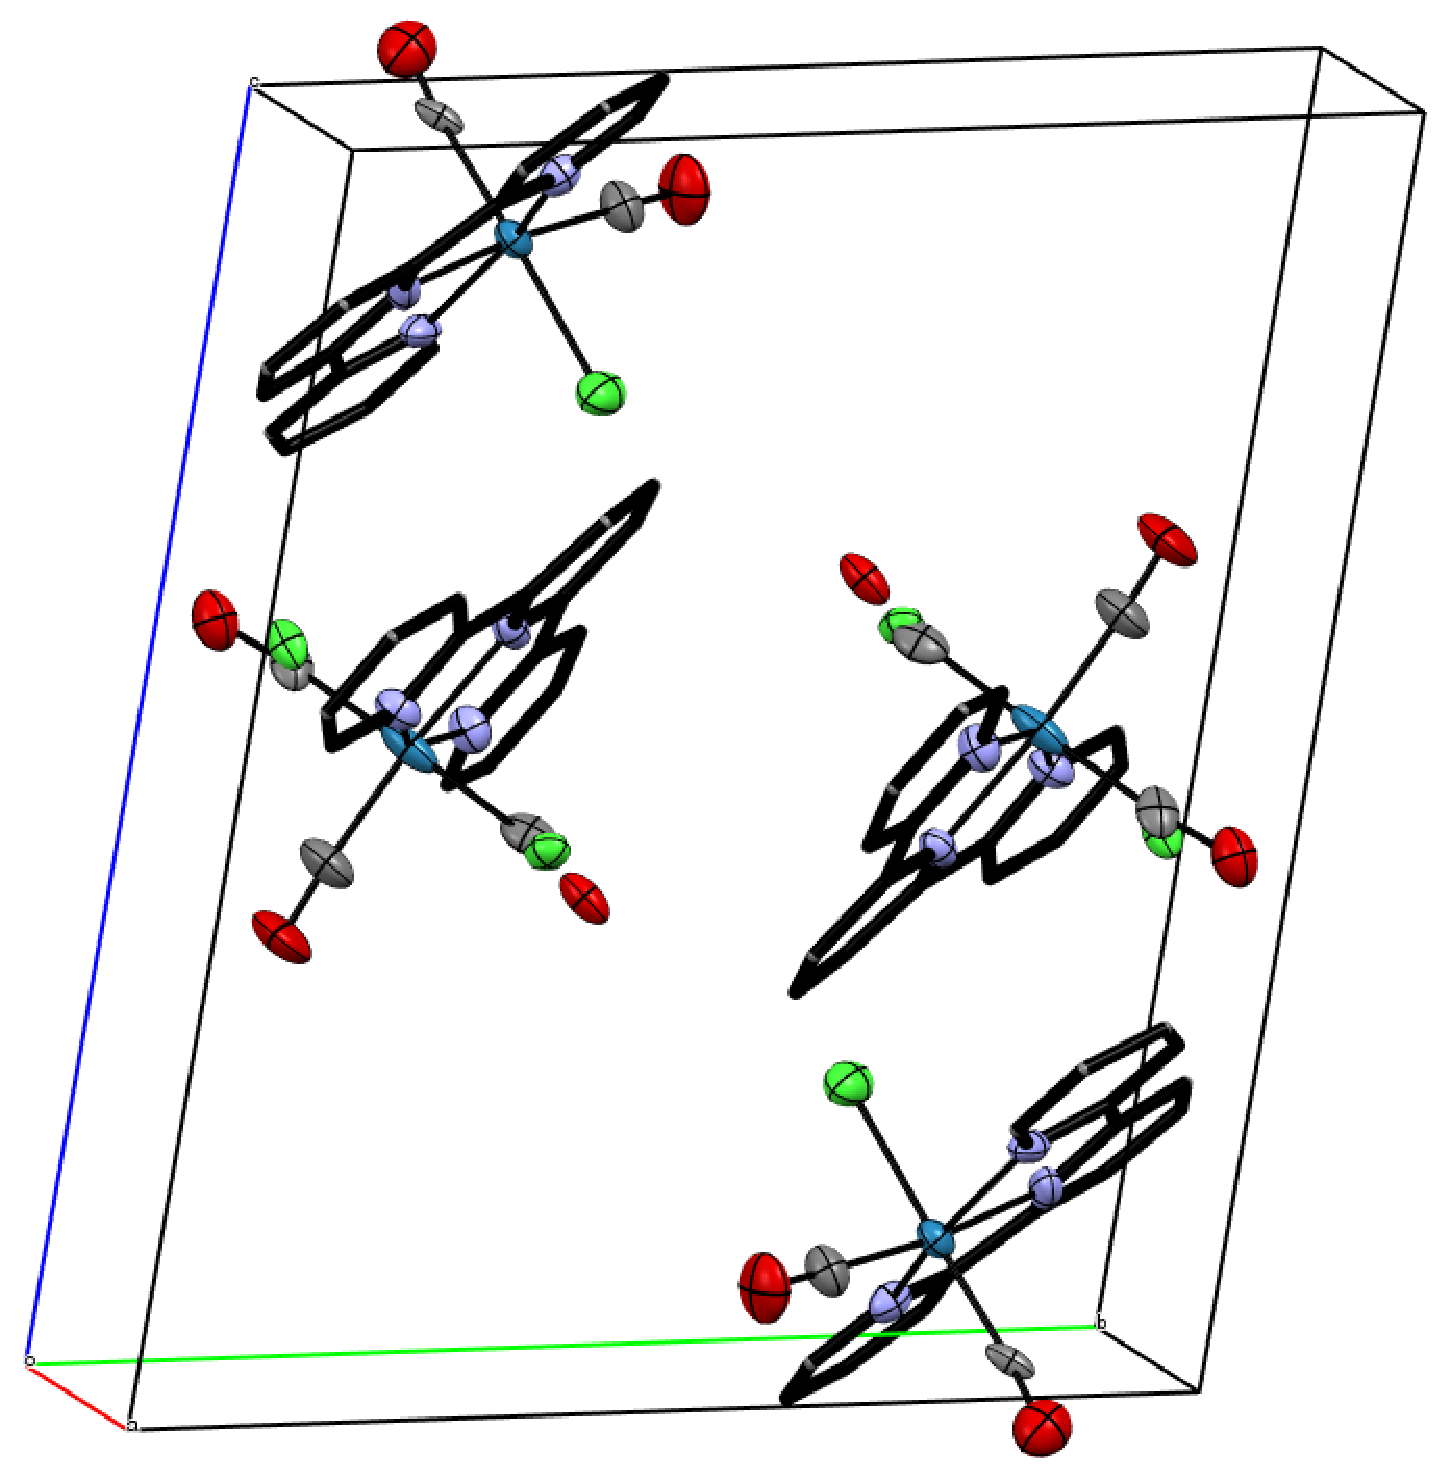
\includegraphics[clip=true, width=\textwidth, height=75mm, keepaspectratio]{images/xray2uc.eps}
  \caption{Full unit cell representation of \textbf{2.2}}
 \end{subfigure}
\caption[X-ray crystal structure of \textbf{2.2}]{X-ray crystal structure of \textbf{2.2}. Co-crystallized chloroform, hydrogen atoms, and thermal ellipsoids of ligand carbon atoms are omitted for clarity.}
\label{fig.xray22}
\end{figure}

\begin{figure}[!ht]
 \centering
 \begin{subfigure}[b]{0.49\textwidth}
  \includegraphics[clip=true, width=\textwidth, height=50mm, keepaspectratio]{images/xray3a.eps}
 \end{subfigure}
 \begin{subfigure}[b]{0.49\textwidth}
  \includegraphics[clip=true, width=\textwidth, height=50mm, keepaspectratio]{images/xray3b.eps}
 \end{subfigure}
 \begin{subfigure}[b]{0.49\textwidth}
  \includegraphics[clip=true, width=\textwidth, height=50mm, keepaspectratio]{images/xray3c.eps}
 \end{subfigure}
 \begin{subfigure}[b]{0.49\textwidth}
  \includegraphics[clip=true, width=\textwidth, height=50mm, keepaspectratio]{images/xray3d.eps}
 \end{subfigure}
 \begin{subfigure}[b]{\textwidth}
  \centering
  \includegraphics[clip=true, width=\textwidth, height=75mm, keepaspectratio]{images/xray3uc.eps}
  \caption{Full unit cell representation of \textbf{2.3}}
 \end{subfigure}
\caption[X-ray crystal structure of \textbf{2.3}]{X-ray crystal structure of \textbf{2.3}. Hydrogen atoms, and thermal ellipsoids of ligand carbon atoms are omitted for clarity.}
\label{fig.xray23}
\end{figure}

\begin{figure}[!ht]
 \centering
 \begin{subfigure}[b]{0.49\textwidth}
  \includegraphics[clip=true, width=\textwidth, height=50mm, keepaspectratio]{images/xray5a.eps}
 \end{subfigure}
 \begin{subfigure}[b]{0.49\textwidth}
  \includegraphics[clip=true, width=\textwidth, height=50mm, keepaspectratio]{images/xray5b.eps}
 \end{subfigure}
 \begin{subfigure}[b]{0.49\textwidth}
  \includegraphics[clip=true, width=\textwidth, height=50mm, keepaspectratio]{images/xray5c.eps}
 \end{subfigure}
 \begin{subfigure}[b]{0.49\textwidth}
  \includegraphics[clip=true, width=\textwidth, height=50mm, keepaspectratio]{images/xray5d.eps}
 \end{subfigure}
 \begin{subfigure}[b]{\textwidth}
  \centering
  \includegraphics[clip=true, width=\textwidth, height=75mm, keepaspectratio]{images/xray5uc.eps}
  \caption{Full unit cell representation of \textbf{2.5}}
 \end{subfigure}
\caption[X-ray crystal structure of \textbf{2.5}]{X-ray crystal structure of \textbf{2.5}. Hydrogen atoms, and thermal ellipsoids of ligand carbon atoms are omitted for clarity.}
\label{fig.xray25}
\end{figure}

\begin{figure}[!ht]
 \centering
 \begin{subfigure}[b]{0.49\textwidth}
  \includegraphics[clip=true, width=\textwidth, height=50mm, keepaspectratio]{images/xray8a.eps}
 \end{subfigure}
 \begin{subfigure}[b]{0.49\textwidth}
  \includegraphics[clip=true, width=\textwidth, height=50mm, keepaspectratio]{images/xray8b.eps}
 \end{subfigure}
 \begin{subfigure}[b]{0.49\textwidth}
  \includegraphics[clip=true, width=\textwidth, height=50mm, keepaspectratio]{images/xray8c.eps}
 \end{subfigure}
 \begin{subfigure}[b]{0.49\textwidth}
  \includegraphics[clip=true, width=\textwidth, height=50mm, keepaspectratio]{images/xray8d.eps}
 \end{subfigure}
 \begin{subfigure}[b]{\textwidth}
  \centering
  \includegraphics[clip=true, width=\textwidth, height=75mm, keepaspectratio]{images/xray8uc.eps}
  \caption{Full unit cell representation of \textbf{2.8}}
 \end{subfigure}
\caption[X-ray crystal structure of \textbf{2.8}]{X-ray crystal structure of \textbf{2.8}. Hydrogen atoms, and thermal ellipsoids of ligand carbon atoms are omitted for clarity.}
\label{fig.xray28}
\end{figure}
\cleardoublepage
% An appendix
%======================================================================
\chapter{Molecular Orbitals Diagrams} \label{app.mos}
\markright{Molecular Orbitals Diagrams}
%======================================================================

Frontier \glspl{ac.mo} for each compound discussed in this thesis are listed below in \Cref{fig.mo21,fig.mo22,fig.mo23,fig.mo24,fig.mo25,fig.mo26,fig.mo27,fig.mo28}. These orbitals are generated with the Chemissian program\autocite{chemissian}.

\begin{figure}[!ht]
 \centering
 \begin{subfigure}[b]{0.31\textwidth}
  \includegraphics[clip=true, width=\textwidth, keepaspectratio]{images/mos/1l+2.eps}
  \caption{LUMO+2}
 \end{subfigure}
  \begin{subfigure}[b]{0.31\textwidth}
  \includegraphics[clip=true, width=\textwidth, keepaspectratio]{images/mos/1l+1.eps}
  \caption{LUMO+1}
 \end{subfigure}
  \begin{subfigure}[b]{0.31\textwidth}
  \includegraphics[clip=true, width=\textwidth, keepaspectratio]{images/mos/1l.eps}
  \caption{LUMO}
 \end{subfigure}
 \begin{subfigure}[b]{0.31\textwidth}
  \includegraphics[clip=true, width=\textwidth, keepaspectratio]{images/mos/1h.eps}
  \caption{HOMO}
 \end{subfigure}
 \begin{subfigure}[b]{0.31\textwidth}
  \includegraphics[clip=true, width=\textwidth, keepaspectratio]{images/mos/1h-1.eps}
  \caption{HOMO-1}
 \end{subfigure}
 \begin{subfigure}[b]{0.31\textwidth}
  \includegraphics[clip=true, width=\textwidth, keepaspectratio]{images/mos/1h-2.eps}
  \caption{HOMO-2}
 \end{subfigure}
 \begin{subfigure}[b]{0.31\textwidth}
  \includegraphics[clip=true, width=\textwidth, keepaspectratio]{images/mos/1h-3.eps}
  \caption{HOMO-3}
 \end{subfigure}
\caption[Molecular orbitals HOMO-3 to LUMO+2 of \textbf{2.1}]{Isosurface plots of the frontier molecular orbitals HOMO-3 to LUMO+2 of \textbf{2.1}}
\label{fig.mo21}
\end{figure} 

\begin{figure}[!ht]
 \centering
 \begin{subfigure}[b]{0.31\textwidth}
  \includegraphics[clip=true, width=\textwidth, keepaspectratio]{images/mos/2l+3.eps}
  \caption{LUMO+3}
 \end{subfigure}
 \begin{subfigure}[b]{0.31\textwidth}
  \includegraphics[clip=true, width=\textwidth, keepaspectratio]{images/mos/2l+2.eps}
  \caption{LUMO+2}
 \end{subfigure}
  \begin{subfigure}[b]{0.31\textwidth}
  \includegraphics[clip=true, width=\textwidth, keepaspectratio]{images/mos/2l+1.eps}
  \caption{LUMO+1}
 \end{subfigure}
  \begin{subfigure}[b]{0.31\textwidth}
  \includegraphics[clip=true, width=\textwidth, keepaspectratio]{images/mos/2l.eps}
  \caption{LUMO}
 \end{subfigure}
 \begin{subfigure}[b]{0.31\textwidth}
  \includegraphics[clip=true, width=\textwidth, keepaspectratio]{images/mos/2h.eps}
  \caption{HOMO}
 \end{subfigure}
 \begin{subfigure}[b]{0.31\textwidth}
  \includegraphics[clip=true, width=\textwidth, keepaspectratio]{images/mos/2h-1.eps}
  \caption{HOMO-1}
 \end{subfigure}
 \begin{subfigure}[b]{0.31\textwidth}
  \includegraphics[clip=true, width=\textwidth, keepaspectratio]{images/mos/2h-2.eps}
  \caption{HOMO-2}
 \end{subfigure}
 \begin{subfigure}[b]{0.31\textwidth}
  \includegraphics[clip=true, width=\textwidth, keepaspectratio]{images/mos/2h-3.eps}
  \caption{HOMO-3}
 \end{subfigure}
 \begin{subfigure}[b]{0.31\textwidth}
  \includegraphics[clip=true, width=\textwidth, keepaspectratio]{images/mos/2h-4.eps}
  \caption{HOMO-5}
 \end{subfigure}
 \begin{subfigure}[b]{0.31\textwidth}
  \includegraphics[clip=true, width=\textwidth, keepaspectratio]{images/mos/2h-5.eps}
  \caption{HOMO-5}
 \end{subfigure}
\caption[Molecular orbitals HOMO-5 to LUMO+3 of \textbf{2.2}]{Isosurface plots of the frontier molecular orbitals HOMO-5 to LUMO+3 of \textbf{2.2}}
\label{fig.mo22}
\end{figure} 

\begin{figure}[!ht]
 \centering
 \begin{subfigure}[b]{0.31\textwidth}
  \includegraphics[clip=true, width=\textwidth, keepaspectratio]{images/mos/3l+2.eps}
  \caption{LUMO+2}
 \end{subfigure}
  \begin{subfigure}[b]{0.31\textwidth}
  \includegraphics[clip=true, width=\textwidth, keepaspectratio]{images/mos/3l+1.eps}
  \caption{LUMO+1}
 \end{subfigure}
  \begin{subfigure}[b]{0.31\textwidth}
  \includegraphics[clip=true, width=\textwidth, keepaspectratio]{images/mos/3l.eps}
  \caption{LUMO}
 \end{subfigure}
 \begin{subfigure}[b]{0.31\textwidth}
  \includegraphics[clip=true, width=\textwidth, keepaspectratio]{images/mos/3h.eps}
  \caption{HOMO}
 \end{subfigure}
 \begin{subfigure}[b]{0.31\textwidth}
  \includegraphics[clip=true, width=\textwidth, keepaspectratio]{images/mos/3h-1.eps}
  \caption{HOMO-1}
 \end{subfigure}
 \begin{subfigure}[b]{0.31\textwidth}
  \includegraphics[clip=true, width=\textwidth, keepaspectratio]{images/mos/3h-2.eps}
  \caption{HOMO-2}
 \end{subfigure}
 \begin{subfigure}[b]{0.31\textwidth}
  \includegraphics[clip=true, width=\textwidth, keepaspectratio]{images/mos/3h-3.eps}
  \caption{HOMO-3}
 \end{subfigure}
\caption[Molecular orbitals HOMO-3 to LUMO+2 of \textbf{2.3}]{Isosurface plots of the frontier molecular orbitals HOMO-3 to LUMO+2 of \textbf{2.3}}
\label{fig.mo23}
\end{figure} 

\begin{figure}[!ht]
 \centering
 \begin{subfigure}[b]{0.31\textwidth}
  \includegraphics[clip=true, width=\textwidth, keepaspectratio]{images/mos/4l+3.eps}
  \caption{LUMO+3}
 \end{subfigure}
 \begin{subfigure}[b]{0.31\textwidth}
  \includegraphics[clip=true, width=\textwidth, keepaspectratio]{images/mos/4l+2.eps}
  \caption{LUMO+2}
 \end{subfigure}
  \begin{subfigure}[b]{0.31\textwidth}
  \includegraphics[clip=true, width=\textwidth, keepaspectratio]{images/mos/4l+1.eps}
  \caption{LUMO+1}
 \end{subfigure}
  \begin{subfigure}[b]{0.31\textwidth}
  \includegraphics[clip=true, width=\textwidth, keepaspectratio]{images/mos/4l.eps}
  \caption{LUMO}
 \end{subfigure}
 \begin{subfigure}[b]{0.31\textwidth}
  \includegraphics[clip=true, width=\textwidth, keepaspectratio]{images/mos/4h.eps}
  \caption{HOMO}
 \end{subfigure}
 \begin{subfigure}[b]{0.31\textwidth}
  \includegraphics[clip=true, width=\textwidth, keepaspectratio]{images/mos/4h-1.eps}
  \caption{HOMO-1}
 \end{subfigure}
 \begin{subfigure}[b]{0.31\textwidth}
  \includegraphics[clip=true, width=\textwidth, keepaspectratio]{images/mos/4h-2.eps}
  \caption{HOMO-2}
 \end{subfigure}
 \begin{subfigure}[b]{0.31\textwidth}
  \includegraphics[clip=true, width=\textwidth, keepaspectratio]{images/mos/4h-3.eps}
  \caption{HOMO-3}
 \end{subfigure}
 \begin{subfigure}[b]{0.31\textwidth}
  \includegraphics[clip=true, width=\textwidth, keepaspectratio]{images/mos/4h-4.eps}
  \caption{HOMO-5}
 \end{subfigure}
 \begin{subfigure}[b]{0.31\textwidth}
  \includegraphics[clip=true, width=\textwidth, keepaspectratio]{images/mos/4h-5.eps}
  \caption{HOMO-5}
 \end{subfigure}
\caption[Molecular orbitals HOMO-5 to LUMO+3 of \textbf{2.4}]{Isosurface plots of the frontier molecular orbitals HOMO-5 to LUMO+3 of \textbf{2.4}}
\label{fig.mo24}
\end{figure}

\begin{figure}[!ht]
 \centering
 \begin{subfigure}[b]{0.31\textwidth}
  \includegraphics[clip=true, width=\textwidth, keepaspectratio]{images/mos/5l+2.eps}
  \caption{LUMO+2}
 \end{subfigure}
  \begin{subfigure}[b]{0.31\textwidth}
  \includegraphics[clip=true, width=\textwidth, keepaspectratio]{images/mos/5l+1.eps}
  \caption{LUMO+1}
 \end{subfigure}
  \begin{subfigure}[b]{0.31\textwidth}
  \includegraphics[clip=true, width=\textwidth, keepaspectratio]{images/mos/5l.eps}
  \caption{LUMO}
 \end{subfigure}
 \begin{subfigure}[b]{0.31\textwidth}
  \includegraphics[clip=true, width=\textwidth, keepaspectratio]{images/mos/5h.eps}
  \caption{HOMO}
 \end{subfigure}
 \begin{subfigure}[b]{0.31\textwidth}
  \includegraphics[clip=true, width=\textwidth, keepaspectratio]{images/mos/5h-1.eps}
  \caption{HOMO-1}
 \end{subfigure}
 \begin{subfigure}[b]{0.31\textwidth}
  \includegraphics[clip=true, width=\textwidth, keepaspectratio]{images/mos/5h-2.eps}
  \caption{HOMO-2}
 \end{subfigure}
 \begin{subfigure}[b]{0.31\textwidth}
  \includegraphics[clip=true, width=\textwidth, keepaspectratio]{images/mos/5h-3.eps}
  \caption{HOMO-3}
 \end{subfigure}
\caption[Molecular orbitals HOMO-3 to LUMO+2 of \textbf{2.5}]{Isosurface plots of the frontier molecular orbitals HOMO-3 to LUMO+2 of \textbf{2.5}}
\label{fig.mo25}
\end{figure} 

\begin{figure}[!ht]
 \centering
 \begin{subfigure}[b]{0.31\textwidth}
  \includegraphics[clip=true, width=\textwidth, keepaspectratio]{images/mos/6l+3.eps}
  \caption{LUMO+3}
 \end{subfigure}
 \begin{subfigure}[b]{0.31\textwidth}
  \includegraphics[clip=true, width=\textwidth, keepaspectratio]{images/mos/6l+2.eps}
  \caption{LUMO+2}
 \end{subfigure}
  \begin{subfigure}[b]{0.31\textwidth}
  \includegraphics[clip=true, width=\textwidth, keepaspectratio]{images/mos/6l+1.eps}
  \caption{LUMO+1}
 \end{subfigure}
  \begin{subfigure}[b]{0.31\textwidth}
  \includegraphics[clip=true, width=\textwidth, keepaspectratio]{images/mos/6l.eps}
  \caption{LUMO}
 \end{subfigure}
 \begin{subfigure}[b]{0.31\textwidth}
  \includegraphics[clip=true, width=\textwidth, keepaspectratio]{images/mos/6h.eps}
  \caption{HOMO}
 \end{subfigure}
 \begin{subfigure}[b]{0.31\textwidth}
  \includegraphics[clip=true, width=\textwidth, keepaspectratio]{images/mos/6h-1.eps}
  \caption{HOMO-1}
 \end{subfigure}
 \begin{subfigure}[b]{0.31\textwidth}
  \includegraphics[clip=true, width=\textwidth, keepaspectratio]{images/mos/6h-2.eps}
  \caption{HOMO-2}
 \end{subfigure}
 \begin{subfigure}[b]{0.31\textwidth}
  \includegraphics[clip=true, width=\textwidth, keepaspectratio]{images/mos/6h-3.eps}
  \caption{HOMO-3}
 \end{subfigure}
 \begin{subfigure}[b]{0.31\textwidth}
  \includegraphics[clip=true, width=\textwidth, keepaspectratio]{images/mos/6h-4.eps}
  \caption{HOMO-5}
 \end{subfigure}
 \begin{subfigure}[b]{0.31\textwidth}
  \includegraphics[clip=true, width=\textwidth, keepaspectratio]{images/mos/6h-5.eps}
  \caption{HOMO-5}
 \end{subfigure}
\caption[Molecular orbitals HOMO-5 to LUMO+3 of \textbf{2.6}]{Isosurface plots of the frontier molecular orbitals HOMO-5 to LUMO+3 of \textbf{2.6}}
\label{fig.mo26}
\end{figure}

\begin{figure}[!ht]
 \centering
 \begin{subfigure}[b]{0.31\textwidth}
  \includegraphics[clip=true, width=\textwidth, keepaspectratio]{images/mos/7l+2.eps}
  \caption{LUMO+2}
 \end{subfigure}
  \begin{subfigure}[b]{0.31\textwidth}
  \includegraphics[clip=true, width=\textwidth, keepaspectratio]{images/mos/7l+1.eps}
  \caption{LUMO+1}
 \end{subfigure}
  \begin{subfigure}[b]{0.31\textwidth}
  \includegraphics[clip=true, width=\textwidth, keepaspectratio]{images/mos/7l.eps}
  \caption{LUMO}
 \end{subfigure}
 \begin{subfigure}[b]{0.31\textwidth}
  \includegraphics[clip=true, width=\textwidth, keepaspectratio]{images/mos/7h.eps}
  \caption{HOMO}
 \end{subfigure}
 \begin{subfigure}[b]{0.31\textwidth}
  \includegraphics[clip=true, width=\textwidth, keepaspectratio]{images/mos/7h-1.eps}
  \caption{HOMO-1}
 \end{subfigure}
 \begin{subfigure}[b]{0.31\textwidth}
  \includegraphics[clip=true, width=\textwidth, keepaspectratio]{images/mos/7h-2.eps}
  \caption{HOMO-2}
 \end{subfigure}
 \begin{subfigure}[b]{0.31\textwidth}
  \includegraphics[clip=true, width=\textwidth, keepaspectratio]{images/mos/7h-3.eps}
  \caption{HOMO-3}
 \end{subfigure}
\caption[Molecular orbitals HOMO-3 to LUMO+2 of \textbf{2.7}]{Isosurface plots of the frontier molecular orbitals HOMO-3 to LUMO+2 of \textbf{2.7}}
\label{fig.mo27}
\end{figure} 

\begin{figure}[!ht]
 \centering
 \begin{subfigure}[b]{0.31\textwidth}
  \includegraphics[clip=true, width=\textwidth, keepaspectratio]{images/mos/8l+3.eps}
  \caption{LUMO+3}
 \end{subfigure}
 \begin{subfigure}[b]{0.31\textwidth}
  \includegraphics[clip=true, width=\textwidth, keepaspectratio]{images/mos/8l+2.eps}
  \caption{LUMO+2}
 \end{subfigure}
  \begin{subfigure}[b]{0.31\textwidth}
  \includegraphics[clip=true, width=\textwidth, keepaspectratio]{images/mos/8l+1.eps}
  \caption{LUMO+1}
 \end{subfigure}
  \begin{subfigure}[b]{0.31\textwidth}
  \includegraphics[clip=true, width=\textwidth, keepaspectratio]{images/mos/8l.eps}
  \caption{LUMO}
 \end{subfigure}
 \begin{subfigure}[b]{0.31\textwidth}
  \includegraphics[clip=true, width=\textwidth, keepaspectratio]{images/mos/8h.eps}
  \caption{HOMO}
 \end{subfigure}
 \begin{subfigure}[b]{0.31\textwidth}
  \includegraphics[clip=true, width=\textwidth, keepaspectratio]{images/mos/8h-1.eps}
  \caption{HOMO-1}
 \end{subfigure}
 \begin{subfigure}[b]{0.31\textwidth}
  \includegraphics[clip=true, width=\textwidth, keepaspectratio]{images/mos/8h-2.eps}
  \caption{HOMO-2}
 \end{subfigure}
 \begin{subfigure}[b]{0.31\textwidth}
  \includegraphics[clip=true, width=\textwidth, keepaspectratio]{images/mos/8h-3.eps}
  \caption{HOMO-3}
 \end{subfigure}
 \begin{subfigure}[b]{0.31\textwidth}
  \includegraphics[clip=true, width=\textwidth, keepaspectratio]{images/mos/8h-4.eps}
  \caption{HOMO-5}
 \end{subfigure}
 \begin{subfigure}[b]{0.31\textwidth}
  \includegraphics[clip=true, width=\textwidth, keepaspectratio]{images/mos/8h-5.eps}
  \caption{HOMO-5}
 \end{subfigure}
\caption[Molecular orbitals HOMO-5 to LUMO+3 of \textbf{2.8}]{Isosurface plots of the frontier molecular orbitals HOMO-5 to LUMO+3 of \textbf{2.8}}
\label{fig.mo28}
\end{figure}

\cleardoublepage
% An appendix
%======================================================================
\chapter{Reaction Potential Energy Diagrams} \label{app.energy}
\markright{Reaction Potential Energy Diagrams}
%======================================================================

Potential energy diagrams for the reactions discussed in \autoref{chap.mech} are listed below in \Cref{fig.pes_all,fig.pes_axial,fig.pes_planar,fig.pes_formate,fig.pes_wgs,fig.pes_carbonate,fig.pes_gas,fig.pes_dmf,fig.pes_eximer}. 

\begin{landscape}

\begin{figure}[!htbp]
 \begin{center}
  \includegraphics[clip=true, height=144mm, keepaspectratio]{images/pes_all.eps}
 \end{center}
\caption{An overview of the energies of the three mechanistic pathways of photochemical \ce{CO2} reduction}
\label{fig.pes_all}

\end{figure} 
\begin{figure}[!htbp]
 \begin{center}
  \includegraphics[clip=true, height=144mm, keepaspectratio]{images/pes_axial.eps}
 \end{center}
\caption{Potential Energy Surface for the axial geometry of the water-gas shift mechanistic pathway}
\label{fig.pes_axial}

\end{figure} 
\begin{figure}[!htbp]
 \begin{center}
  \includegraphics[clip=true, height=144mm, keepaspectratio]{images/pes_planar.eps}
 \end{center}
\caption{Potential Energy Surface for the planar geometry of the water-gas shift mechanistic pathway}
\label{fig.pes_planar}

\end{figure} 
\begin{figure}[!htbp]
 \begin{center}
  \includegraphics[clip=true, height=144mm, keepaspectratio]{images/pes_wgs.eps}
 \end{center}
\caption{Potential Energy Surface for the two water-gas shift mechanistic pathway geometries}
\label{fig.pes_wgs}
\end{figure} 

\begin{figure}[!htbp]
 \begin{center}
  \includegraphics[clip=true, height=144mm, keepaspectratio]{images/pes_formate.eps}
 \end{center}
\caption{Potential Energy Surface for the formate mechanistic pathway}
\label{fig.pes_formate}

\end{figure} 
\begin{figure}[!htbp]
 \begin{center}
  \includegraphics[clip=true, height=144mm, keepaspectratio]{images/pes_carbonate.eps}
 \end{center}
\caption{Potential Energy Surface for the carbonate mechanistic pathway}
\label{fig.pes_carbonate}

\end{figure} 
\begin{figure}[!htbp]
 \begin{center}
  \includegraphics[clip=true, height=144mm, keepaspectratio]{images/pes_gas.eps}
 \end{center}
\caption{An overview of the energies of the three mechanistic pathways of photochemical \ce{CO2} reduction in gas phase}
\label{fig.pes_gas}
\end{figure} 

\begin{figure}[!htbp]
 \begin{center}
  \includegraphics[clip=true, height=144mm, keepaspectratio]{images/pes_dmf.eps}
 \end{center}
\caption{An overview of the energies of the three mechanistic pathways of photochemical \ce{CO2} reduction in DMF}
\label{fig.pes_dmf}
\end{figure} 

\begin{figure}[!htbp]
 \begin{center}
  \includegraphics[clip=true, height=144mm, keepaspectratio]{images/pes_eximer.eps}
 \end{center}
\caption{Potential Energy Surface for the production of the eximer}
\label{fig.pes_eximer}
\end{figure} 

\end{landscape}
\cleardoublepage
\chapter{TurboControl and TurboGo Manual}\label{chap.readme}
\markright{TurboControl User's Manual}


TurboControl is a series of scripts to run Turbomole jobs from Gaussian style inputs. The following is the user manual included with distributions of TurboControl 

\section{Introduction}
Gaussian software is well known for the user friendly GUI it contains
(via GaussView). Turbomole, another computational suite, is known for
its speed and optimizations, but has a significantly higher learning
curve and is less beginner friendly. This software is an attempt to be
able to use the user friendly input from Gaussian to smooth over the use
of Turbomole.

\section{System Requirements}

There are two user-facing scripts available, both written to work with
Turbomole 6.1-6.5 on clusters using Grid Engine queuing software. The
only tests of operation are on a system with the following details:

\begin{itemize}
\itemsep1pt\parskip0pt\parsep0pt
\item
  Rocks 6.1 (Emerald Boa)/CentOS 6.3
\item
  Open Grid Scheduler/Grid Engine 2011.11p1
\item
  Python 2.7.3
\end{itemize}

Other systems, including different operating systems, different versions
of Grid Engine or python, or on other systems, are not supported.

Python dependencies include:

\begin{itemize}
\itemsep1pt\parskip0pt\parsep0pt
\item
  pexpect 3.2\autocite{pexpect}
\item
  openbabel\autocite{openbabel, oboyle2011} (optional)
\end{itemize}

Prior to running TurboGo or TurboControl, a valid installation of
Turbomole must be available. On systems where computational modules must
be loaded, Turbomole must have been loaded to the environment.
Additionally, running the Turbomole environment configuration is
recommended but not required prior to launching TurboGo or TurboControl:

\begin{center}
\begin{verbatim}
$ source $TURBODIR/Config_turbo_env
\end{verbatim}
\end{center}

\section{TurboGo}

TurboGo is a script fun on an input file. It generates the inputs
required for Turbomole jobs, and submits the job to the GridEngine queue
before quitting. TurboGo is run with the following syntax:

\begin{center}
\begin{verbatim}
$ turbogo [-h] [-v] [-q] file
\end{verbatim}
\end{center}

positional arguments:

\begin{Verbatim}[baselinestretch=0.75]
file                  Read input from gaussian-type input FILE.
\end{Verbatim}

More info on the input files is available below.

optional arguments:

\begin{itemize}
\item \texttt{-h, --help            }Show this help message and exit
\item \texttt{-v, --verbose         }Run more verbose (show debugging info)
\item \texttt{-q, --quiet           }Run less verbose (show only warnings)
\end{itemize}

TurboGo saves a log file (turbogo.log) in the directory in which it is
run. A second logfile (define.log) will remain if the setup crashes or
is terminated at some points, or if the script is run verbose.

TurboGo writes the final coordinates to final\_geometry.xyz. If
openbabel is installed, it will also write finalgeom.mol. The entire
optimization is written to optimization.xyz for viewing with a molecular
viewer, such as vmd.

\section{TurboControl}

TurboControl is a management script called from a parent directory
containing sub directories of input files. Each input file must be in
its own directory. The input file format must be the same as the input
format for TurboGo (listed above), with the extension `.in', `.inp',
`.input', `.com', or `.gjf'. TurboControl reads the inputs and submits
the jobs to the computational cluster queue. It then monitors running
jobs to determine when the script has finished. If the job is an
Opt-Freq, it prepares the frequency analysis and resubmits to the queue.
TurboControl analyzes completed Opt-Freq jobs for true optimization, and
attempts to re-run jobs with modified geometries when Transition States
are found. TurboControl will not get stuck on the same transition state,
but will return a `stuck' job. TurboControl is run with the following
syntax:

\begin{center}
\begin{verbatim}
$ turbocontrol [-h] [-v/-q] [-s]
\end{verbatim}
\end{center}

Optional arguments:

\begin{itemize}
\item \texttt{-h, --help            }Show this help message and exit
\item \texttt{-v, --verbose         }Run more verbose (show debugging info)
\item \texttt{-q, --quiet           }Run less verbose (show only warnings)
\item \texttt{-s, --solvent         }List available solvents for COSMO and quit
\end{itemize}

TurboControl outputs information every 3 hours on the status of the
jobs. It writes a logfile (\texttt{turbocontrol.log}) and may or may not leave
other log files in each directory (depending on verbosity level). Ends
when the last job finishes or crashes. Requires 1 node or can be run on
headnode (minimal resource consumption especially after initial job
preparation and submission.)

TurboControl assists with analysis by outputting a \texttt{stats.txt} file as jobs
complete. This file contains file details, optimization and frequency
timing details, energy, and the first frequency. Additional information
can be requested by including the \texttt{freeh} keyword (see below).

\section{Input File Format}

The input file format is similar to that well known by Gaussian users. A
series of keywords, one per line and indicated by a `\%', is followed by
the `route card' (specific job information). Charge and spin is
indicated, then the molecule is shown in Cartesian format. This is
followed by optional modifications to the Turbomole Control file. Note
the location of blank lines in the example (Section 5.7).

\subsection{Keywords}

Keywords are as follows:

\begin{itemize}
\item \texttt{\%nproc} - number of processors to use for the calculation job.
  \begin{itemize}
    \item Synonym: \texttt{\%nprocessors}
  \end{itemize}
\item \texttt{\%arch} - parallelization architecture to use for the job.
  \begin{itemize}
    \item Synonyms: \texttt{\%architecture}, \texttt{\%para\_arch}
   \end {itemize}
\item \texttt{\%maxcycles} - number of optimization iterations before failing.
\item \texttt{\%autocontrolmod} - DEFAULT - modify the \texttt{control} file to include optimizations to speed up the job.
\item \texttt{\%nocontrolmod} - do not modify \texttt{control} file as above.
\item \texttt{\%rt} - specify max expected runtime (for any part of job)in hours. Allows backfilling in gridengine queue to speed up job submission. For example, for a 1 hour opt and 4 hour freq, submit at least a \texttt{rt} of 4
\item \texttt{\%cosmo} - use turbomole's COSMO solvation model with the specificed solvent or \texttt{None} to use the idealized solvent (epsilon = infinity). List of available solvents can be shown by running \texttt{turbocontrol -s}
\end{itemize}

Gaussian args, including \texttt{\%nosave}, \texttt{\%rwf={[}file{]}}, \texttt{\%chk={[}file{]}}, and \texttt{\%mem={[}memory{]}} are silently ignored.

\subsection{Route Card Options}

Route cards take the form of the following:

\texttt{\# {[}jobtype(s){]} {[}joboption(s){]}}

Job types available:

\begin{itemize}
\item \texttt{opt} - Perform a geometry optimization
\item \texttt{freq} - Perform a frequency analysis. Specify method via numforce or aoforce. default = numforce
\item \texttt{sp} - Perform a single point energy calculation.
  \begin{itemize}
    \item Cannot be combined with Opt or Freq
  \end{itemize}
\item \texttt{ts} - Perform a transition state search to find 1 imaginary vibration. 
  \begin{itemize}
    \item Cannot be combined with Opt or Freq
  \end{itemize}
\item \texttt{prep} - Prepare the job but do not submit to queue.
  \begin{itemize}
    \item Cannot be combined with Opt or Freq
  \end{itemize}
\end{itemize}

Job options available:

\begin{itemize}
\item \texttt{ri} - Use Turbomole's ri approximation
\item \texttt{marij} - Use Turbomole's marij approximation 
  \begin{itemize}
    \item Requires \texttt{ri}
  \end{itemize}
\item \texttt{disp} - Use Turbomole's implementation of Grimme's dispersion, version 3
\item \texttt{aoforce} - Use aoforce for frequency jobs
\item \texttt{numforce} - Use numforce for frequency jobs
\item \texttt{freeh} - Use Turbomole's \texttt{freeh} thermodynamics data script to extract thermodynamic information after frequency analysis
\end{itemize}

\subsection{Title}

Following the Route cards, a blank line is added, then a line containing
the title of the calculation. This can include any characters, spaces,
etc., remaining on only one line. This is followed by a blank line.

\subsection{Charge and Spin}

Charge and spin are listed as two numbers separated by a space: charge spin (eg:0 1)

\subsection{Geometry}

Geometry in xyz coordinate format: Element xcoord ycoord zcoord. Z-matrix geometry is not supported by TurboControl or TurboGo.

\subsection{Additional control File Modifications}

Additional lines to be added or removed from control. Lines
automatically added are, as required,:

\begin{Verbatim}[baselinestretch=0.75]
$ricore 0
$paroptions ga_memperproc 900000000000000 900000000000
$parallel_parameters  maxtask=10000
$ricore_slave 1
$maxcor 2048
\end{Verbatim}

Additional lines may be added, or lines removed, by placing them after
the geometry with a \texttt{\$} (for addition) or \texttt{-\$} (for removal).

\subsection{Example Input File}

An example input file for benzene in dmf:

\begin{Verbatim}[baselinestretch=0.75]
%nproc=4
%arch=GA
%maxcycles=250
%rt=6
%cosmo=dmf
# opt freq b3-lyp/def2-TZVP ri marij numforce

Benzene Optimization & Frequency

0 1
C  0.000  1.396  0.000
C  1.209  0.698  0.000
C  1.209 -0.698  0.000
C  0.000 -1.396  0.000
C -1.209 -0.698  0.000
C -1.209  0.698  0.000
H  0.000  2.479  0.000
H  2.147  1.240  0.000
H  2.147 -1.240  0.000
H  0.000 -2.479  0.000
H -2.147 -1.240  0.000
H -2.147  1.240  0.000

$disp
-$paraoptions

\end{Verbatim}


\section{Code Details}

Coverage percentages of code unittests are listed in \autoref{tab.codetest}. Results are low for def\_op, screwer\_op, cosmo\_op, freeh\_op, turbocontrol, and turbogo because they contain many lines of interacting with GridEngine or TurboMole. Testing is performed via monitoring the status of the scripts as they run in real conditions.

The code style is graded by PyLint and results are shown in \autoref{tab.pylint}. PyLint describes coding style, adherence to guidelines, and readability. It does not describe code efficiency or usefulness.

\begin{table}[!H]
  \centering
    \caption{Test Coverage of scripts in Turbocontrol}
    \begin{tabular}{crrrr}
    \toprule
    Name  & Statements & Missing & Excluded & Coverage \\
    \midrule
    cosmo\_op & 106   & 70    & 1     & 34\% \\
    cosmo\_op\_test & 17    & 1     & 0     & 94\% \\
    def\_op & 302   & 226   & 1     & 25\% \\
    def\_op\_test & 20    & 1     & 0     & 95\% \\
    freeh\_op & 162   & 55    & 1     & 66\% \\
    freeh\_op\_test & 27    & 1     & 0     & 96\% \\
    screwer\_op & 71    & 25    & 1     & 65\% \\
    screwer\_op\_test & 11    & 1     & 0     & 91\% \\
    test\_all & 18    & 0     & 0     & 100\% \\
    turbocontrol & 537   & 319   & 0     & 41\% \\
    turbocontrol\_test & 245   & 24    & 0     & 90\% \\
    turbogo & 343   & 132   & 0     & 62\% \\
    turbogo\_helpers & 383   & 52    & 0     & 86\% \\
    turbogo\_helpers\_test & 274   & 2     & 0     & 99\% \\
    turbogo\_test & 98    & 1     & 0     & 99\% \\
          & 2614  & 910   & 4     & 65\% \\
    \bottomrule
    \end{tabular}%
  \label{tab.codetest}
\end{table}%

\begin{table}[!h]
  \centering
  \caption{PyLint Scores for Turbocontrol Code}
    \begin{tabular}{cr}
    \toprule
    File  & Score /10 \\
    \midrule
    test\_all.py & 2.22 \\
    turbogo.py & 8.80 \\
    turbogo\_test.py & 6.97 \\
    turbocontrol.py & 8.55 \\
    turbocontrol\_test.py & 7.18 \\
    turbogo\_helpers.py & 8.81 \\
    turbogo\_helpers\_test.py & 7.45 \\
    def\_op.py & 8.18 \\
    def\_op\_test.py & 5.71 \\
    screwer\_op.py & 7.36 \\
    screwer\_op\_test.py & 6.67 \\
    freeh\_op.py & 8.71 \\
    freeh\_op\_test.py & 6.79 \\
    cosmo\_op.py & 8.22 \\
    cosmo\_op\_test.py & 6.67 \\
    \bottomrule
    \end{tabular}%
  \label{tab.pylint}
\end{table}%

\section{Citing TurboControl}

TurboControl, Turbogo, or any other parts of this code may be cited as:
Bulsink, Philip. TurboControl, v. 1.1.0. http://github.org/pbulsink/turbocontrol (accessed June 2014)
Change the version number to match the version that you used, and change the accessed date to when you installed or downloaded TurboControl. 

\todo[inline]{check formatting}

\section{License}

All third party software is a registered trademark of their respective
creators. Use of third party software via this software is limited by
the conditions as laid out by the respective companies. License to use
this software in no way acts as a license to use any other separate
referenced software.

The MIT License (MIT)

Copyright \copyright~2014 Philip Bulsink

Permission is hereby granted, free of charge, to any person obtaining a
copy of this software and associated documentation files (the
``Software''), to deal in the Software without restriction, including
without limitation the rights to use, copy, modify, merge, publish,
distribute, sublicense, and/or sell copies of the Software, and to
permit persons to whom the Software is furnished to do so, subject to
the following conditions:

The above copyright notice and this permission notice shall be included
in all copies or substantial portions of the Software.

THE SOFTWARE IS PROVIDED ``AS IS'', WITHOUT WARRANTY OF ANY KIND,
EXPRESS OR IMPLIED, INCLUDING BUT NOT LIMITED TO THE WARRANTIES OF
MERCHANTABILITY, FITNESS FOR A PARTICULAR PURPOSE AND NONINFRINGEMENT.
IN NO EVENT SHALL THE AUTHORS OR COPYRIGHT HOLDERS BE LIABLE FOR ANY
CLAIM, DAMAGES OR OTHER LIABILITY, WHETHER IN AN ACTION OF CONTRACT,
TORT OR OTHERWISE, ARISING FROM, OUT OF OR IN CONNECTION WITH THE
SOFTWARE OR THE USE OR OTHER DEALINGS IN THE SOFTWARE.


\cleardoublepage
\singlespacing
% An appendix
%======================================================================
\label{chap.glos}
%======================================================================
\cleardoublepage
\printglossary
\cleardoublepage
\end{appendices}

% Bibliography 
\printbibliography[heading=bibintoc]

%----------------------------------------------------------------------
\end{document}
%======================================================================
